\documentclass[11pt]{article}

%   PACKAGES  
\usepackage[utf8]{inputenc}
\usepackage[T1]{fontenc}
\usepackage{lmodern}
\usepackage{mathptmx}
\usepackage[margin=1in]{geometry}
\usepackage{setspace}
\usepackage{titlesec}
\usepackage{authblk}
\usepackage{booktabs}
\usepackage{float}
\usepackage{graphicx}
\usepackage{upquote}
\usepackage{listings}
\usepackage{amsmath}
\usepackage{amssymb}
\usepackage[numbers,sort&compress]{natbib}
\usepackage[colorlinks=true, linkcolor=blue, citecolor=blue, urlcolor=blue]{hyperref}

\lstset{basicstyle=\ttfamily\small, columns=fullflexible, xleftmargin=4em,
        breaklines=true, keepspaces=true}

%   STYLE  
\onehalfspacing

\titleformat{\section}
  {\normalfont\Large\bfseries\scshape}{\thesection.}{1em}{}

%   METADATA  
\title{\textbf{Schema-Agnostic Rule Extraction from Industrial Standard
Operating Procedures:\\ A Multi-Agent LLM Pipeline and a Content-First
Evaluation}}

\author{Dleflef}
\date{\today}

\begin{document}

\maketitle

\begin{abstract}
Extracting operating rules from industrial Standard Operating Procedures (SOPs) is difficult because the information is scattered across prose, data tables, and access matrices, and because every facility documents its rules in its own vocabulary. The prevailing way to obtain high accuracy is to write an extraction prompt around one corpus's schema (its field names, its rule taxonomy, its identifier convention) but a prompt built that way cannot be applied to a facility it was not written for without being rewritten by hand. Evaluation compounds the problem: exact-match metrics penalise an extraction for using a different name for the same quantity, confusing nomenclature with correctness.

This thesis asks what rule extraction costs when nothing about the target schema is supplied. We present a multi-agent pipeline, implemented in LangGraph, that assumes only that its input is an operating document. It segments each document and numbers every content line; parallel \emph{scout} agents read the numbered chunks and emit records whose field names are copied from the document's own labels; a single \emph{inducer} call reconciles those labels into one corpus-level schema without ever seeing a document; deterministic assembly emits one row per rule; and parallel \emph{audit} agents re-read each record against the lines it cites and drop what is not stated there. No stage is given a target schema, a rule taxonomy, or a worked example.

Extraction is scored by $F1_{\text{content}}$, a content-first metric that collapses each ground-truth row and each predicted record into a text blob, blends SBERT cosine similarity with a symmetric numeric agreement term, and pairs the two sides by Hungarian optimal assignment, so that identifier and field-name conventions never enter the score. The metric's discriminating power is measured rather than assumed: predictions scored against a foreign corpus's ground truth collapse to $0.01$--$0.10$, corrupting every numeric value costs $0.20$ F1, padding a record with numbers it did not extract is penalised rather than rewarded, and the reported operating point is not a local maximum on any of the four corpora.

The pipeline is evaluated on one development corpus and three previously unseen external corpora (biogas digestion, reverse-osmosis desalination, and sulfuric acid production) with five repeats each and no per-corpus configuration of any kind. It reaches $F1_{\text{content}} = 0.719 \pm 0.000$ on the development corpus and $0.715 \pm 0.023$, $0.850 \pm 0.019$, and $0.649 \pm 0.049$ on the three external corpora. Because the hosted endpoint is non-deterministic for long generations, every figure is reported as a mean and standard deviation over repeats rather than as a single run.

An ablation that removes the orchestration while holding the model, the prompt's extraction discipline and the evaluation constant --- one call per whole document, no chunking, no schema induction, no assembly, no audit --- scores $0.733$, $0.762$, $0.793$ and $0.607$ on the same four corpora, winning on two and losing on two for a mean difference of $0.010$, well inside run-to-run variation, at three to seven times fewer requests. The reported accuracy is therefore attributable to withholding the schema and to the extraction discipline expressed in the prompt rather than to the graph that runs it. What the graph supplies instead is auditability: every record cites the numbered line it was read from, where the single-prompt records cite nothing, so the grounding check reported here cannot be performed on them at all. The architecture is thus best characterised as trading request count for traceability, both of which are quantified.

Set against this, a grid search over ten prompting paradigms and two models, in which the prompt is given the development corpus's schema, taxonomy, identifier convention, and worked examples, reaches $0.949 \pm 0.020$ on that corpus, and cannot be applied to the other three as a comparable condition without being rewritten by hand. Notably, the two systems recover the ground truth equally well (recall $0.907$ and $0.909$); the gap is entirely precision, because the two disagree about what constitutes one rule and any surplus record is counted as an error whether or not it is correct. The gap is therefore best read as the measured price of requiring no per-domain configuration, and the schema-specified condition as an instance of the corpus-specific adaptation this work seeks to avoid.
\end{abstract}

\tableofcontents
\newpage

% § 1  Introduction, context, motivation, literature gaps, and paper objectives.

\section{Introduction}
\label{sec:intro}

% § 1.1  Motivates LLM-based KE for industrial SOPs; structural heterogeneity and evaluation blind spot.
\subsection{Context and Motivation}
The field of Knowledge Extraction (KE) has undergone a radical paradigm shift, evolving from rigid, domain-specific architectures toward fluid, generative paradigms. Historically, the identification of predefined entities and relations within unstructured text was heavily reliant on fixed ontologies, which created significant bottlenecks when processing the vast volume and variety of modern digital data. With the widespread adoption of transformer architectures, manual heuristics have been progressively replaced by deep contextual representations. Consequently, a robust technical foundation has been provided for the conversion of raw digital signals and textual documentation into structured Knowledge Graphs (KGs).

Within modern industrial manufacturing facilities, KGs serve as the critical cognitive backbone for intelligent Digital Twins (DTs). However, high-quality KG construction represents a critical bottleneck for knowledge-driven digital twins, as traditional approaches such as manual ontology engineering or centralized natural language processing (NLP) pipelines fail to scale while maintaining semantic richness. To construct these KGs, operational knowledge must be systematically extracted from heterogeneous sources, primarily Standard Operating Procedures (SOPs). These documents encode essential parameters, including alarm thresholds, maintenance rules, and access policies. Theoretically, all operational logic required to synchronize a digital twin with its physical counterpart is encoded within these texts. In practice, however, the automated extraction of this knowledge is severely obstructed by multiple challenges.

First, a high degree of structural heterogeneity is exhibited by SOPs within a single facility. Critical information is frequently dispersed across fundamentally different layouts; for instance, modern industrial facilities generate knowledge simultaneously in natural language documents, numerical sensor streams, and manufacturer datasheets. The effective processing of these distinct formats cannot be consistently achieved by a single, monolithic extraction prompt, as the information is spatially and semantically structured in fundamentally divergent ways. 

Second, the evaluation of automated extraction in industrial contexts is highly complex. Throughout this thesis, ``semantic aliasing'' denotes the phenomenon whereby one and the same operational constraint appears under different surface forms in different places: the document states the rule in prose or in a table cell, the annotator records it under an identifier and field vocabulary of their own convention, and an extractor may emit it under yet another name, so that several renderings of a single rule share no exact string. In ground-truth annotations, rule identifiers, such as \texttt{RULE-ST01-01} or \texttt{MAINT-01}, are often established as annotator conventions that rarely appear verbatim in the source text. When evaluation relies on exact-match F1 over identifiers, taxonomic nomenclature is confused with true semantic accuracy. Consequently, an ``evaluation blind spot'' is created, which risks penalizing operationally valid extractions while simultaneously failing to detect hallucinated but syntactically correct numeric thresholds.

Large Language Models (LLMs) are considered highly attractive for this extraction task, given their capacity to interpret complex natural-language instructions and adapt to new extraction patterns. Nonetheless, significant reliability issues persist; LLMs are prone to hallucinating numeric values absent from the source text and possess a ``black-box'' nature that obscures their decision-making processes. To mitigate the limitations of monolithic generative models, recent research proposes collaborative multi-agent architectures, in which specialized software agents --- document parsers, entity extractors, ontology alignment agents --- are orchestrated to extract, validate, and integrate knowledge across heterogeneous formats. Recent literature highlights several successful implementations of this paradigm; for example, the KARMA framework deploys nine collaborative LLM agents for entity discovery and conflict resolution, while Tag2Graph is explicitly designed to mine KGs from industrial time-series data and tag definitions. 

Bridging the gap between the generative flexibility of LLMs and the deterministic rigor required by industrial SOPs remains a primary experimental frontier. This thesis investigates the design, implementation and evaluation of a collaborative multi-agent system for that task, on four corpora from unrelated industrial domains: a nine-station packaging facility used for development, and three previously unseen corpora covering biogas digestion, reverse-osmosis desalination and sulfuric acid production.

% § 1.2  Gap summary; detailed survey is in Section~\ref{sec:related_work}.
\subsection{Research Gaps}
Although multi-agent systems have significantly expanded the capacity for generative information extraction, systematic evaluation of these pipelines is constrained by a lack of specialised benchmarks. The review in Section~\ref{sec:related_work} indicates an absence of systematic architectures for agent specialisation in extraction from industrial documentation, and a lack of comparative studies on agent collaboration strategies. Most consequentially for this work, the reported accuracy of such pipelines is almost always obtained on the same corpus their prompts were written around, so it is not known what they achieve on documentation they were not designed for.

From an evaluation perspective, existing work fails to simultaneously address the unique demands of industrial SOP extraction. Specifically, three critical requirements remain unfulfilled by the current state of the art:
\begin{itemize}
    \item \textbf{Extraction that is not written around one corpus.} Reported accuracy on rule extraction is typically obtained by encoding the evaluation corpus's own schema, rule taxonomy and identifier convention into the prompt. Such a system is not transferable: applying it to a second facility requires a human to read that facility's documents and rewrite the prompt. What a pipeline achieves when nothing about the target schema is supplied is rarely measured, and is the question this thesis addresses.
    \item \textbf{Evaluation across corpora rather than within one.} A single annotated corpus cannot distinguish a general extraction capability from a system tuned to the documents it is scored on. Establishing the distinction requires previously unseen corpora from unrelated domains, scored without any per-corpus adjustment, and repeated often enough to separate a real difference from endpoint noise.
    \item \textbf{A content-first metric whose own validity is demonstrated.} Scoring operational correctness independently of annotator-defined naming requires semantic matching (Hungarian assignment over sentence-embedding similarity), but such a metric can assign a flattering score without discriminating anything, because embeddings place any two documents of the same genre at a non-trivial similarity. A metric introduced for this purpose must therefore be accompanied by evidence that it collapses when the extraction is wrong, and by a statement of what it does not measure.
\end{itemize}

This thesis responds to these gaps with a pipeline that receives no schema, an evaluation spanning four corpora from unrelated industrial domains, and a metric whose discriminating power and blind spots are both measured and reported.

% § 1.3  Contributions: schema-agnostic pipeline, content metric, metric validity, cross-corpus evaluation.
\subsection{Contributions and Objectives}
To address these limitations, this work makes four primary contributions:
\begin{itemize}
    \item \textbf{Schema-Agnostic Multi-Agent Pipeline:} A LangGraph extraction
          pipeline whose only assumption about its input is that the input is an
          operating document. Field names are copied from each document's own
          labels by parallel scout agents, reconciled into a corpus-level schema
          by a single inducer call that never sees a document, assembled
          deterministically, and checked by parallel audit agents against the
          numbered lines each record cites. No stage receives a target schema, a
          rule taxonomy, or a worked example, so the same pipeline invocation
          runs unchanged on a facility it has never seen.
    \item \textbf{Content-First Evaluation Metric:} \(F1_{\text{content}}\),
          which collapses each ground-truth row and predicted record into a text
          blob, blends SBERT cosine similarity~\cite{reimers2019sbert} with a
          symmetric numeric agreement term, and pairs the two sides by Hungarian
          optimal assignment. Neither side's field names or identifier conventions enter
          the score, which is what makes a comparison possible at all when the
          extractor discovers its own vocabulary.
    \item \textbf{Empirical Validation of the Metric Itself:} A metric built on
          sentence embeddings can post a respectable score without discriminating
          anything, so its validity is measured rather than argued. Predictions
          scored against a foreign corpus's ground truth fall to $0.01$--$0.04$;
          corrupting every numeric value costs $0.20$ F1; padding a record with
          numbers it did not extract lowers its score rather than raising it;
          and the reported threshold is not a local maximum on any of the four
          corpora, so it cannot have been chosen to flatter the system. The same
          study reports, with equal prominence, what the metric does \emph{not}
          measure: word order within a record, which value is bound to which
          record, which slot a value occupies inside a record, and the
          correctness of the discovered category label.
    \item \textbf{Cross-Corpus Evaluation and the Cost of Schema-Agnosticism:}
          Evaluation on one development corpus and three previously unseen
          external corpora (biogas digestion, reverse-osmosis desalination,
          sulfuric acid production), five repeats each, with no per-corpus
          configuration. Against this, a grid search over ten prompting paradigms
          and two models whose prompt is given the development corpus's schema,
          taxonomy, identifier convention and worked examples scores markedly
          higher on that corpus and is inapplicable to the others without being
          rewritten. Because both systems recover the ground truth to within
          $0.002$ recall and differ chiefly in how finely they itemise it, the
          gap quantifies what requiring no per-domain configuration costs, and
          identifies the schema-specified condition as corpus-specific adaptation
          rather than a fair baseline.
    \item \textbf{An Ablation Isolating the Architecture, and the Trade-Off It
          Reveals:} a single schema-free prompt, one call per document, holding
          the model and the prompt's extraction discipline constant and removing
          only the orchestration. It matches the pipeline to within $0.010$ mean
          F1 across the four corpora --- winning on two, losing on two --- at
          three to seven times fewer requests, establishing that the model
          performs schema-agnostic extraction unaided. What the orchestration
          supplies is not accuracy but auditability: line-level provenance for
          every record, without which the grounding check of
          Section~\ref{sec:lim_gt} cannot be run, and a reconciled field
          vocabulary. Both are properties the metric prices at zero.
\end{itemize}

% § 2  Theoretical Background
\section{Theoretical Background}
\label{sec:background}

In this chapter, the foundational concepts and computational tools upon which the remainder of the thesis is built are introduced. The theoretical framework encompasses several interconnected domains, including deep learning, natural language processing (NLP), agentic artificial intelligence, and Knowledge Graphs (KGs). The primary objective is to provide sufficient theoretical context to elucidate the design decisions detailed in subsequent chapters, ensuring comprehensibility without assuming prior expertise in any specific technological paradigm.

% § 2.1  LLMs: transformers, instruction-following, few-shot, hallucination.
\subsection{Large Language Models}
\label{sec:bg_llm}

Large Language Models (LLMs) are characterized as advanced deep learning models that have been extensively pre-trained on massive textual corpora to understand context and generate human-like responses. The foundational architecture of nearly all modern LLMs is the transformer, which utilizes a self-attention mechanism to process sequences more efficiently and accurately by relating any token in an input to any other token. Various architectures have been developed within this paradigm, including encoder-only models (e.g., BERT) for deep contextual understanding, decoder-only models (e.g., GPT) for text generation, and encoder-decoder models (e.g., T5) for highly flexible text-to-text transformations.

Two properties of particular relevance to this thesis are zero-shot and few-shot in-context learning~\cite{brown2020gpt3}. In zero-shot settings, a model follows task instructions expressed entirely in natural language without any worked examples, enabling novel extraction tasks with no labeled data. Few-shot in-context learning extends this by embedding a small number of worked examples directly in the prompt, guiding the model toward the desired output format or extraction pattern without task-specific fine-tuning or weight updates. Both capabilities render LLMs attractive for knowledge extraction in industrial settings where annotated training corpora are scarce, a direct constraint here, where the four evaluation corpora provide between 26 and 86 annotated rules each, 229 in total. Chain-of-Thought prompting~\cite{wei2022cot}, which requires the model to produce explicit intermediate reasoning steps before its final answer, is a complementary technique that improves extraction reliability by making intermediate decisions inspectable. Together, zero-shot prompting, few-shot in-context learning, and Chain-of-Thought reasoning represent application-level enhancements that improve LLM utility without modifying model weights~\cite{katanforoosh2025cs230}, the paradigm this thesis operates within entirely, as no fine-tuning or weight adaptation of any model is performed.

Despite these capabilities, LLMs exhibit significant limitations that are especially consequential in industrial contexts. The most critical is the generation of \emph{hallucinations}~\cite{ji2023hallucination}. Two distinct hallucination modes are distinguished in the literature: \emph{intrinsic hallucination}, where the output directly contradicts information present in the source document, and \emph{extrinsic hallucination}, where the output introduces content that cannot be verified against the source at all. Both are dangerous for industrial SOP extraction, but extrinsic hallucination is particularly insidious: a numeric threshold value invented by the model and absent from the source text will not be flagged by any input-grounding check, yet could cause a safety alarm to fire at an incorrect value or fail to trigger when it should. A second limitation is difficulty with precise numerical reasoning: numeric values embedded in multi-column threshold tables with engineering units are susceptible to transcription errors in which adjacent row values are transposed or incorrect unit suffixes are appended. Third, the ``black-box'' nature of LLM inference makes it difficult to trace why a specific prediction was produced, complicating systematic debugging of extraction errors. The mitigation of these limitations (hallucination control, numeric grounding, and reasoning transparency) are primary design concerns addressed by the multi-agent pipeline proposed in Section~\ref{sec:pipeline}.

Models are served through an OpenAI-compatible endpoint (Section~\ref{sec:endpoint}); nothing in the pipeline depends on that endpoint being remote rather than local, and the same code runs against either. The choice carries one methodological consequence that shapes every reported figure: long generations are not reproducible under a fixed seed, so no result in this thesis is presented as a single number. Section~\ref{sec:determinism} gives the mechanism and the consequences that follow from it.

% § 2.2  Knowledge Graphs: triples, ontologies, TBox/ABox, Neo4j, Cypher.
\subsection{Knowledge Graphs and Graph Databases}
\label{sec:bg_kg}

A Knowledge Graph (KG) is defined as a structured representation of knowledge where entities and their relations are linked within a graph. The core structural elements include nodes, which represent entities or concepts, and edges, which denote the relationships between these entities. Properties or attributes are frequently added to provide supplementary factual data, such as dates, locations, or numerical values. KGs provide a semantic framework that supports complex data queries and reasoning, successfully narrowing queries to small data subsets and maintaining high performance regardless of dataset growth. A central design philosophy is to connect \emph{concepts rather than strings}~\cite{sullivan2021kg}, enabling semantic relationship traversal rather than keyword lookup; practical applications of this paradigm include search optimisation, question-answering systems, and recommendation engines. The overall quality and utility of a KG are strictly dependent on the quality of the data fed into it, a principle that directly motivates the content-first evaluation metric introduced in this thesis.

Constructing a KG from unstructured text relies on three core NLP tasks~\cite{cs520stanford}.
\emph{Entity extraction} (Named Entity Recognition, NER) identifies key entities in a document (persons, organizations, locations, sensor identifiers, operational parameters) that become the nodes of the graph.
\emph{Relation extraction} then infers typed relationships between pairs of identified entities from their textual context, producing the labelled edges that encode operational constraints and causal dependencies.
A third task, \emph{entity resolution}, determines whether multiple text mentions refer to the same real-world entity, consolidating duplicate candidate nodes before they are committed to the graph.
Whereas early methods relied on hand-crafted syntactic rules and sequence-labelling models such as Conditional Random Fields, modern approaches adapt pre-trained language models to each extraction task through supervised fine-tuning or, as in this thesis, zero- and few-shot prompting. Two broad construction strategies are distinguished in practice~\cite{sullivan2021kg}: an \emph{NLP-only} approach that extracts subject--verb--object triples directly from text (maximally flexible but susceptible to entity disambiguation errors when the same surface form refers to different entities), and an \emph{NLP-lite} approach that identifies named entities and resolves them against a structured knowledge base such as Wikidata to standardise relationship types (built-in disambiguation, but constrained to pre-specified relation types).

The organization of KG content is heavily influenced by Description Logics, utilizing a bifurcated structure:
\begin{itemize}
    \item The \textbf{TBox} (terminological box) establishes the domain ontology, defining the schema, entity types (e.g., Component, Process, Parameter, Sensor), relationship types (e.g., \textit{part\_of}, \textit{monitors}, \textit{triggers}), and property constraints.
    \item The \textbf{ABox} (assertional box) contains the concrete instance data (the specific sensors, stations and extracted rules of one facility) populated against the schema the TBox defines.
\end{itemize}

Graph databases such as Neo4j implement this model natively and expose it through query languages such as Cypher, supporting the multi-hop traversal that downstream analytics require. That downstream stage is the motivation for this work rather than part of it: this thesis addresses the step that must succeed first (extracting the rules) and evaluates that step against annotated ground truth. Whether the extracted rules are operationally sufficient to drive graph-based analytics is a separate question, and Section~\ref{sec:lim_downstream} states plainly that it is not answered here.

A growing body of research explores the interaction between LLMs and KGs more broadly~\cite{pan2024unifying}. Three principal integration paradigms are identified: \emph{LLM-augmented KGs}, where LLMs serve as the primary extraction engine to populate a graph from unstructured text; \emph{KG-augmented LLMs}, where structured graph knowledge is injected into the LLM context to reduce hallucination and improve factual grounding; and \emph{synergized frameworks}, where both modalities reinforce each other iteratively. This thesis sits within the first paradigm (LLMs as the extraction engine that would populate such a graph) and stops at the extraction boundary, where the output is a set of typed rule records with per-record provenance rather than a populated graph.

% § 2.3  Multi-agent systems: specialisation, LangGraph DAG, fan-out, shared state.
\subsection{Multi-Agent Systems and LangGraph}
\label{sec:bg_mas}

To overcome the limitations of centralized NLP pipelines, which frequently fail to scale while maintaining semantic richness, a collaborative multi-agent paradigm is increasingly adopted. A multi-agent system (MAS) is defined as a software architecture comprising multiple autonomous, specialized components, termed agents, that interact to achieve complex objectives. Various collaboration strategies can be supported by these architectures, including cooperative, competitive, and hierarchical frameworks. 

The primary advantage of a multi-agent approach is agent specialization. Within an extraction pipeline, dedicated agents can be deployed for specific tasks, such as document parsing, domain-specific named entity recognition (NER), relationship extraction, ontology alignment, and validation. Recent literature highlights the efficacy of this approach in industrial contexts. The KARMA framework~\cite{lu2025karma} employs nine collaborative LLM agents to mine a multi-source industrial dataset, extracting 38,230 entities at 83.1\% LLM-verified correctness while achieving an 18.6\% reduction in inter-agent entity conflicts through structured majority voting. Analogous frameworks such as Tag2Graph apply a collaborative paradigm to mine KGs directly from industrial time-series data and tag definitions. Multi-agent architectures have also demonstrated superior performance on standard NER and relation extraction benchmarks relative to single-agent baselines~\cite{chen2024multiagent}. To ensure semantic consistency more broadly, conflict resolution mechanisms frequently utilize majority voting protocols with configurable confidence thresholds to assign composite reliability scores to extracted triples.

The extraction pipeline presented in this thesis is implemented using the LangGraph framework. LangGraph facilitates the organization of agents as a typed directed acyclic graph (DAG) with a shared state dictionary. Two features are load-bearing in this implementation. Parallel fan-out lets one agent role be instantiated once per document chunk and run concurrently, which is how both the extraction and the audit stages work. Sum-reducer state fields let those concurrent instances accumulate into a shared list without overwriting one another, which is what makes the fan-out safe: each scout appends its records rather than replacing the state.

% § 2.4  Digital Twins: cyber-physical coupling, SOP rules as governance layer.
\subsection{Industrial Digital Twins and Standard Operating Procedures}
\label{sec:bg_dt}

A Digital Twin is conceptualized as a highly synchronized software model of a physical system, fundamentally requiring sophisticated knowledge graphs to integrate diverse static and dynamic data sources. The architecture of an agentic Digital Twin typically integrates a static model, represented by the knowledge graph defining the industrial system structure, with a dynamic model processing simulated IoT data and operational states. KGs serve as the cognitive backbone of these twins, enabling bidirectional synchronization, incremental updates, and complex what-if reasoning. Sahlab et al.~\cite{sahlab2021kg} demonstrate that KG integration delivers four concrete capabilities for industrial Digital Twins: internal cross-document linking that connects entities across heterogeneous data sources, autonomous knowledge completion that infers missing relationships from existing graph structure, automated error detection in sensor readings by reasoning over expected operational states, and semantic querying of the facility model using ontology-aware graph traversal. Recently, the concept of the ``Digital Twin Agent'' has emerged, incorporating autonomous decision-making and cross-system collaboration to accelerate modeling and resilience in manufacturing environments.

Within industrial facilities, Standard Operating Procedures (SOPs) function as the primary governance layer, encoding the operational rules that dictate Digital Twin behavior. These natural language documents specify critical parameters, including continuous numerical measurement thresholds, maintenance rules, and zone access policies. However, the automated extraction of this logic is complicated by the extreme structural heterogeneity of SOPs, which frequently combine narrative prose, complex alarm threshold tables, and personnel access matrices. The translation of these heterogeneous, unstructured documents into verified, machine-readable rule records (the form a graph would subsequently be populated from) is the central methodological challenge addressed by the multi-agent system developed in this thesis.


% § 3  Related Work
\section{Related Work}
\label{sec:related_work}

This chapter reviews existing work in the three areas most relevant to this
thesis: document-level information extraction and evaluation, Knowledge Graph
construction from text, and Knowledge Graphs for industrial Digital Twins.

% § 3.1  DocRED, DocILE, BREX, SOP-Bench: limitations for industrial SOP extraction.
\subsection{Document-Level Information Extraction and Evaluation}
\label{sec:rw_benchmarks}

The most widely used benchmarks for document-level relation extraction are
DocRED~\cite{yao2019docred} and DocILE~\cite{simsa2023docile}.
DocRED contains approximately 100,000 relational facts extracted from Wikipedia
articles, with cross-sentence dependencies that require multi-paragraph reasoning.
While DocRED pioneered large-scale joint entity and relation extraction datasets, it primarily targets encyclopedic relations without engineering analogs, lacking the logical depth required for industrial constraints.
Conversely, DocILE provides the largest public benchmark for Key Information Localization and Extraction (KILE) and Line Item Recognition (LIR) across over 1,000 unique industrial layouts.
Both have been important for advancing general-purpose information extraction
systems, but neither addresses the characteristics specific to industrial SOP
corpora: numeric sensor thresholds with engineering units, conditional operational
logic distributed across heterogeneous document formats (prose, tables, matrices),
and a need to evaluate extraction quality independently of how identifiers are
named.
Specifically, DocILE focuses on static business entities (e.g., tax totals, addresses) rather than the conditional operational rules and numeric sensor thresholds required for industrial SOP automation.

In the domain of business rules, BREX~\cite{yang2025brex} represents the state-of-the-art for large-scale rule-flow modelling with conditional logic across 30+ domains.
However, BREX ignores tabular structures and numeric engineering units.
Furthermore, it relies on identifier-based F1 evaluation, which assumes that rule
names in the source text match the ground-truth annotation convention.
For industrial SOPs, rule identifiers are typically annotator-assigned rather
than present in the source text, so identifier-based F1 rewards naming convention
alignment as much as extraction quality.
This is the core motivation for the $F1_{\text{content}}$ metric defined in
Section~\ref{sec:metrics}, and for reporting identifier agreement only as a
diagnostic of the annotation convention (Section~\ref{sec:id_reuse}) rather than
as a score.
For regulatory domains, De Jure~\cite{guliani2026dejure} provides a robust framework for deontic logic (obligations and permissions), but it does not account for the physical threshold semantics essential for SCADA-level integration.

SOP-Bench~\cite{nandi2025sopbench} specifically targets industrial procedures and
evaluates whether an agent can correctly \emph{execute} a procedure step-by-step.
This is a complementary task to the one addressed here: SOP-Bench measures task
completion via action sequences, whereas this thesis addresses the prior data-fidelity step of extracting and
structuring the operational rules that an execution agent would need to follow.
Table~\ref{tab:benchmark_landscape} positions the evaluation setting used in this
thesis relative to these benchmarks. The relevant contrast is not corpus size (the four corpora used here are small) but which properties of industrial rule
extraction a benchmark exercises at all.

\begin{table}[ht]
\centering
\caption{Positioning of this thesis's evaluation setting relative to related
benchmarks. $\sqrt{}$ = fully addressed; $\circ$ = partially addressed;
$\times$ = not addressed. \emph{Schema-free} asks whether a system is evaluated
without being given the target schema; no prior benchmark tests this, which is
the gap this thesis addresses.}
\label{tab:benchmark_landscape}
\begin{tabular}{l|c|p{1.5cm}|c|c|c|c}
\hline
\textbf{Benchmark} & \textbf{Large-scale} & \textbf{Primary Focus} & \textbf{Numeric Thresholds} & \textbf{Struct. Heterog.} & \textbf{Content-first Metric} & \textbf{Schema-free} \\
\hline
DocRED~\cite{yao2019docred} & $\sqrt{}$ & Entity Relations & $\times$ & $\times$ & $\times$ & $\times$ \\
BREX~\cite{yang2025brex} & $\sqrt{}$ & Business Rules & $\times$ & $\times$ & $\times$ & $\times$ \\
DocILE~\cite{simsa2023docile} & $\sqrt{}$ & Key-Value (KILE) & $\times$ & $\sqrt{}$ & $\times$ & $\times$ \\
De Jure~\cite{guliani2026dejure} & $\sqrt{}$ & Legal Compliance & $\times$ & $\circ$ & $\times$ & $\times$ \\
SOP-Bench~\cite{nandi2025sopbench} & $\times$ & Agentic Execution & $\times$ & $\sqrt{}$ & $\times$ & $\times$ \\
\textbf{This thesis} & $\times$ & Rule Extraction & $\sqrt{}$ & $\sqrt{}$ & $\sqrt{}$ & $\sqrt{}$ \\
\hline
\end{tabular}
\end{table}

% § 3.2  LLM-based KG construction: zero/few-shot, hallucination grounding.
\subsection{LLM-Based Knowledge Graph Construction}
\label{sec:rw_kgllm}

The use of LLMs to extract graph-structured knowledge from unstructured text has
received significant attention, representing a fundamental paradigm shift from early rule-based systems and probabilistic sequence labelling toward generative extraction enabled by deep bidirectional transformers and attention mechanisms.
Several recent surveys identify multiple interaction patterns between LLMs and
KGs, including LLMs used to populate KGs, KGs used to ground and verify LLM
outputs, and joint architectures.
This thesis falls in the first category. It stops at the extraction boundary:
the output is a set of rule records carrying per-record provenance, which is the
input a graph-population stage would consume, and the evaluation therefore scores
those records against annotated ground truth rather than scoring a graph.

Traditional KG construction systems rely on fine-tuned Named Entity Recognition
(NER) and Relation Extraction (RE) models trained on labelled corpora.
These approaches require substantial annotated data, which none of the corpora
used here provides: their ground truths hold between 26 and 86 rules, far too few
to fine-tune a dedicated extraction model. The constraint is not incidental to
this study but typical of the setting: a facility documenting its own
procedures does not also produce thousands of labelled extractions.
The prompt-engineering approach used here avoids this requirement entirely, leveraging emergent reasoning capabilities to convert raw digital signals into structured relational assets. This allows large language models to function as zero-shot learners or reasoning agents via Chain-of-Thought and ReAct paradigms, even in low-resource scenarios.
The trade-off is that prompt-based LLMs are more sensitive to the exact phrasing
of instructions than a trained model would be, which is part of the reason why
the grid search over prompting paradigms (Section~\ref{sec:grid_search}) was
necessary.
Furthermore, applying knowledge extraction to industrial SOPs remains challenging because manufacturing documents often embed critical data in non-narrative formats. To overcome the structural heterogeneity of these documents, recent research has pivoted towards multi-agent architectures that use specialized agents to coordinate extraction across different formats. For example, TabAgent~\cite{wu2025tabagent} proposes a multi-agent framework specifically for unstructured table extraction, while SOPRAG~\cite{lin2026soprag} utilizes multi-view graph experts to navigate complex SOP hierarchies. Other recent frameworks, such as SPIRES~\cite{caufield2024spires}, employ recursive extraction methods that enforce strict schema adherence.

Hallucination control is a known challenge in LLM-based extraction that has
received relatively little attention in the literature for numeric fields
specifically. Populating knowledge graphs from unstructured technical text remains highly error-prone due to "hallucinations" in natural language generation.
The cost of such errors is domain-dependent, and in industrial settings it is
not tolerable: a hallucinated temperature threshold could cause a safety alarm
to fire at the wrong value or not at all, so an invented numeric is a safety
defect rather than a noise term.
The grounding discipline used in this thesis
(Section~\ref{sec:stage_audit}) addresses the most dangerous hallucination
patterns for this task: inventing numeric threshold values, appending units not
present in the source, and borrowing values from neighbouring rows, columns, or
sentences. Rather than relying on a prompt instruction alone, every extracted
record cites the numbered source line it was read from, and a separate audit
agent re-reads the record against that line. The grounding instruction carried by every extraction prompt is deliberately
compact: each numeric value and unit must be copied verbatim from the source
text, and a field must be left empty rather than guessed. Compactness is itself
the design choice: an instruction elaborate enough to enumerate the shapes a
constraint may take teaches a model the phrasing of the corpus it was written
for, which is the failure mode this pipeline exists to avoid.

% § 3.3  Knowledge Graphs for Industrial Digital Twins: manually constructed vs. auto-populated.
\subsection{Knowledge Graphs for Industrial Digital Twins}
\label{sec:rw_dt_kg}

The integration of Knowledge Graphs with industrial Digital Twins has been
studied in the context of fault detection, predictive maintenance, and process
monitoring. Knowledge Graphs serve as the essential semantic backbone for Intelligent Digital Twins by structurally linking scattered technical data.
A recurring pattern in this literature is the use of an ontology-based KG
to link sensor readings to the operational rules that govern them, enabling
graph-based queries such as ``which rule covers this anomaly event?''.

A common limitation in this body of work is that the KG content (the
operational rules, threshold values, and causal relationships) is populated
manually by domain experts or from structured databases.
Automating this step from unstructured SOP documents, which is the contribution
of this thesis, has not been directly addressed.
While recent literature demonstrates that agentic workflows are superior for automating SOP execution, a systematic evaluation of these extraction pipelines is hindered by a lack of specialized benchmarks. Current evaluation infrastructures, such as KGpipe~\cite{hofer2025kgpipe} or Plumber~\cite{jaradeh2021plumber}, offer modular extraction pipelines but notably lack the manufacturing-specific ground truth necessary to validate SCADA-level constraints.

% § 4  System Overview
\section{System Overview}
\label{sec:overview}

Before describing each component in detail, this section gives a high-level
picture of the full pipeline so that the later sections are easier to follow.

The system takes a directory of operating documents as input and produces one
row per extracted rule as output, together with the provenance of every row:
the document and the numbered line each record was read from. The processing is
organised in three layers, each described in a dedicated section:

\begin{description}
    \item[Layer 1: Document Parsing (Section~\ref{sec:unstructured_parsing})]
          Source PDFs are converted into clean plain-text files using
          IBM's \texttt{docling} library for layout-aware extraction, followed
          by normalisation (removing OCR artefacts, fixing encoding errors),
          so that table structure and heading hierarchy survive into the text
          the extraction layer reads.

    \item[Layer 2a: Schema-Specified Grid Search (Section~\ref{sec:grid_search})]
          A grid over ten prompting paradigms and two models in which the prompt
          is given the development corpus's schema, rule taxonomy, identifier
          convention and worked examples. This establishes what is achievable
          when the target schema is known, and, because such a prompt cannot
          be applied to any other corpus without being rewritten by hand, it
          also delimits precisely what that accuracy is contingent upon.

    \item[Layer 2b: Multi-Agent Extraction Pipeline (Section~\ref{sec:pipeline})]
          A LangGraph pipeline that receives no schema. Documents are segmented
          and every content line numbered; parallel scout agents emit records
          whose field names are copied from each document's own labels; one
          inducer call reconciles those labels into a corpus-level schema
          without seeing any document; assembly is deterministic; and parallel
          audit agents re-read each record against the lines it cites.

    \item[Layer 3: Evaluation (Section~\ref{sec:evaluation})]
          Extracted rules are scored against each corpus's ground truth by
          F1\textsubscript{content}, a content-first metric using Hungarian
          assignment over blended semantic and numeric agreement. The same
          section establishes the metric's discriminating power empirically and
          states what it does not measure.
\end{description}

\label{sec:layer_separation}
The layers are separable by design. Layer 2b never reads a ground truth, so it
cannot be tuned to one; Layer 3 never reads a document, so it cannot exploit
knowledge of how a rule was extracted. Because every agent role is served by a
hosted endpoint whose long generations are not reproducible under a fixed seed
(Section~\ref{sec:determinism}), each configuration is run five times and
reported as a mean with its standard deviation, rather than as a single figure
that could not be distinguished from endpoint noise.

% § 5  Unstructured Data Parsing Strategy Document Parser: vision-aware PDF
%       ingestion, normalisation, and context-aware chunking (layer_1/agent_1b.py).
\section{Unstructured Data Parsing Strategy}
\label{sec:unstructured_parsing}

% § 2.1  Role of the Document Parser; connects iMAKS SOP PDFs to the extraction pipeline.
\subsection{Overview of the Document Parser}
Source documents arrive as PDFs, each encoding operational rules in a
structurally distinct format: narrative prose, threshold tables, mixed
maintenance text, role-zone access matrices. Before any LLM-based rule extraction
can occur, these files must be converted into clean, semantically coherent plain
text. Standard left-to-right
PDF parsers fail this requirement: they flatten table structures into whitespace-
separated tokens and discard hierarchical headings, making the output semantically
incoherent for downstream extraction agents.

The Document Parser is the first agent in the
pipeline. It accepts a raw SOP PDF as input and produces a sanitised plain-text
file ready for the LLM extractors. It implements three sequential stages: vision-aware
Markdown conversion, deterministic artifact sanitisation, and context-aware chunking.

% § 2.2  IBM docling bounding-box extraction for PDFs; raw read for .txt files.
\subsection{Vision-Aware Markdown Extraction}
To preserve spatial and semantic layout, the Document Parser uses IBM's
\texttt{docling} library, which applies a vision-language model to identify
bounding boxes around text blocks, tables, and headers, exporting the
reconstructed layout directly into Markdown. This matters because grid structure
\emph{is} content in these documents: a threshold table's column position
distinguishes a critical bound from a warning bound, and a permission matrix's
row and column labels are the only thing identifying which role may enter which
zone. A text-only parser flattens both into an undifferentiated token stream, and
no downstream stage can recover what was lost. For plain-text inputs (\texttt{.txt}), the parser bypasses vision
extraction and reads the raw text directly, then applies the same normalisation
and chunking pipeline.

% § 2.3  _normalise protocol: ligature fixes, HTML decoding, escaped-character scrubbing.
\subsection{Normalisation and Hallucination Scrubbing}
Vision-based extraction preserves layout but introduces OCR artifacts and
vision-model hallucinations. The parser executes a strict normalisation protocol
(\texttt{\_normalise}) to sanitise the raw Markdown before it enters the LLM
context window.

% § 2.3.1  Deterministic ligature-to-symbol map (e.g. "fi" → →, "fl" → ↓).
\subsubsection{Ligature and Encoding Correction}
The source files contain directional and trend symbols that are corrupted by
PDF font encoding: standalone \texttt{fi} tokens are deterministically remapped
to a right-arrow ($\rightarrow$) and standalone \texttt{fl} tokens to a
down-arrow ($\downarrow$), matching the original SOP semantics. The remapping
is restricted to word-boundary matches, so ordinary words containing these
letter pairs are left untouched. HTML entities are decoded, escaped
formatting characters (e.g.\ \texttt{\\\_}) are sanitised to prevent Markdown
injection errors in downstream prompts, and runs of repeated spaces are
collapsed to keep the token count low.

% § 2.3.2  Regex-based _deduplicate_table_cells: collapses repeated cell content from overlapping bounding boxes.
\subsubsection{Table Cell Deduplication}
A recurring hallucination in layout-aware extraction occurs when overlapping
bounding boxes cause cell text to be repeated sequentially
(e.g., ``Inspect and lubricate HIGH Inspect and lubricate HIGH'').
The parser resolves this with a regex-based algorithm
(\texttt{\_deduplicate\_table\_cells}) that scans Markdown table rows (identified
by pipe \texttt{|} delimiters), detects any substring that repeats itself
consecutively (separated by whitespace), and collapses it to a single instance,
without invoking a secondary LLM call.

% § 2.4  _split_into_chunks: double-newline splits, max 2,000 chars, min 200 chars (merged backward).
\subsection{Context-Aware Chunking Strategy}
Splitting a document arbitrarily mid-sentence destroys semantic meaning, so
segment boundaries must respect the document's own structure.
The parser splits strictly at double newlines, reliable paragraph and
section boundaries in Markdown, then merges adjacent paragraphs into a
rolling buffer capped at 2\,000 characters.
If the final chunk is shorter than 200 characters it is merged backward into the
preceding chunk to avoid uninformative microscopic segments. This guarantees
that every segment is a well-formed, self-contained block of paragraphs
rather than a fragment cut mid-table or mid-sentence.

The sanitised segments are then reassembled in order and saved as a single
\texttt{.txt} file per document, named after its source (e.g.\
\texttt{SOP\_001\_OperatingProcedures.txt}).

\textbf{Note on the two chunking stages.} The chunking described above is
internal to this layer: its segments are reassembled before the file is written,
and their boundaries do not survive into extraction. The extraction pipeline
performs its own segmentation on the reassembled text
(Section~\ref{sec:stage_segment}), with a different size target and, critically,
with every content line numbered so that each extracted record can cite the line
it came from. The two are independent by design: this layer's job is to
produce faithful text, and the boundary at which a model reads that text is a
decision the extraction pipeline owns, because it is the stage that must make
provenance checkable.

These files serve as the direct input to both the grid search
(Section~\ref{sec:grid_search}) and the
multi-agent extraction pipeline (Section~\ref{sec:pipeline}), each of which
reads the reassembled text subject to a fixed per-call character budget.

% § 6  Methodology: research design, benchmark, experimental conditions,
%       evaluation framework, metric validity, reproducibility.
%       Evaluation implemented in the layer-3 rule evaluation module.
\section{Methodology}
\label{sec:evaluation}

This chapter details the full research methodology underlying the thesis.
It describes the four corpora against which every system is evaluated, the
experimental conditions under which extraction is run, the content-first metric
introduced in this work together with the evidence establishing what it measures
and what it does not, and the protocol that makes every reported figure a mean
over repeats rather than a single draw.
Individual system components (the document parser, the schema-specified grid,
and the multi-agent pipeline) are described in the sections that follow;
this chapter focuses on the \emph{how} and \emph{why} of measurement and
experimental design rather than the systems themselves.

% § 3.1  Research Design Overview
\subsection{Research Design and Experimental Overview}
\label{sec:research_design}

The three layers are those introduced in Section~\ref{sec:overview} and are not
restated here: document ingestion and parsing
(Section~\ref{sec:unstructured_parsing}), the schema-specified prompting grid
and the schema-agnostic multi-agent pipeline
(Sections~\ref{sec:grid_search} and~\ref{sec:pipeline}), and evaluation by
$F1_{\text{content}}$ against each corpus's own ground truth
(Section~\ref{sec:metric_validity}). What this chapter adds to that description
is the experimental design wrapped around it: which corpora each layer is run
on, under what conditions, how many times, and by what measure the results are
judged.

All experiments rely exclusively on prompt engineering and architectural
design decisions.
No training, fine-tuning, or weight adaptation of any model was performed.
This design reflects two constraints: the size of the annotated ground truths
(26--86 rules per corpus) makes task-specific fine-tuning statistically
untenable, and the research objective concerns what an off-the-shelf model
achieves when given no corpus-specific configuration, a question that
fine-tuning on one corpus would foreclose rather than answer.

% § 3.2  Benchmark Dataset: iMAKS
\subsection{Corpora: One Development Corpus and Three External Test Corpora}
\label{sec:benchmark}

Extraction is evaluated on four corpora drawn from unrelated industrial domains.
One serves as the development corpus, on which the pipeline was built and
debugged; the remaining three are external test corpora, seen for the first time
at evaluation. Table~\ref{tab:corpora} summarises them.

\begin{table}[H]
\centering
\caption{The four evaluation corpora. Only the development corpus was available
while the pipeline was being written; the three external corpora were scored
without any per-corpus configuration, prompt change, or field mapping.}
\label{tab:corpora}
\small
\begin{tabular}{llrrl}
\toprule
\textbf{Corpus} & \textbf{Role} & \textbf{Docs} & \textbf{GT rows} & \textbf{Dominant structure} \\
\midrule
Production line (iMAKS)   & development   & 4 & 86 & narrative, table, mixed, matrix \\
Biogas digestion          & external test & 1 & 47 & parameter table + triggered responses \\
RO desalination           & external test & 1 & 26 & printed rule codes + intervals \\
Sulfuric acid production  & external test & 3 & 70 & numbered prose clauses + attribute tables \\
\bottomrule
\end{tabular}
\end{table}

The split is the central design decision of the evaluation. A system reported
only on the corpus it was developed against cannot be distinguished from one
tuned to those documents, however careful the tuning was avoided in intent. The
three external corpora were therefore written to differ from the development
corpus in the dimensions that matter to a schema-agnostic extractor: they use
different field vocabularies (\texttt{bound\_low}/\texttt{bound\_high} rather
than \texttt{critLo}/\texttt{critHi}), different rule taxonomies, different
identifier conventions (two of them number their rules with annotator-assigned
codes that appear nowhere in the source text, one reuses codes printed in the
document) and different granularity conventions, discussed in
Section~\ref{sec:granularity}.

\subsubsection{Development Corpus}
The development corpus is the iMAKS (industrial Multi-Agent Knowledge extraction
Synthetic) benchmark~\cite{bernardini2026imaks}, simulating five two-shift
operational days at a nine-station packaging facility. Its synthetic construction
ensures that ground-truth annotations are complete and unambiguous; a real
industrial SOP corpus would introduce annotation noise and confidentiality
constraints orthogonal to the extraction problem studied here. Its four documents
span four distinct document structures within a single corpus, which is what
makes it a useful development target.

\subsubsection{Facility Structure}
The simulated facility consists of nine stations organised into six zones:
four production stations (\texttt{ST01\_FILLING}, \texttt{ST02\_SEALING},
\texttt{ST03\_LABELLING}, \texttt{ST04\_PACKAGING}) and five auxiliary stations
(\texttt{SRV01\_SERVERROOM}, \texttt{WRH01\_WAREHOUSE},
\texttt{CHM01\_CHEMICALSTORAGE}, \texttt{RND01\_RDLAB}, \texttt{CAF01\_CAFETERIA}),
with twenty-two physical sensors deployed across them. The station and sensor
identifiers matter here only because they are the subjects that extracted rules
refer to; this thesis evaluates rule extraction from the documents, not the
sensor stream.

\subsubsection{SOP Document Corpus and Structural Heterogeneity}
\label{sec:sop_corpus}
The four SOP documents (SOP-001 through SOP-004) are the primary extraction target.
Each encodes operational knowledge in a structurally distinct format:

\begin{itemize}
    \item \textbf{SOP-001 (narrative):}
          Plain procedural prose describing operational conditions, process control
          actions, and zone-level safety constraints.
          Rules are embedded in free-form sentences with no table structure or
          column delimiters.
          The extraction challenge is purely semantic: the model must identify
          which sentence fragment constitutes a conditional operational constraint
          and parse its subject (the sensor or station), predicate (the threshold
          or condition), and action.

    \item \textbf{SOP-002 (tabular):}
          A sensor-threshold table with one row per sensor and four numeric threshold
          columns (\texttt{CRIT\_LO}, \texttt{WARN\_LO}, \texttt{WARN\_HI},
          \texttt{CRIT\_HI}) plus a measurement unit column.
          The extraction task is more mechanical than SOP-001, amounting to column-to-field
          mapping, but OCR artefacts from PDF vision-extraction, unit-suffix handling,
          and partial rows (sensors with critical but no warning limits) introduce
          non-trivial failure modes.
          All 27 \texttt{ThresholdRule} ground-truth entries come from SOP-002,
          and no entry of any other class does.

    \item \textbf{SOP-003 (mixed):}
          A structured table whose rows encode maintenance procedures and
          correlated-fault patterns as (trigger condition, required action, priority)
          triples.
          The document is classified as \textit{mixed} because it combines the
          structured tabular layout of SOP-002 with the semantic complexity of
          SOP-001: each row requires the model to read a multi-clause trigger
          condition and a multi-step action description.
          SOP-003 also states cross-station causal rules (\texttt{RULE-CORR-01}
          links a sealing motor overload at \texttt{ST02\_SEALING\_CUR} to a
          packaging speed anomaly at \texttt{ST04\_PACKAGING\_SPD}) whose
          subject is a relationship between two stations rather than a single
          sensor. Such rules are extracted here as records like any other; whether
          a downstream system could act on them is outside the scope of this
          evaluation.

    \item \textbf{SOP-004 (matrix):}
          A role-zone access-control and occupancy matrix.
          Rows represent facility zones and columns represent access-permission
          classes or acknowledgment deadlines.
          Rules are encoded in individual cells rather than in sentences or table
          rows, requiring the extractor to correctly associate each cell value
          with its row label (the zone) and its column label (the permission type
          or deadline class).
          Cross-cell inference, where a model borrows a value from an adjacent cell,
          is the primary failure mode for this document type.
\end{itemize}

This intentional structural heterogeneity is one of the two experimental
challenges. A prompt optimised for narrative prose under-extracts from tabular
and matrix documents; a prompt optimised for structured rows produces poor
results on prose. A pipeline that must work without being told which structure
it faces cannot resolve this by routing to a structure-specific prompt, because
the set of structures is not known in advance either. It is resolved instead by
asking the extracting agent to copy each document's own labels rather than to
fill a fixed template, so that a table's column headers, a matrix's axis labels,
and a sentence's subject all become field names by the same mechanism
(Section~\ref{sec:pipeline}).

\subsubsection{External Test Corpora}
\label{sec:external_corpora}
No external corpus took part in selecting any prompt, parameter, model, or field
name; every such choice was made against the development corpus alone. The three
differ, however, in how much of the pipeline's development they were visible
for, and Section~\ref{sec:lim_exposure} states that gradient precisely rather
than describing all three as equally held out. Each comes from a domain
unrelated to packaging:

\begin{itemize}
    \item \textbf{Biogas digestion (47 ground-truth rows).} A digester operating
          procedure combining a parameter table (tag, equipment, measured
          quantity, unit, low and high bounds) with triggered-response text
          attached to the same physical rows. Its ground truth splits one printed
          table row into two annotated rows (one for the limit, one for the
          response) and numbers them \texttt{R01}, \texttt{R02}, codes that
          appear nowhere in the document.

    \item \textbf{Reverse-osmosis desalination (26 ground-truth rows).} A
          high-pressure skid procedure whose rules carry identifiers printed in
          the document itself (\texttt{OP-ST-001}), unlike the other three
          corpora. Its ground truth leaves the identifier column blank on rows
          with no printed code, which has consequences for identifier-based
          scoring discussed in Section~\ref{sec:id_reuse}.

    \item \textbf{Sulfuric acid production (70 ground-truth rows).} Three
          procedures for one contact-process plant --- normal operation,
          emergency shutdown, and maintenance --- covering startup sequencing,
          alarm and trip setpoints, shutdown response times, maintenance
          intervals and permit requirements. It is the only corpus of more than
          one document besides the development set, so it is the only external
          corpus that exercises the schema arbiter's reconciliation of
          vocabulary across documents. Its annotation splits the two attribute
          tables cell by cell rather than row by row, a granularity convention
          whose measured cost is quantified in
          Section~\ref{sec:granularity}.
\end{itemize}

The three corpora disagree with the development corpus and with each other about
what constitutes one rule. That disagreement is not incidental: it is the
reason a fixed extraction schema cannot be transferred, and it bounds what any
row-matching metric can report (Section~\ref{sec:granularity}).

\subsubsection{Ground-Truth Rule Schema}
\label{sec:gt_schema}
The development corpus provides 86~manually annotated ground-truth rules
distributed across four classes (28 operational, 27 threshold, 20 access, 11
maintenance). Its schema is described here in full because it is the corpus
against which field-level placement is verified
(Section~\ref{sec:field_verification}); the three external corpora use their own
schemas, with different field names, different class vocabularies and different
identifier conventions, and none of them is supplied to the pipeline. Each
development-corpus rule is a structured record with thirteen fields:

\begin{itemize}
    \item \textbf{Identifier:} \texttt{ruleId}, a human-assigned
          naming-convention string (e.g., \texttt{RULE-ST01-01},
          \texttt{MAINT-04}, \texttt{RULE-THR-ST02-TMP-CRIT}).
    \item \textbf{Categorical fields:} \texttt{class}, \texttt{station},
          \texttt{sensor}, \texttt{sensorType}, \texttt{severity}, \texttt{unit}.
    \item \textbf{Numeric threshold fields:} \texttt{critHi}, \texttt{warnHi},
          \texttt{warnLo}, \texttt{critLo}.
    \item \textbf{Text fields:} \texttt{condition}, \texttt{action}.
\end{itemize}

The four rule classes and their semantic roles are:
\begin{itemize}
    \item \texttt{ThresholdRule}: numeric alarm boundaries for a specific sensor
          at a specific station, sourced primarily from SOP-002.
          The key operational content is the combination of
          sensor identity and numeric threshold values.
    \item \texttt{OperationalRule}: condition-action rules governing process
          control (e.g., ``if filling flow drops below 105\,L/min, halt the
          filling cycle''), sourced primarily from SOP-001.
          The key operational content is the textual condition and action.
    \item \texttt{MaintenanceRule}: scheduled or reactive maintenance procedures
          triggered by sensor fault patterns, concentrated in SOP-003.
          The key operational content is the trigger condition and the
          prescribed maintenance procedure.
    \item \texttt{AccessRule}: zone occupancy limits, access permissions, and
          acknowledgment deadlines, sourced from SOP-004.
          The key operational content is the zone identifier and the
          access or timing constraint.
\end{itemize}

A key characteristic of the annotations is that \texttt{ruleId} values are
annotator-assigned conventions that frequently do not appear verbatim in the
source SOP text.
An extraction system cannot reproduce the exact annotation string without
prior knowledge of the annotation convention; this is the fundamental motivation
for the content-first evaluation metric defined in
Section~\ref{sec:metrics}.
These 86 annotated rules are the ground truth against which every
development-corpus figure in this thesis is scored; the external corpora are
scored against their own, described in Section~\ref{sec:external_corpora}.

% § 3.3  Experimental Conditions
\subsection{Experimental Conditions}
\label{sec:experimental_conditions}

\subsubsection{Inference Endpoint}
\label{sec:endpoint}
Every agent role is served by Ollama Cloud through its OpenAI-compatible API,
configured by \texttt{OLLAMA\_BASE\_URL} and \texttt{OLLAMA\_API\_KEY}. Nothing
in the pipeline depends on the endpoint being hosted rather than local: the same
code runs against any OpenAI-compatible server, and the model names are the only
endpoint-specific values. The choice does, however, have one methodological
consequence that shapes how every result in this thesis is reported, developed
in Section~\ref{sec:determinism}: a hosted endpoint batches requests with other
traffic, and the resulting variation cannot be suppressed by a seed.

Requests use a 600\,s timeout with up to three attempts per call and a 15\,s
base backoff between them,
and the scout and audit fan-outs issue at most four concurrent requests. The
output budget is 32\,768 tokens per call, generous because reasoning models bill
their internal deliberation against the same budget, and a reply truncated
mid-object loses every record after the cut.

\subsubsection{Language Models}
Two models are evaluated in the grid search (Section~\ref{sec:grid_search}):
\texttt{gemma4:31b} and \texttt{nemotron-3-nano:30b}. The multi-agent pipeline
assigns \texttt{gemma4:31b} to all three agent roles: scout, inducer, and
auditor.

Assigning one model to every role is a deliberate choice supported by the grid
rather than a simplification. Over 100 grid runs, rescored with the metric of Section~\ref{sec:metrics},
\texttt{gemma4:31b} scored higher than \texttt{nemotron-3-nano:30b} on all ten
prompting paradigms, and by a margin comparable to the spread between paradigms
themselves: the spread across paradigms within \texttt{gemma4:31b} is $0.135$
($0.814$--$0.949$), while the same paradigm across the two models differs by up
to $0.145$. Model choice therefore matters about as much
as prompting strategy, and there is no measured basis for handing any role to the
weaker model. Role independence between the extracting and auditing agents (an
auditor that does not share the scout's failure modes) is available through a
command-line override and is not used by default, because the only alternative
measured here scored lower on every paradigm and varied more from run to run; an
auditor that unreliable removes more correct records than incorrect ones.

\textbf{Note on reasoning suppression.} Some models expose a
\texttt{reasoning\_effort} parameter that gates an internal deliberation pass.
\texttt{gemma4:31b} performs no such pass by default, and passing any effort
value \emph{enables} one; the parameter is therefore omitted entirely for that
model rather than set to a nominal value.

\subsubsection{Temperature, Seed, and the Limits of Reproducibility}
\label{sec:determinism}
All conditions run at temperature $T = 0$ with seed 42. Neither setting is
sufficient to make a run reproducible on a hosted endpoint, and this thesis does
not claim that it is.

Greedy decoding fixes the token choice given a probability distribution, but it
does not fix the distribution. Requests to a shared endpoint are batched together
with unrelated traffic, the batch composition varies between calls, and
floating-point summation order varies with it. Over a short reply the resulting
numerical differences are absorbed; over a long structured generation they
compound until two tokens exchange rank, after which the two replies diverge
outright. A fixed seed does not address this, because the randomness is not in
the sampler.

Two consequences follow, and both are load-bearing for the results reported
later. First, every configuration is run five times and reported as a mean with
its standard deviation; a single run is one draw, and two configurations whose
intervals overlap are tied rather than ranked, however different their means
appear. Second, exact replay is provided by a response cache keyed on
$\mathrm{SHA\text{-}256}(\text{model}, \text{messages})$ rather than by a seed:
a warm cache reproduces a previous run exactly, and any change to a prompt, a
model, or a document changes the key and forces a real call, so the cache cannot
silently serve a stale answer. The cache is disabled automatically whenever
repeats are requested, since repeated identical requests would otherwise be
served from it and the measured spread would be zero, not because the pipeline
is stable, but because it never ran again.

\subsubsection{Chunking and the Output Budget}
Documents are not passed to a model whole. Segmentation packs blank-line-delimited
blocks into chunks of approximately 3\,500 characters
(Section~\ref{sec:stage_segment}), so input length is bounded by construction and
no document-level truncation limit is required; a corpus of any size is processed
as more chunks rather than as a truncated document.

The output budget is set to 32\,768 tokens per call. The allocation is deliberately
generous for two reasons. Extracting every rule from a dense chunk as a JSON array
can require several thousand output tokens, and reasoning models bill their
internal deliberation against the same budget, so a model may consume most of the
allowance before its answer begins. A reply cut off at the budget loses every
record after the cut, which is why truncation is detected from the response's
finish reason and surfaced as a warning rather than silently absorbed
(Section~\ref{sec:resilience}).

% § 3.4  Evaluation Metric Design
\subsection{Evaluation Metric Design: Motivation and Framework}
\label{sec:metric_design_overview}

\subsubsection{Limitations of Standard Exact-Match Metrics}
\label{sec:eval_limitations}

The conventional approach to evaluating information extraction systems is to
compute F1 against a ground-truth annotation using exact string matching.
Applied to rule extraction, the natural analogue is identifier-based F1:
a predicted rule is a true positive if and only if its \texttt{ruleId} exactly
matches a ground-truth entry.
Identifier-based F1 suffers from a fundamental ceiling in this setting that makes
it unsuitable as an evaluation criterion, and the ceiling is a property of the
annotation rather than of any system.

Ground-truth identifiers are typically annotator-assigned naming conventions
absent from the source text. Three of the four corpora used here number their
rules with codes that appear nowhere in the documents (\texttt{RULE-ST01-01},
\texttt{R01}, \texttt{R001}) while the fourth reuses codes the document itself
prints. An extraction system cannot reproduce an invented convention without
being told what it is, regardless of how accurately it captures the operational
content, so identifier agreement on those three corpora is exactly zero for any
extractor whatsoever. This is why identifier agreement is reported in this thesis
as a diagnostic of the annotation convention rather than as a score
(Section~\ref{sec:id_reuse}).

The consequence is a systematic evaluation blind spot: a system that extracts
a semantically perfect rule, with the correct sensor, station, threshold values,
and action text, may receive a false-negative because it assigned a plausible
but non-matching identifier (e.g., \texttt{RULE-ST01-TEMP-CRIT} instead of
\texttt{RULE-THR-ST01-TMP-CRIT}).
Conversely, a system that hallucinated an incorrect threshold value but guessed
the correct identifier would receive a true positive.
Identifier-based F1 therefore conflates extraction quality with
naming-convention alignment, which are largely independent properties.

\subsubsection{Design Principles for F1\textsubscript{content}}
\label{sec:f1content_rationale}

The primary metric introduced in this thesis, F1\textsubscript{content}, is
designed around four principles:

\begin{enumerate}
    \item \textbf{Content primacy.}
          The evaluation must reflect whether the extracted rule conveys the
          same operational constraint as the ground-truth rule.
          Identifier strings are deliberately excluded from the scoring function.

    \item \textbf{Independence from both sides' field names.}
          The metric must not require a correspondence between the ground
          truth's field names and the extractor's, because no such
          correspondence exists and constructing one per corpus would
          reintroduce the per-domain configuration the pipeline exists to
          remove. This rules out any weighting scheme defined over named fields (including class-dependent weights) and is why the comparison
          operates on whole-row text rather than on aligned cells
          (Section~\ref{sec:no_field_matching}). The cost of this choice is
          real and is stated rather than hidden: the metric cannot tell whether
          a value sits in the right slot, which
          Section~\ref{sec:lim_metric_blind} quantifies and
          Section~\ref{sec:field_verification} addresses by separate means.

    \item \textbf{Optimal one-to-one assignment.}
          Evaluation must use a globally optimal bipartite matching between the
          predicted and ground-truth rule sets to prevent double-counting and
          to produce principled precision and recall values.

    \item \textbf{Partial credit with a hard TP threshold.}
          Rules that are mostly but not perfectly correct should receive partial
          credit via a continuous content-agreement score.
          The final true-positive decision should nonetheless be based on a
          threshold, to avoid inflating F1 through accumulation of many
          low-quality near-matches.
\end{enumerate}

\paragraph{Why not an LLM judge?}
The obvious alternative to the construction above is to ask a language model
whether each predicted record expresses the same rule as a ground-truth row.
That design would satisfy the first two principles more directly than blob
comparison does, and would probably read attribute binding, which this metric
demonstrably does not (Section~\ref{sec:lim_metric_blind}). It is not adopted
here for three reasons specific to this study rather than for any general
objection. First, reproducibility: Section~\ref{sec:determinism} documents that
the hosted endpoint is not reproducible under a fixed seed for long generations,
so a judge built on it would make the \emph{measuring instrument} as variable as
the system measured, and the run-to-run movement reported in
Section~\ref{sec:results_main} could no longer be attributed to the pipeline
rather than to the judge.
The metric used here is deterministic: rescoring the same predictions reproduces
every figure in this thesis exactly. Second, independence: the pipeline's scouts,
inducer and auditor are served by \texttt{gemma4:31b}, and a judge drawn from the
same family would share its blind spots, exactly the objection raised against
the shared-model auditor in Section~\ref{sec:stage_audit}. Third, auditability:
every acceptance decision here is a number a reader can recompute from the audit
trail (Section~\ref{sec:audit_trail}), whereas a judge's verdict can be
inspected but not recomputed. The two approaches are complementary rather than
exclusive, and the audit trail was written in a form that makes the comparison
executable: the stratified blinded pair sample of
Section~\ref{sec:lim_metric_blind} can be labelled by a judge as readily as by a
person. Neither labelling has been collected, so no claim is made here about
which agrees better with human judgment.

% § 3.5  Two-Tier Metric Definitions
\subsection{The Metric: Content Agreement over Optimally Assigned Pairs}
\label{sec:metrics}

The evaluation compares two sets of records that share no vocabulary. A
ground-truth row names its fields \texttt{critLo}, \texttt{bound\_low}, or
\texttt{min\_bound} depending on which corpus wrote it; a predicted record names
its fields whatever the source document called them. No mapping between the two
exists, and constructing one by hand for each corpus would reintroduce exactly
the per-domain configuration the pipeline exists to remove. The metric therefore
aligns nothing by name.

\subsubsection{The Procedure End to End}
\label{sec:metric_procedure}
Before the individual components are defined, Algorithm~\ref{alg:scoring} states
the whole procedure, so that each subsequent subsection can be read as an
expansion of one numbered step rather than as an isolated definition.

\begin{table}[H]
\centering
\caption{Scoring one prediction file against one ground truth. Steps 1--4 are
independent of the acceptance threshold, which is why a threshold sweep
(Section~\ref{sec:metric_validity}) reuses a single execution of them.}
\label{alg:scoring}
\small
\begin{tabular}{@{}rp{0.82\textwidth}@{}}
\toprule
\multicolumn{2}{@{}l}{\textbf{Input:} ground-truth rows $G$, predicted records $P$, threshold $\tau$, weights $w_{\text{sem}}, w_{\text{num}}$} \\
\midrule
1. & Detect and remove the identifier column and any provenance columns from $G$; remove the pipeline's fixed bookkeeping columns from $P$. Detection is structural (Section~\ref{sec:blob}). \\
2. & Collapse every remaining row of $G$ and record of $P$ into a text blob by joining its surviving values with `` \texttt{|} ''. \\
3. & Extract the numbers appearing anywhere in each blob (Section~\ref{sec:numeric}). \\
4. & For every pair $(g,p) \in G \times P$, compute $\mathrm{agree}(g,p)$ by Equation~\ref{eq:agreement}, forming an $|G| \times |P|$ matrix. \\
5. & Solve the matrix as a linear assignment problem, maximising the total agreement over all one-to-one pairings. This yields $\min(|G|,|P|)$ pairs. \\
6. & Count a pair as a true positive when $\mathrm{agree}(g,p) \ge \tau$. \\
7. & Set $\mathrm{FP} = |P| - \mathrm{TP}$ and $\mathrm{FN} = |G| - \mathrm{TP}$, then compute precision, recall and $F1_{\text{content}}$. \\
8. & Emit one audit row per decision (matched pairs, unpaired ground-truth rows, unpaired records) recording every intermediate quantity (Section~\ref{sec:audit_trail}). \\
\bottomrule
\end{tabular}
\end{table}

Two properties of this procedure are worth stating explicitly because they are
frequent sources of confusion. First, \emph{no field is ever compared to a
field}: the comparison operates on whole-row blobs, so a ground truth calling a
quantity \texttt{bound\_low} and a record calling it \texttt{ll} are never
required to agree on the name. Second, \emph{the comparison is not lexical}: two
blobs sharing no words can still be paired if their sentence embeddings are
close, and two blobs sharing many words can fail to reach the threshold. The
word-level overlap reported in the audit trail is a diagnostic for the reader and
plays no part in steps 4--7.

\subsubsection{A Worked Example}
\label{sec:worked_example}
The following is a real comparison, taken verbatim from the audit trail for
run~4 of the biogas corpus, and is reproducible by opening that file.

\paragraph{A pair that is counted.} Ground-truth row \texttt{R04} and predicted
record \texttt{SOPBDG003MID-002} produce these two blobs after step~2:

\begin{lstlisting}
GT   AlarmControlResponse | DGT-101 | pH | <6.5 at any time |
     DCS stops feed pump PMP-201, raises Critical alarm
     DGT-101 pH Low-Low | Critical | 6.5 | pH
PRED OperatingLimit | If pH <6.5 at any time, DCS stops feed pump
     PMP-201 and raises Critical alarm "DGT-101 pH Low-Low". |
     Primary Digester 1 | 7.5 | 6.8 | pH | DGT-101 | -
\end{lstlisting}

Note what the two sides disagree about. The ground truth calls this rule an
\texttt{AlarmControlResponse}; the record calls it an \texttt{OperatingLimit}, a
label from a vocabulary the inducer derived for this corpus and which the ground
truth never uses. The record also carries the equipment name and the normal
operating band ($6.8$--$7.5$) that the ground-truth row omits, and the two sides
order their fields differently, because each follows its own column order. Under
exact matching on any field this pair fails. The metric proceeds as follows.

\emph{Step 3, numbers.} The ground truth yields
$N_g = \{-101,\, 6.5,\, -201,\, -101,\, 6.5\}$ and the record
$N_p = \{6.5,\, -201,\, -101,\, 1,\, 7.5,\, 6.8,\, -101\}$. The negative values
are asset tags: the number extractor reads the hyphen in \texttt{DGT-101} as a
minus sign, so the tag contributes $-101$ on both sides
(Section~\ref{sec:numeric} discusses this).

\emph{Step 4, agreement.} Each ground-truth number finds an exact counterpart in
the record, so $\mathrm{cover}(N_g,N_p) = 1.000$. The reverse direction is
weaker: the record's $1$ (from ``Primary Digester 1'') answers to nothing in the
ground-truth row, and its $6.8$ and $7.5$ are the unannotated operating band, so
$\mathrm{cover}(N_p,N_g) = 0.854$. Their harmonic mean is
$\mathrm{numOverlap} = 0.921$. The sentence embeddings give a cosine of $0.836$.
Therefore
\[
\mathrm{agree} = 0.6 \times 0.836 + 0.4 \times 0.921 = 0.870,
\]
which is the value the audit trail records, along with the per-number pairing
(\texttt{6.5->6.5 (1.000)}, and so on) that produced each direction.

\emph{Steps 5--6.} The assignment selects this pair, and $0.870 \ge 0.6$, so it
is a true positive. For orientation the audit also notes that the two blobs share
words at a Jaccard overlap of $0.667$, a number that played no part in the
decision.

\paragraph{A pair that is rejected.} The assignment is exhaustive over
$\min(|G|,|P|)$ pairs, so it pairs rows even when no good partner remains.
Ground-truth row \texttt{R22} was assigned to record
\texttt{SOPBDG003MID-017}:

\begin{lstlisting}
GT   NormalOperatingLimit | FLR-601 | Flame Temperature |
     shall be at or above minimum | 850.0 | C
PRED AccessRestriction | FLR-601 | No personnel entry is permitted
     without explicit authorisation from the Shift Supervisor
\end{lstlisting}

Both rows concern the same asset, \texttt{FLR-601}, which is why the assignment
paired them once better partners were taken. But they state entirely different
kinds of rule, and the cosine is only $0.231$. The numeric term is instructive
here: every number the record carries is justified, so
$\mathrm{cover}(N_p,N_g) = 1.000$, but the record carries only the asset tag and
misses the $850$ the ground truth states, so $\mathrm{cover}(N_g,N_p) = 0.500$
and their harmonic mean is $0.667$. The blended score is
$0.6 \times 0.231 + 0.4 \times 0.667 = 0.405$, well below $\tau = 0.6$. The pair
is recorded as \texttt{REJECTED (below threshold)} and counts as a false negative
for \texttt{R22} and a false positive for the record. This is the correct
outcome, and it illustrates why both directions of the numeric term are needed:
a record cannot clear the threshold merely by carrying nothing unjustified.

\paragraph{From decisions to the reported figure.} That run produced 28 records
against 47 ground-truth rows. The assignment formed 28 pairs, of which 26 cleared
the threshold and 2 did not, leaving 19 ground-truth rows unpaired for want of a
record. Step~7 then gives
\[
\mathrm{TP} = 26, \quad
\mathrm{FP} = 28 - 26 = 2, \quad
\mathrm{FN} = 47 - 26 = 21,
\]
\[
P = \tfrac{26}{26+2} = 0.929, \quad
R = \tfrac{26}{26+21} = 0.553, \quad
F1_{\text{content}} = \tfrac{2 \times 0.929 \times 0.553}{0.929 + 0.553} = 0.693.
\]
Every quantity in this derivation is written to
\texttt{f1\_derivation\_<corpus>.csv} with the substitution shown, so the
arithmetic can be checked without re-running anything.


\subsubsection{Why There Is No Field-by-Field Comparison}
\label{sec:no_field_matching}
The ground truth has fields, and the natural expectation is that scoring compares
them one by one: the ground truth's \texttt{bound\_low} against the record's
corresponding value, its \texttt{action} against the record's action, and so on.
No such comparison is performed, and this subsection states precisely why and
what is done instead, because it is the single most consequential design decision
in the evaluation.

\paragraph{The obstacle.} A field-by-field comparison requires a correspondence
between the two sides' field names. That correspondence does not exist. The
biogas ground truth names its bounds \texttt{bound\_low} and \texttt{bound\_high};
the desalination ground truth names them \texttt{min\_bound} and
\texttt{max\_bound}; the development corpus names them \texttt{critLo},
\texttt{warnLo}, \texttt{warnHi} and \texttt{critHi}. On the predicted side the
names are whatever each source document printed: \texttt{ll} and \texttt{hl}
in the example below. Building the correspondence means a human reading both
schemas and writing a mapping per corpus, which is exactly the per-domain
configuration the pipeline exists to remove; a metric requiring it could not be
applied to a new facility any more than a schema-specified prompt could.

\paragraph{What is done instead.} Both sides are flattened. Every surviving
column's \emph{value} is concatenated in column order; the \emph{names are
discarded entirely}. The comparison then happens between two flat strings. For
the ground-truth row \texttt{R04} of the worked example
(Section~\ref{sec:worked_example}), the twelve stored columns reduce as follows:

\begin{lstlisting}
id         = R04                      -> dropped (identifier)
category   = AlarmControlResponse     -> kept
asset      = DGT-101                  -> kept
tag        =                          -> dropped (empty)
parameter  = pH                       -> kept
condition  = <6.5 at any time         -> kept
action     = DCS stops feed pump ...  -> kept
severity   = Critical                 -> kept
bound_low  = 6.5                      -> kept
bound_high =                          -> dropped (empty)
unit       = pH                       -> kept
source     = SOP-BDG-003              -> dropped (provenance)
\end{lstlisting}

leaving the blob \texttt{AlarmControlResponse | DGT-101 | pH | <6.5 at any time |
DCS stops feed pump PMP-201, ... | Critical | 6.5 | pH}.

The predicted record is flattened by the identical rule. It has its own columns,
discovered from the source document rather than declared anywhere, and for this
corpus there are 28 of them, one for every field any record in the corpus was
observed to carry. The record matched to \texttt{R04} populates eight:

\begin{lstlisting}
id             = SOPBDG003MID-002  -> dropped (bookkeeping)
category       = OperatingLimit                   -> kept
action_remarks = If pH <6.5 at any time, DCS ...  -> kept
equipment      = Primary Digester 1               -> kept
hl             = 7.5                              -> kept
ll             = 6.8                              -> kept
parameter      = pH                               -> kept
tag            = DGT-101                          -> kept
unit           = -                                -> kept
(19 further discovered columns, empty for this record -> dropped)
source_file    = SOP_BDG_003_...txt -> dropped (bookkeeping)
source_span    = ...::L21#1 | ...   -> dropped (bookkeeping)
\end{lstlisting}

Note that the two sides express the same bound under different names (the
ground truth's \texttt{bound\_low} against the record's \texttt{ll}, taken from
the document's own column header) and that neither name survives into the
blob.

\paragraph{The consequence, stated plainly.} After flattening, the metric no
longer knows that $6.5$ was a \texttt{bound\_low}. It knows only that $6.5$
appears in the ground-truth row and that some number close to it appears in the
record. Two things follow, and both are real:

\begin{itemize}
    \item \textbf{Semantic flexibility.} A record is not penalised for naming a field
          differently from the annotator, for splitting one field into two, or
          for assigning a category from a vocabulary the ground truth never
          uses. In the worked example the two sides disagree on the category
          outright (\texttt{AlarmControlResponse} against
          \texttt{OperatingLimit}, a label the inducer derived
          for this corpus) and the pair is still correctly counted, because
          the operational content agrees.
    \item \textbf{Loss of positional binding.} A value placed in the \emph{wrong} field produces
          the same token in the blob as one placed correctly. If a record
          attached $6.5$ as an upper bound rather than a lower one, the flattened
          strings would be indistinguishable. The metric therefore checks that
          the right values are present, not that each is bound to the right slot.
          This is not a conjecture: permuting quantities between records (so
          that every rule carries another rule's bound) costs $-0.001$ F1
          (Table~\ref{tab:perturbations}), which is to say the metric does not
          detect it at all. The mechanism is the assignment itself, behaving as
          designed: the Hungarian step is free to re-pair each record with
          whichever ground-truth row its post-permutation content now resembles,
          so the damage is absorbed by re-assignment rather than priced.
          Freezing the assignment before perturbing would measure a stricter
          property than the metric possesses; the figure reported is the one
          that applies to a metric which assigns optimally. The blind spot is carried
          into the limitations as Section~\ref{sec:lim_metric_blind}.
\end{itemize}

The design is therefore a deliberate trade: field-name independence, which is
what makes cross-corpus evaluation possible at all, is bought at the price of
field-level precision. A metric that recovered the latter without reimposing a
per-corpus schema mapping would be a genuine improvement, and none is offered
here.

This framing has a limit, and the results should not be read past it.
Throughout, surplus records are attributed to granularity rather
than to error, and the evidence supports that: the development corpus's
unpaired records state facts the documents contain, and regrouping the sulfuric
acid annotation moves its figure by $0.147$ without changing a prediction. But
``not an error'' is not the same as ``not a problem''. A pipeline that emits
$131$ records where an annotator wrote $86$ imposes a real cost on whatever
consumes them: a knowledge graph populated from that output carries redundant
nodes, a human reviewing it reads the same rule stated three ways, and
deduplication becomes a downstream task that someone must specify. The
granularity argument establishes that the surplus is not fabrication. It does
not establish that the surplus is free.

\subsubsection{Blob Construction (Steps 1--2)}
\label{sec:blob}
The operation is easiest to state as an example. A ground-truth row
\texttt{\{min\_temp: 50, unit: C\}} and a predicted record
\texttt{\{low\_limit: 50, uom: C\}} describe the same rule in two vocabularies
that share no column name. Collapsed, both become \texttt{50 | C}, and they
compare as identical. That is the whole idea: the column names are discarded and
only what they held is compared, which is what allows a corpus that invented its
own field names to be scored against an annotation that invented different ones.

Concretely, each ground-truth row and each predicted record is collapsed into a
single text blob: every column's value, whatever the column is called, joined in
order with `` \texttt{|} ''. Two kinds of column are removed first, and both are identified
structurally rather than from a list of known names, so that a corpus using an
unfamiliar column name still resolves correctly:

\begin{itemize}
    \item \textbf{The identifier column.} Every column is scored by
          $u - \bar{\ell}/200 + h$, where $u$ is the fraction of non-empty values
          that are distinct, $\bar{\ell}$ is the mean value length, and $h$ is a
          bonus of $0.05$ if the column name is one of \texttt{id},
          \texttt{ruleId}, \texttt{rule\_id}. Columns with $u < 0.9$ are
          disqualified outright, and the highest-scoring survivor is taken. The
          criterion encodes the statistical signature of an identifier (distinct on almost every row, and short) while the name bonus is
          small enough to break a near-tie and never to decide one alone. The
          column is excluded from the blob because matching identifiers measures
          naming convention rather than content
          (Section~\ref{sec:id_reuse}).
    \item \textbf{Provenance columns.} A column is provenance if it holds the
          same value on every row, or if it has at most
          $\max(6, \lfloor 0.1\,|G| \rfloor)$ distinct values \emph{and} each of
          those values is at most 24 characters, contains no space, and contains
          a digit: the shape of a document code rather than of rule content.
          The second test exists because a corpus of four documents gives its
          source column four values, which the constant-value test misses; a
          genuine categorical field such as \texttt{severity} fails it because
          its values are words. On all four corpora exactly one column is
          removed by this test (\texttt{source}) and no content column is
          affected.
\end{itemize}

Both thresholds above are declared parameters rather than inline constants, and
are listed with the other free parameters in Table~\ref{tab:free_params}.

Each finished blob then passes through one fixed normalisation step, applied
identically to both sides. Documents and annotations routinely encode the same
character differently: a typesetter emits the non-breaking hyphen U+2011 inside
an asset tag where an annotator types an ASCII hyphen, or the true minus sign
U+2212 where an annotator types the same ASCII hyphen. Nothing semantic
distinguishes the spellings, but every reader downstream of the blob treats them
as distinct tokens, and the numeric extractor of
Section~\ref{sec:numeric} reads a minus sign in one and not in the other. Dash
variants are therefore folded to the ASCII hyphen, non-breaking and typographic
spaces to the ASCII space, and zero-width marks removed. The fold is a
character-level identity, not a scoring decision: it is fixed before any corpus
is scored, is applied to ground truth and prediction alike, and cannot move a
score in a direction that depends on which side used which encoding. It is
deliberately narrower than the standard NFKC normalisation, which additionally
rewrites subscripts and superscripts as digits and would manufacture numbers
that neither side wrote (\texttt{CO\textsubscript{2}} becoming
\texttt{CO2}), corrupting the very term the metric relies on.

On the four corpora reported here the fold is inert: rescoring every corpus with
normalisation disabled reproduces all four figures exactly
($0.719$, $0.715$, $0.850$, $0.649$). It is retained not because it earns
anything on this evidence but because the condition it guards against is a
property of how a document was typeset rather than of the extractor, and a
corpus exhibiting it would otherwise be penalised for an encoding difference its
annotator never saw. Reporting a normalisation step that changes nothing is the
honest outcome of testing it; the step is declared in
Table~\ref{tab:free_params} so that a reader can verify the claim by turning it
off.

The predicted side drops the pipeline's own fixed bookkeeping columns by the same
principle: \texttt{id}, \texttt{source\_file}, and \texttt{source\_span} (plus
\texttt{chunk\_id}, accepted defensively although the saved output does not
carry it), the columns that hold a record's identity and provenance rather than
extracted content. In particular the recorded source
span, which names the line a record
was read from, is excluded: no ground truth carries such a column, so every token
it contributes is unmatchable by construction and can only dilute the comparison.

\subsubsection{Agreement Between Two Blobs}
For a ground-truth row $g$ and a predicted record $p$ with blobs $b_g, b_p$:

\begin{equation}
\label{eq:agreement}
\mathrm{agree}(g,p) \;=\; w_{\text{sem}} \cdot \cos\!\big(\mathrm{SBERT}(b_g), \mathrm{SBERT}(b_p)\big)
\;+\; w_{\text{num}} \cdot \mathrm{numOverlap}(g,p),
\end{equation}

with $w_{\text{sem}} = 0.6$ and $w_{\text{num}} = 0.4$. The semantic term is
cosine similarity of sentence embeddings~\cite{reimers2019sbert}
(\texttt{all-MiniLM-L6-v2}), which is what allows
\texttt{EnvironmentalLimit\,|\,TMP\,|\,175\,|\,195} to align with
\texttt{ThresholdRule\,|\,TMP\,|\,175.0\,|\,195.0} although neither side knows
the other's vocabulary.

\paragraph{The numeric term.}
\label{sec:numeric}
The numeric term exists because sentence embeddings barely distinguish $175$ from
$195$, and a rule with the wrong bound is wrong. Numbers are extracted from a blob
by the pattern \texttt{-?\textbackslash d+\textbackslash .?\textbackslash d*}
applied to the whole string, so a value is found wherever it was written and
whichever column held it. Writing $N_g$ and $N_p$ for the numbers so obtained:

\begin{equation}
\label{eq:numcover}
\mathrm{cover}(A,B) \;=\; \frac{1}{|A|}\sum_{x \in A}\;\max_{y \in B}\;
\max\!\left(0,\; 1 - \frac{|x-y|}{\max(|x|,|y|)}\right).
\end{equation}

The score for one number is therefore $1$ for an exact match and decays with
relative error, reaching $0$ only when the nearest value on the other side is of
opposite sign or more than twice as far from zero. The per-number pairing that
produced the average is written to the audit trail, so a reader can see which
predicted value was credited against which ground-truth value and how close it
had to be.

The two sides are then combined symmetrically, as an F1 over numbers:

\begin{equation}
\label{eq:numoverlap}
\mathrm{numOverlap}(g,p) \;=\;
\frac{2 \cdot \mathrm{cover}(N_g,N_p) \cdot \mathrm{cover}(N_p,N_g)}
     {\mathrm{cover}(N_g,N_p) + \mathrm{cover}(N_p,N_g)}.
\end{equation}

Both directions are required, and the reason is not symmetry for its own sake.
$\mathrm{cover}(N_g,N_p)$ alone asks only whether the record contains each of the
ground truth's values; it prices surplus values at zero, so a record can improve
its score by carrying numbers it never extracted. That is not a theoretical
concern but a measured one: appending to every predicted record the numbers
already present in \emph{other records of the same file} --- changing no
extracted content, and using no knowledge of the ground truth --- raises the
recall-only figure on all four corpora, by $+0.021$ on biogas to $+0.178$ on
sulfuric acid. Under Equation~\ref{eq:numoverlap} the same padding costs between
$0.030$ and $0.177$ instead. A metric that pays for padding is not measuring
numeric correctness, whatever it charges for corrupting a value, so the
symmetric form is the one reported throughout.

The second direction has a cost that must be stated alongside it. Its precision
half charges a record for carrying values the annotation omits, and some of those
values are correct extractions of facts the ground truth simply does not record
(Section~\ref{sec:lim_gt}). Tolerance scoring keeps the charge mild, since a
surplus value near an annotated one still scores highly, and the measured effect
on the reported figures is small --- the largest movement across the four corpora
is $+0.023$ --- but the charge is real, and it is the price of pricing padding at
all.

One consequence of this extraction is visible in the worked example of
Section~\ref{sec:worked_example} and is declared as a parameter rather than
resolved silently: a hyphen inside an asset tag reads as a minus sign, so
\texttt{DGT-101} contributes $-101$. It contributes $-101$ on both sides,
because the normalisation of Section~\ref{sec:blob} has already reconciled the
two encodings of that hyphen; what remains open is not which side reads a minus
but whether such values should count at all. Such values are about $15\%$ of all numbers extracted from
these ground truths. They are counted, because a shared asset tag is genuine
evidence that two rows concern the same equipment; the choice is exposed as a
parameter (Table~\ref{tab:free_params}) so that it is auditable rather than
buried in a regular expression. Rescoring every corpus with these values
excluded measures what the choice costs: the development corpus does not move at
all, biogas rises slightly from $0.715$ to $0.725$, sulfuric acid falls from
$0.649$ to $0.601$, and desalination rises from $0.850$ to $0.917$. The two
larger moves have different sources. Sulfuric acid's instrument tags are printed
in the documents and reused verbatim by the annotator, so there the tag-derived
values are shared evidence and discarding them discards signal. Desalination's
ground truth repeats its printed rule codes inside the annotated rule text where
the pipeline's content fields do not, so there the tag-derived values are
one-sided and cost the reported figure $0.067$. Counting them therefore lowers
the reported figure on the corpus where the choice most favours the system,
which is why it is the setting reported throughout: the alternative would raise
the headline number on desalination by $0.067$ on the strength of a scoring
decision rather than an extraction one.

The conceptual objection to counting them at all should be conceded rather than
argued away. A hyphen read as a minus sign is an artifact of the number
extractor, not a designed feature: an asset tag is an identifier, and
\texttt{DGT-101} is not the quantity $-101$ in any sense the document intends.
That a shared tag is genuine evidence two rows concern the same equipment is
true, but it argues for entity agreement being its own term in
Equation~\ref{eq:agreement}, scored separately and on its own scale, rather than
for smuggling identifiers into a term that exists to check thresholds. The
present treatment is defensible because it is symmetric, declared, and measured
in both settings, and because the setting reported is the one that costs the
system rather than favours it; it is not defensible as a design. Separating
entity matching from numeric agreement is left to future work, and until it is
done the numeric term should be read as mixing two kinds of evidence that
happen to share a notation.

When a ground-truth row contains no numbers at all
the numeric term is undefined rather than zero, and the agreement is the semantic
cosine alone. This asymmetry is reported in the audit trail rather than hidden,
because it means a row without numbers must reach the acceptance threshold on
semantic similarity unaided, while a row with numbers may clear it on a weaker
semantic match carried by numeric agreement.

\subsubsection{Optimal Assignment and F1\textsubscript{content}}
Pairing is global, not greedy. The full $|G| \times |P|$ matrix of agreement
scores is solved as a linear assignment problem by the Hungarian
algorithm~\cite{kuhn1955hungarian}, maximising total agreement over all one-to-one
pairings. Each ground-truth row is therefore credited to at most one record and
each record to at most one row, so a single well-formed record cannot be counted
as satisfying three different rules.

A pair counts as a true positive when its agreement reaches the threshold
$\tau = 0.6$. Writing $n_G$ and $n_P$ for the number of ground-truth rows and
predicted records:

\begin{equation}
\label{eq:prf}
\mathrm{TP} = \big|\{(g,p) \text{ assigned} : \mathrm{agree}(g,p) \ge \tau\}\big|,
\quad
\mathrm{FP} = n_P - \mathrm{TP},
\quad
\mathrm{FN} = n_G - \mathrm{TP},
\end{equation}

with precision, recall and $F1_{\text{content}}$ following in the usual way. Note
that the assignment maximises \emph{total} agreement rather than the \emph{count}
of pairs above threshold; the two can differ in principle, and the conventional
choice is taken here.

\subsubsection{Free Parameters}
\label{sec:free_params}
Every constant the evaluator uses is declared in one configuration object rather
than written inline, because each is a researcher degree of freedom: a number
a human chose, which could in principle have been chosen by looking at results on
the corpus being scored. Collecting them makes them countable, and every one is
overridable from the command line so that a reported figure can be shown stable
across a range rather than dependent on one setting.

\begin{table}[H]
\centering
\caption{Every free parameter of the evaluation, its value, and what it governs.
The defaults are conventional starting points, not values fitted to any ground
truth in this study; Section~\ref{sec:metric_validity} reports where the
operating point sits on the threshold curve.}
\label{tab:free_params}
\small
\begin{tabular}{@{}llp{0.52\textwidth}@{}}
\toprule
\textbf{Parameter} & \textbf{Value} & \textbf{Governs} \\
\midrule
$\tau$ (threshold)        & $0.6$   & agreement required for an assigned pair to count as a true positive \\
$w_{\text{sem}}$          & $0.6$   & weight on the SBERT cosine term \\
$w_{\text{num}}$          & $0.4$   & weight on the numeric-agreement term \\
numeric term              & symmetric & whether numeric agreement is an F1 over both sides' numbers or the ground truth's recall alone (Equation~\ref{eq:numoverlap}) \\
embedding model           & \texttt{all-MiniLM-L6-v2} & sentence embeddings; English-only, matching the corpora \\
id uniqueness minimum     & $0.9$   & distinct-value fraction below which a column cannot be the identifier \\
id length penalty divisor & $200$   & how strongly long values disqualify a column from being the identifier \\
id name-hint bonus        & $0.05$  & tie-break nudge for a conventional identifier name \\
provenance distinct floor & $6$     & maximum distinct values for a document-label column \\
provenance distinct frac. & $0.1$   & row-fraction alternative to the floor; the larger of the two limits applies \\
provenance max value len. & $24$    & maximum length of a value that still looks like a document code \\
drop tag-derived numbers  & off     & whether to discard negative values arising from hyphenated asset tags \\
\bottomrule
\end{tabular}
\end{table}

\subsubsection{The Precision Ceiling Imposed by Granularity}
\label{sec:granularity}
Equation~\ref{eq:prf} has a consequence that must be stated before any result is
read. The assignment forms at most $\min(n_G, n_P)$ pairs, so whenever a system
emits more records than the ground truth has rows, the surplus are false
positives \emph{by construction}: they had no row left to be assigned to,
whether or not their content is correct. Precision is therefore capped at

\begin{equation}
\label{eq:ceiling}
\mathrm{precision} \;\le\; \frac{\min(n_G, n_P)}{n_P}.
\end{equation}

This is not a defect of the implementation but a property of one-to-one row
matching, and it interacts directly with the corpora's disagreement about what
constitutes one rule (Section~\ref{sec:external_corpora}). A system whose
granularity differs from the annotator's is penalised for the difference, in
either direction.

The mismatch does \emph{not} reduce to the pipeline being uniformly more verbose. On the development corpus it runs both ways at once.
For threshold rules the ground truth is the \emph{finer} of the two: its 22
threshold sensors are annotated as 50 rows (ten sensors carry three rows each,
eight carry two) because one printed table row is split into an operational
band, a critical trip, and a threshold record. The pipeline emits one row per
sensor there, and is therefore coarser. Elsewhere (matrix cells, inter-station
dependencies) the pipeline is finer. The two effects net out to more records
than rows overall, but no single collapse or split rule could reconcile them,
which is why none is applied. The
ceiling is reported alongside the precision it caps in every results table, since
a precision of $0.595$ against a ceiling of $0.656$ and the same figure against a
ceiling of $1.0$ describe entirely different systems.

The sulfuric acid corpus allows the size of this effect to be measured directly
rather than argued, because there the disagreement is isolated to two tables and
can be undone without touching the predictions. Both tables have
\emph{attribute} columns --- headers naming different kinds of information about
one subject (a detection setpoint, an automatic action, a required operator
response, a deadline), which are not interchangeable and could not be swapped
--- and the annotation records one row per \emph{cell} rather than per table
row. The three threshold rows of the operating procedure's parameter table
become twelve annotated rules, and the four trip scenarios of the emergency
procedure become sixteen, four of which consist of nothing but a duration
(\texttt{1 minute}, \texttt{2 minutes}) with no subject attached. The pipeline
reads those tables the other way: for the sulfur feed tag it emits a single
record carrying the normal band, the low alarm, the high alarm and the trip
action as four separate fields, so every printed value is captured and the
record is nonetheless scored as one true positive against four annotated rows.

Regrouping only those two tables to one row per table row --- $70$ annotated
rows becoming $49$, with no change whatever to the predictions being scored ---
raises $F1_{\text{content}}$ from $0.649 \pm 0.049$ to $0.796 \pm 0.065$, and
recall from $0.552$ to $0.796$. The difference of $0.147$ is the price of a
single annotation convention, paid by a system that extracted the same content
either way. Two things follow. First, the $0.649$ reported in
Table~\ref{tab:main_results} is the figure against the annotation as delivered,
and it is the figure this thesis reports: regrouping a ground truth after seeing
how a system reads it is exactly the adjustment that makes a benchmark
unfalsifiable, and the regrouped variant is retained in the repository as a
labelled diagnostic rather than as a result. Second, and more generally, a
$0.147$ swing from a convention that no metric of this family can observe places
a floor on how finely any cross-corpus comparison of these numbers should be
read --- larger than the gap between two of the four corpora in
Table~\ref{tab:main_results}.

\subsubsection{Identifier Reuse as a Diagnostic, Not a Score}
\label{sec:id_reuse}
Identifier agreement is reported, but deliberately not as a precision/recall/F1
triple. What it measures is whether the corpus's annotator reused codes printed
in the source document or invented their own numbering, which is a property of
the annotation and not of the system under test. A ground truth numbering its
rules \texttt{R01} and \texttt{R001} (strings appearing nowhere in the
document) yields zero identifier agreement for any extractor whatsoever, while
one reusing printed codes such as \texttt{OP-ST-001} yields high agreement for
any extractor that copies what it reads.

Expressed as an F1 and placed beside $F1_{\text{content}}$, this quantity invites
the reading that the system's true score is near zero on the corpora where it
is zero. It is therefore reported as a fraction of the ground truth's distinct
identifiers recovered verbatim, labelled as a diagnostic, with the distinct-identifier
count given alongside, necessary because a ground truth leaving its identifier
column blank on some rows has fewer identifiers than rows, and the fraction would
otherwise be read against the wrong denominator.

\subsection{Establishing That the Metric Measures Anything}
\label{sec:metric_validity}

A metric built on sentence embeddings can report a respectable score while
discriminating nothing, because embeddings place any two documents of the same
genre at a non-trivial cosine similarity. A reported $F1_{\text{content}}$ of
$0.75$--$0.99$ is therefore not self-interpreting, and this section establishes
what it is worth by measurement rather than by argument. All figures come from
the same evaluator that produces the headline results, run over the same five
repeats per corpus, with deterministic seeded perturbations.

\subsubsection{The Null Case}
The decisive test is whether the metric collapses when the predictions cannot
possibly be right. Each corpus's predictions are scored against every \emph{other}
corpus's ground truth: nothing is correct, so a metric reading content must fall
towards zero, while one reading genre similarity will not.

Pooled per corpus, the null score is $0.014$--$0.037$, far below every reported
figure. The worst individual pairing is higher and must be reported as such:
development-corpus predictions scored against the biogas ground truth reach
$0.101$, and sulfuric acid predictions against the same ground truth $0.084$.
The practical consequence is that reported figures should be read against a
floor of roughly $0.10$ rather than against $0$; the floor measured on each
ground truth individually, and the effect of subtracting it, are given in
Section~\ref{sec:lim_floor}.

The symmetric numeric term of Equation~\ref{eq:numoverlap} is what makes this
floor as low as it is. Under the recall-only alternative the same test returned
$0.000$--$0.193$, with a worst pairing of $0.193$: a foreign corpus's records
were not charged for the numbers they carried that the ground truth never
mentions, and a large annotation therefore offered the assignment enough
accidental agreement to reach a fifth of a usable score. Pricing unjustified
values roughly halves the floor, which is the clearest evidence that the second
direction is doing work rather than adding symmetry for its own sake.

\subsubsection{Perturbation Tests}
Each perturbation damages one aspect of the predictions, so the score it costs is
attributable to that aspect. Table~\ref{tab:perturbations} reports the mean F1
lost across the four corpora.

\begin{table}[H]
\centering
\caption{Mean $F1_{\text{content}}$ lost under targeted degradation of the
predictions. A perturbation that costs nothing marks something the metric does
not check, and is reported as a limitation rather than omitted. A negative
entry means the score rose slightly under the perturbation; movements within
$\pm 0.01$ are inside run-to-run noise and read as ``not detected''.}
\label{tab:perturbations}
\small
\begin{tabular}{lrl}
\toprule
\textbf{Perturbation} & \textbf{F1 lost} & \textbf{Interpretation} \\
\midrule
Every numeric value corrupted        & $\mathbf{0.201}$ & bound values are genuinely verified \\
Records padded with the corpus's other numbers & $\mathbf{0.097}$ & surplus values are charged, not free \\
Bounds reversed \emph{within} each record & $\mathbf{0.000}$ & slot binding is \emph{not} checked at all \\
Numeric values permuted between records & $-0.001$ & value-to-rule binding is \emph{not} checked \\
Category label permuted between records & $+0.007$ & the discovered label carries almost no weight \\
Token order scrambled (vs.\ control)    & $0.000$ & word order is \emph{not} read \\
\bottomrule
\end{tabular}
\end{table}

The first two rows are the ones that license the metric's use for rule
extraction, and they are complementary. Replacing every number with a different
number costs $0.201$ on average, from $0.085$ on the corpus where it costs least
to $0.324$ on the corpus where it costs most: bound values are not decoration in
this score. Padding each record with the numbers carried by other records of the
same file --- a perturbation that adds no wrong values, only unjustified ones,
and uses no knowledge of the ground truth --- costs a further $0.097$ on
average. The two together say that the metric charges both for stating a value
wrongly and for stating one it cannot support, which is what distinguishes
verifying numbers from merely finding them.

The third row is the sharpest statement of what this metric cannot do, and it
deserves to be read before the others. Reversing the order of a record's own
numeric values --- so that a row printing a critical low bound of $0.65$ and a
critical high bound of $1.05$ now reports $1.05$ as its low bound and $0.65$ as
its high --- costs \textbf{exactly zero} on every one of the four corpora, to
four decimal places. This is not the assignment recovering by re-pairing, as it
is in the row below: the multiset of values inside each record is untouched, so
there is nothing for the assignment to recover from. The agreement function
simply cannot see which slot a value occupies, because the blob it compares
retains the values and discards the names. A plant configured from records
perturbed this way would alarm at the wrong end of every range, and
$F1_{\text{content}}$ would report the corpus unchanged.

The consequence must be stated without softening: \emph{no figure in this
thesis is evidence that an extracted value sits in the correct slot}. The
headline metric measures whether the right content was recovered, which is a
necessary condition for a usable extraction and not a sufficient one. Slot
correctness is a separate property, it is measured separately in
Sections~\ref{sec:field_verification} and~\ref{sec:binding_check}, and it is
measurably imperfect where it can be measured at all.

The remaining rows are limitations of the same family, and together they are
more restrictive than the first two rows alone suggest. Taking another record's
quantities while keeping one's own subject and prose (the failure in which the
right rule carries the wrong bound) costs nothing at all ($-0.001$; the score in
fact rises slightly, by $0.017$ on the development corpus): the assignment
simply re-pairs, recovering by reallocation what the corruption removed.
Permuting the discovered category label between records costs almost nothing
($+0.007$), because after flattening the label is one column among several dozen.
And scrambling token order, measured against an order-preserving control that
isolates the cost of the rewrite itself, costs $0.000$.

The summary is therefore narrow: $F1_{\text{content}}$ verifies that the
right \emph{values} are present somewhere in the extracted set, and verifies
essentially nothing else: not which record holds them, not the label attached
to them, not the order in which they are written. It is a set-membership measure
over values, and should be read as one. This also explains why the numeric term
of Equation~\ref{eq:agreement} is load-bearing: it supplies the only
discrimination the metric reliably has.

\subsubsection{Where the Operating Point Sits}
The acceptance threshold $\tau = 0.6$ is a human choice and therefore a
researcher degree of freedom. What matters is not that it is defensible in the
abstract but where it sits on the curve. Sweeping $\tau$ from $0.4$ to $0.9$
shows that it is a local maximum on \emph{no} corpus: there is no
corpus where $0.6$ scores better than both $0.55$ and $0.65$, which is the shape
a threshold chosen to flatter the system would have. All four curves decline
through the operating point, so on every corpus a lower threshold would report a
higher figure --- at $\tau = 0.4$ the four report $0.793$, $0.747$, $0.917$ and
$0.810$ against the $0.719$, $0.715$, $0.850$ and $0.649$ reported at $0.6$.
That the reported operating point is the more conservative choice on all four
corpora is the relevant property here.

The largest movement any corpus shows across a single $0.05$ step near the
operating point is $0.023$, on desalination; the development corpus moves
$0.015$, biogas $0.016$ and sulfuric acid $0.020$. The ranking of corpora
by $F1_{\text{content}}$ is nonetheless not stable across the full sweep, so no
claim that one corpus is intrinsically harder than another is supported by these
results.

The semantic weight is swept by the same discipline. Holding $\tau = 0.6$ and
varying $w_{\text{sem}}$ from $0.4$ to $0.8$, the development corpus reports
\emph{higher} with more numeric weight ($0.747$ at $w_{\text{sem}} = 0.4$,
against $0.719$ at the default) while biogas, desalination and sulfuric acid all
report higher with more semantic weight ($0.725$, $0.887$ and $0.722$ at
$w_{\text{sem}} = 0.8$, against $0.715$, $0.850$ and $0.649$). The corpora pull
in opposite directions, so no single weighting flatters all four, and the
default of $0.6/0.4$ is a peak on none of them.

\subsection{Reviewability: The Per-Record Audit Trail}
\label{sec:audit_trail}
A summary figure cannot be checked. Alongside every score the evaluator emits one
row per comparison decision: every assigned pair, then every ground-truth row
and every record left unpaired. Table~\ref{tab:audit_columns} lists what each row
records. A separate file writes out the counts and the substituted precision,
recall and F1 arithmetic per run, as shown at the end of
Section~\ref{sec:worked_example}.

\begin{table}[H]
\centering
\caption{Columns of the per-record audit trail. Everything above the rule is used
by the metric; everything below it is reported for the reader and plays no part
in any score.}
\label{tab:audit_columns}
\small
\begin{tabular}{@{}lp{0.60\textwidth}@{}}
\toprule
\textbf{Column} & \textbf{Content} \\
\midrule
\texttt{decision} & \texttt{TP}, \texttt{REJECTED (below threshold)}, \texttt{UNPAIRED GT}, or \texttt{UNPAIRED RECORD} \\
\texttt{counts\_as} & how the decision enters Equation~\ref{eq:prf} \\
\texttt{gt\_row}, \texttt{gt\_id} & the ground-truth row and its identifier \\
\texttt{pred\_row}, \texttt{pred\_id} & the paired record and its identifier \\
\texttt{semantic\_cosine} & the SBERT term of Equation~\ref{eq:agreement} \\
\texttt{numeric\_overlap} & the numeric term, or blank when the row has no numbers \\
\texttt{numeric\_recall\_gt\_found} & $\mathrm{cover}(N_g,N_p)$: the ground truth's values found in the record \\
\texttt{numeric\_precision\_pred\_justified} & $\mathrm{cover}(N_p,N_g)$: the record's values justified by the row \\
\texttt{combined\_score} & the blended agreement \\
\texttt{score\_formula} & the arithmetic written out, e.g.\ \texttt{0.6*0.855 + 0.4*1.000 = 0.913} \\
\texttt{threshold} & the $\tau$ in force \\
\texttt{numeric\_detail\_gt\_to\_pred} & which predicted number was credited against which ground-truth number, with its score \\
\texttt{numeric\_detail\_pred\_to\_gt} & the same pairing in the reverse direction, behind the precision half \\
\texttt{gt\_numbers}, \texttt{pred\_numbers} & the extracted number sets \\
\texttt{runner\_up\_score}, \texttt{margin\_over\_runner\_up} & the best score obtainable from any \emph{other} record, and the margin \\
\texttt{gt\_text\_compared}, \texttt{pred\_text\_compared} & the two blobs, verbatim \\
\midrule
\texttt{word\_overlap\_jaccard} & lexical overlap of the two blobs \emph{(diagnostic)} \\
\texttt{shared\_words} & tokens present in both \emph{(diagnostic)} \\
\texttt{gt\_only\_words}, \texttt{pred\_only\_words} & tokens unique to each side \emph{(diagnostic)} \\
\bottomrule
\end{tabular}
\end{table}

Two properties make this an audit rather than a second implementation. First, the
trail is emitted from the same assignment object the metric is computed from, so
it cannot drift from the reported figure; recomputing F1 from the audit files
alone reproduces every reported value exactly. Second, each ground-truth row's
\emph{runner-up} is recorded (the best score obtainable from any other record) so a reader can see whether a pairing was decisive or a near-tie. Across the
945 assigned pairs of all twenty runs, $82.5\%$ of rows receive their own
best-scoring record and $17.5\%$ yield it to another row that the global optimum
needs it for; $16.8\%$ of pairs sit within $\pm 0.05$ of their runner-up and should
be read as close calls rather than confident matches.

For orientation the audit also reports a word-level view of the same two blobs (shared tokens and Jaccard overlap) explicitly marked as diagnostic and
excluded from the score. It is included because the first question asked of any
semantic metric is whether it is really comparing text word by word, and the
answer is only convincing when the word-level picture is visible next to the
score it is being distinguished from.


\section{Schema-Specified Extraction: The Prompting Grid}
\label{sec:grid_search}

This section establishes what single-prompt extraction achieves when the target
schema \emph{is} known, and, equally important, what that achievement is
contingent upon. The grid serves two purposes in this thesis. It selects the
prompting paradigm carried into the multi-agent pipeline's scout agents
(Section~\ref{sec:stage_scout}), and it provides the contrast of
Section~\ref{sec:results_grid} against which the cost of requiring no schema is
measured.

\subsection{What the Prompt Is Given}
\label{sec:grid_prompt_contents}
The distinguishing property of every condition in this grid is that its prompt
carries the development corpus's answer format. Specifically, the prompt supplies:

\begin{itemize}
    \item the exact output schema, naming all thirteen ground-truth fields
          (\texttt{ruleId}, \texttt{class}, \texttt{station}, \texttt{sensor},
          \texttt{sensorType}, \texttt{condition}, \texttt{action},
          \texttt{severity}, \texttt{critHi}, \texttt{warnHi}, \texttt{warnLo},
          \texttt{critLo}, \texttt{unit});
    \item the rule taxonomy, naming the ground truth's classes explicitly and
          instructing the model which fields to populate for each;
    \item the identifier convention, by example
          (\texttt{RULE-ST01-01}, \texttt{RULE-THR-ENC07-LUX-CRIT});
    \item worked examples of complete output records, using real station and
          sensor identifiers from the benchmark family;
    \item an explicit column-to-field mapping for the threshold tables
          (\texttt{CRIT\_LO} $\rightarrow$ \texttt{critLo}, and so on).
\end{itemize}

This is a strong and entirely legitimate configuration for a system deployed on a
corpus whose schema somebody has already written down. It is reported here as
such. What it cannot do is transfer: applying any of these conditions to the
biogas, desalination, or sulfuric acid corpora requires a human to read those
documents and rewrite all five elements above. The grid therefore measures
schema-specified extraction, not general extraction, and Section~\ref{sec:results_grid}
treats it accordingly.

\subsection{Models and Experimental Parameters}
The grid evaluates two models, \texttt{gemma4:31b} and
\texttt{nemotron-3-nano:30b}, across ten prompting paradigms with five repeats
per condition, for 100 runs in total. Both are served through the same
OpenAI-compatible endpoint as the multi-agent pipeline
(Section~\ref{sec:endpoint}), so the two systems differ in what their prompts
contain and in their architecture, not in the model or the serving stack.

Network resilience is handled by an exponential backoff mechanism allowing up to
three attempts per call, backing off from a 15-second base delay. For all paradigms except one the
temperature is $0$ with a fixed seed of 42; the self-consistency paradigm uses
a temperature of $0.3$ across three independent inner runs by construction, since
it requires diverse reasoning paths. As established in
Section~\ref{sec:determinism}, neither setting makes a run bit-reproducible on a
hosted endpoint, which is why every condition is reported as a mean over five
repeats with its standard deviation.

% § 4.2  Four complexity levels: L0 direct (naive, few-shot, graph-informed), L1 CoT,
%         L2 iterative/ensemble (self-consistency, reflexion, reflexion-guided), L3 ReAct (react_abox).
\subsection{Prompting Paradigms and Complexity Levels}
To systematically assess how LLMs interpret industrial logic, the grid search
categorises prompting strategies into four distinct complexity levels:

\begin{itemize}
    \item \textbf{Level~0 (Direct Extraction):} Includes the \texttt{naive} approach,
          which enforces a strict JSON schema without additional constraints.
          The \texttt{few\_shot\_static} paradigm enhances this by providing two
          concrete examples one \texttt{OperationalRule} and one
          \texttt{ThresholdRule} illustrating the required output format and numeric
          field mapping. Finally, the \texttt{graph\_informed} strategy introduces
          mandatory constraints, forcing the LLM to map its outputs to specific sensor
          naming conventions (e.g., \texttt{ST01\_FILLING\_TMP}).
    \item \textbf{Level~1 (Reasoning Before Action):} Introduces intermediate
          cognitive steps before JSON generation. The \texttt{cot\_basic} paradigm
          requires standard step-by-step reasoning, while \texttt{cot\_structured}
          enforces a strict five-step analytical process: (1)~enumerate all stations
          and zones, (2)~identify the sensors and measurement types per station,
          (3)~extract threshold conditions with their numeric values,
          (4)~identify causal dependencies between stations, and
          (5)~identify access-control, occupancy, and maintenance rules.
          The \texttt{pre\_act} paradigm requires the model to summarise the
          document's structure, the categories of rules present, and any
          cross-section dependencies before producing the extraction.
    \item \textbf{Level~2 (Iterative Refinement and Ensemble Voting):} Incorporates
          multi-turn logic and ensemble strategies. The \texttt{self\_consistency}
          paradigm runs three independent extractions at temperature $0.3$ and then
          aggregates the results through a score-based voting mechanism
          (Section~\ref{sec:ensemble}). Both \texttt{reflexion} and
          \texttt{reflexion\_guided} use the \texttt{graph\_informed} system prompt
          as their conversational base, inheriting its mandatory sensor-naming
          constraints, whereas \texttt{self\_consistency} uses the simpler
          \texttt{naive} base without those constraints.
          The \texttt{reflexion} strategy utilises a two-turn loop in which the model
          critiques its own initial output for missing rules, imprecise or incorrect
          numeric conditions, wrong sensor and station names, and duplicate or
          poorly-structured entries.
          The \texttt{reflexion\_guided} paradigm extends this to three turns,
          adding a rigid domain-specific checklist in the final turn that covers
          six categories: (1)~completeness across all stations, (2)~cross-station
          dependencies, (3)~temporal anomaly patterns (SPIKE, DRIFT, STUCK,
          OUT\_OF\_RANGE, CORRELATED), (4)~predictive and corrective maintenance
          protocols (MAINT-01 to MAINT-08), (5)~access-control and zone-occupancy
          rules, and (6)~correctness of all numeric threshold values.
    \item \textbf{Level~3 (Tool Use / ReAct):} The \texttt{react\_abox} paradigm
          allows the model to actively verify sensor names against a localised
          Knowledge Graph (ABox). The LLM can halt its generation to emit a
          \texttt{VERIFY: <sensor\_name>} command. The system evaluates this request
          using fuzzy token-overlap matching and returns either a \texttt{SENSOR\_OK}
          confirmation or a \texttt{SENSOR\_NOT\_FOUND} warning with up to three
          syntactically similar suggestions. The loop is bounded to a maximum of
          five turns; if this limit is reached without a final JSON response, the
          last assistant message is parsed directly.
\end{itemize}

% § 4.3  self_consistency: 3 runs at T=0.3, pairwise agreement matrix, score_based voting, threshold 0.55.
\subsection{Ensemble Voting and Content Agreement}
\label{sec:ensemble}
The \texttt{self\_consistency} paradigm (Level~2) relies on an ensemble voting
mechanism to aggregate the results of three independent LLM calls. To determine
whether two independently generated rules describe the same operational constraint,
a \texttt{\_content\_agreement} algorithm calculates a weighted similarity score
(from 0.0 to 1.0).

Categorical fields (\texttt{class}, \texttt{station}, \texttt{sensor},
\texttt{sensorType}, \texttt{severity}, \texttt{unit}) are evaluated using exact
string matching after normalisation, while text fields (conditions and actions) are
evaluated using a Jaccard token-overlap approximation. Numeric fields within
\texttt{ThresholdRule} instances are subjected to a tolerance-based similarity
calculation to prevent minor rounding differences from invalidating a match. Field weights are non-uniform: among categorical fields, location identifiers
(\texttt{station}, \texttt{sensor}) carry weight~2.0, rule class
(\texttt{class}) carries weight~1.5, and the remaining categorical fields
(\texttt{sensorType}, \texttt{severity}, \texttt{unit}) each carry weight~1.0.
Primary numeric bounds (\texttt{critHi}, \texttt{critLo}) carry weight~3.0,
secondary bounds (\texttt{warnHi}, \texttt{warnLo}) carry weight~1.5, and text
fields carry weight~0.5 for \texttt{ThresholdRule} entries (where numerics are
the primary signal) or~2.0 for all other rule classes.

The system implements a \texttt{score\_based} voting strategy by default. Rather
than requiring rules to share an identical \texttt{ruleId}, this strategy builds a
pairwise agreement matrix across all rules generated in the ensemble. If the
similarity score meets or exceeds the predefined threshold of $0.55$
(i.e.\ $\geq 0.55$), the rules are clustered via greedy merging in descending
agreement order. A rule is only retained
for the final output if its cluster spans at least 2 out of 3 independent runs.
For retained \texttt{ThresholdRule} clusters, a secondary majority vote is applied
across the threshold-related fields (\texttt{critHi}, \texttt{critLo},
\texttt{warnHi}, \texttt{warnLo}) and the measurement unit (\texttt{unit}) to
resolve minor threshold discrepancies and produce a single stabilised value.

% § 4.4  JSON registry (partial → completed), heartbeat thread, 4-strategy cascading JSON parser.
\subsection{System Resilience and Output Parsing}
Given the tendency of LLMs to deviate from strict schemas, especially under high
token loads, the system includes extensive fallback mechanisms. Experiment state is
preserved via a JSON registry that marks runs as \texttt{partial} upon initiation
and \texttt{completed} only upon successful disk write (with atomic
write-then-rename saves), allowing interrupted grid searches to resume
seamlessly; a per-run partial CSV checkpoint is additionally written after each
document. A dedicated heartbeat thread logs a timestamp and the current
experiment identifier every 30 seconds, so silent hangs during prolonged API
calls are distinguishable from normal long-running inference, and a signal
handler persists the registry on interruption so completed runs are never lost.

To extract valid data from malformed LLM responses, a cascading four-strategy JSON
parser is deployed. Internal \texttt{<think>...</think>} reasoning traces are
stripped before any parsing attempt. If standard parsing fails, the system
attempts to repair truncated JSON strings by balancing unclosed brackets. If the
output contains Markdown artifacts, regex extraction is used to isolate the data
blocks. As a final fallback, the parser iterates through the corrupted output to
salvage any individually well-formed rule objects.


% § 8  Multi-Agent Extraction Pipeline Architecture: LangGraph graph with
%       segment, parallel scouts, corpus schema inducer, deterministic assembly,
%       and parallel grounding audit (build_graph / run_pipeline in layer 2).
\section{Multi-Agent Extraction Pipeline Architecture}
\label{sec:pipeline}

The pipeline's design follows from a single constraint: it is given a directory
of operating documents and nothing else. It does not receive a target schema, a
rule taxonomy, a list of field names, a worked example, or any indication of
whether a document is prose, a table, or a matrix. Every design decision below is
a consequence of that constraint, and each is stated with the failure it avoids.

The graph is
\begin{center}
\texttt{load\_segment} $\rightarrow$ \texttt{[scout]}$^{*}$ $\rightarrow$
\texttt{induce} $\rightarrow$ \texttt{assemble} $\rightarrow$
\texttt{[audit]}$^{*}$ $\rightarrow$ \texttt{save},
\end{center}
where starred stages fan out over the document in parallel and the remainder run
once. Figure~\ref{fig:pipeline} shows the graph as it is actually constructed,
and the rest of this section expands one stage per subsection.

\begin{figure}[H]
\centering
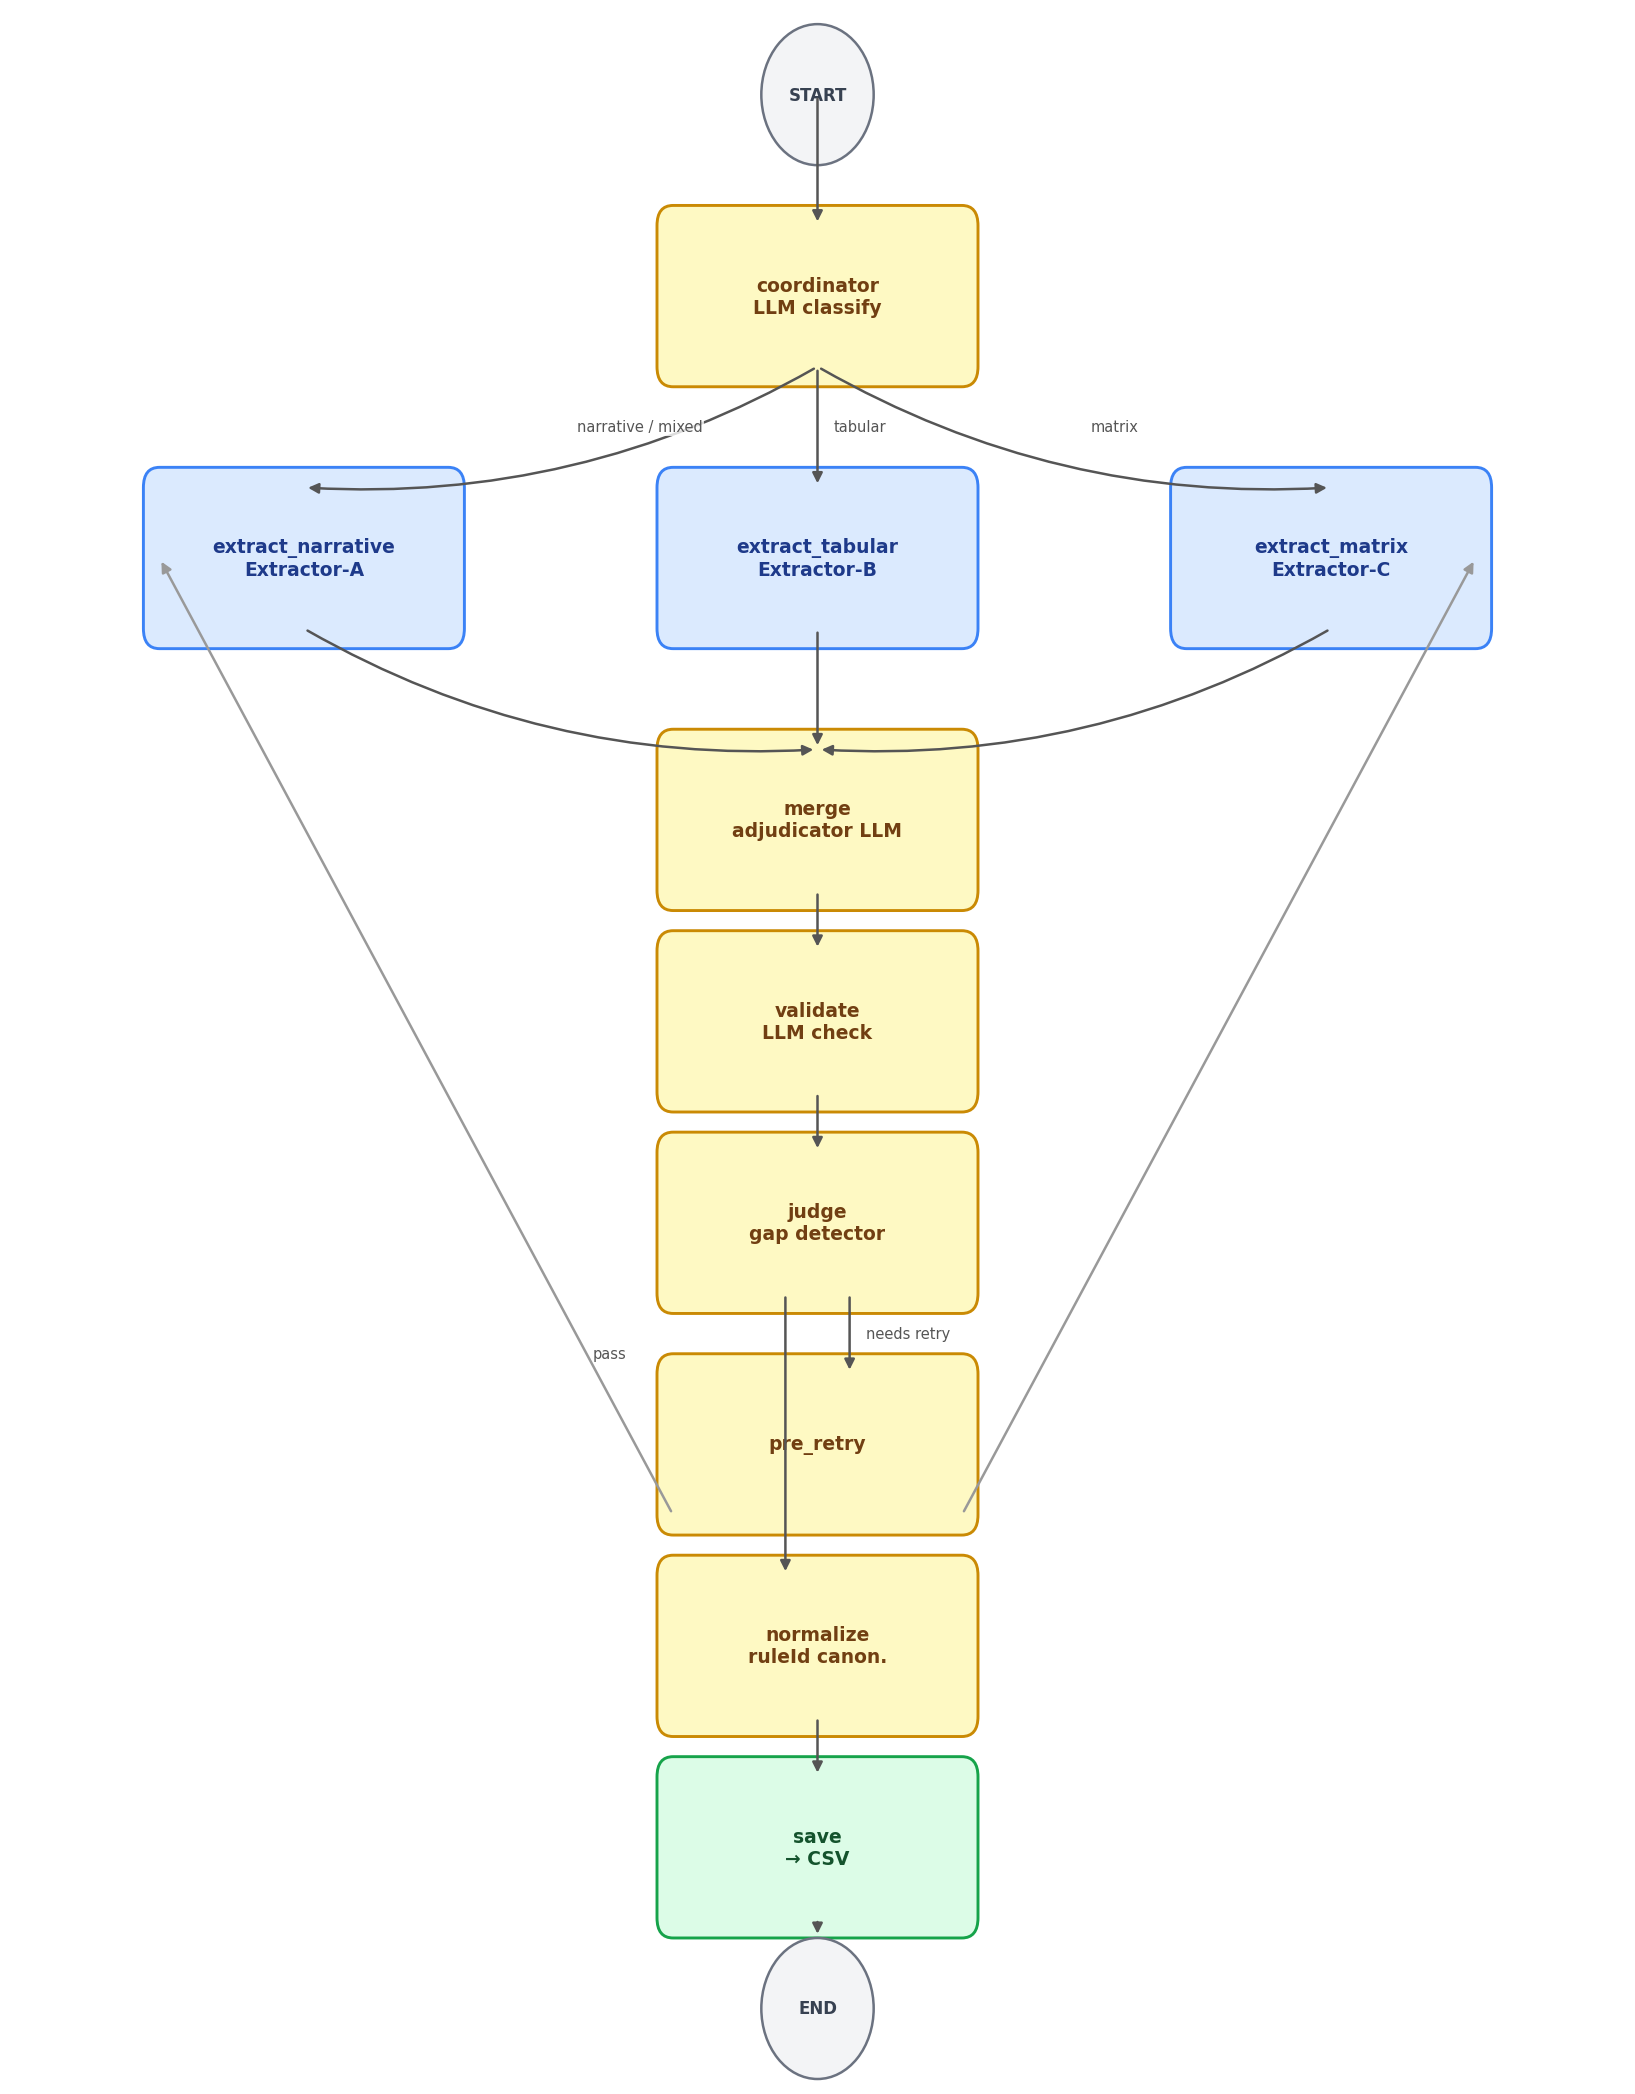
\includegraphics[width=0.86\textwidth]{layers/layer_2/pipeline_full.png}
\caption{The LangGraph pipeline. Blue nodes are LLM agent roles, yellow nodes are
deterministic, green is output. Starred stages in the text correspond to the
three-wide rows here: \texttt{scout} and \texttt{audit} are instantiated once per
document chunk and dispatched concurrently, so the three boxes denote ``one of
these per chunk'' rather than exactly three. The grey edge on the left is the
conditional bypass taken when no chunk produced records to audit. The figure is
generated from the pipeline module's own constants, so the model names, the chunk
size and the concurrency limit shown cannot drift from the code that runs.}
\label{fig:pipeline}
\end{figure}

Three properties of the topology are worth reading off the figure before the
stages are described individually, because each is a design decision rather than
an implementation detail.

\textbf{Two of the six stages use no language model at all.} Segmentation and
assembly are deterministic code (yellow). This matters for what can be claimed
about the output: the boundaries at which text is cut, the line numbers records
cite, the grouping of facts into rows, and the renaming of fields to their
canonical form are all reproducible operations that do not vary between runs. The
non-determinism discussed in Section~\ref{sec:determinism} enters only at the
three blue stages.

\textbf{The two fan-out stages are per chunk; the inducer is per corpus.} Scout
and audit scale with document length, so their cost is linear in the corpus and
they run at a bounded concurrency. The inducer runs exactly once no matter how
large the corpus is, because its input is not the corpus but the inventory of
field names the scouts reported. The narrow waist in the middle of the figure is
therefore not a drawing convention: it is the one point where the pipeline takes
a corpus-wide view.

\textbf{The \texttt{scout} $\rightarrow$ \texttt{induce} edge is a fan-in, not a
pass-through.} Every scout branch must return before the inducer runs, since an
arbiter shown one chunk's vocabulary could not reconcile it with another's. This
is the only synchronisation barrier in the graph, and it is why the inducer
cannot be merged into the scout stage however tempting the saving in calls.

\subsection{Stage 1: Segmentation and Line Numbering}
\label{sec:stage_segment}
Segmentation uses no LLM. Each document is split on blank lines into blocks,
blocks are packed into chunks of approximately 3\,500 characters, and, most
consequentially, every content line is assigned a number by code.

Numbering lines in the harness rather than asking the model to track provenance
is what makes grounding checkable later. An agent is only ever asked to cite a
line number it is currently looking at, which is among the most reliable things a
language model can be asked to produce; the alternative, asking a model to
reproduce the text it drew from, invites paraphrase and cannot be verified
automatically.

Section headings are detected by shape alone (a short, isolated, unpunctuated
line) and carried into every chunk they cover. Without this, the answer to
``which asset does this table belong to'' is lost at the first chunk boundary,
because the heading naming the asset sits in the preceding chunk. Detection by
shape rather than by a pattern of known heading formats is again a consequence of
the no-schema constraint.

\subsection{Stage 2: Scout Agents}
\label{sec:stage_scout}
One LLM call per chunk, issued in parallel with a concurrency of four. The scout
reads a numbered chunk and emits one record per rule \emph{the document itself
delimits}: a printed rule identifier where the document prints one, otherwise
one table row, one matrix cell, or one rule-stating sentence.

Two properties of the scout prompt carry the schema-agnosticism:

\begin{itemize}
    \item \textbf{Field names are copied from the document's own labels.} A
          table's column headers become the record's field names; a matrix's axis
          labels become its subject and field name; a sentence contributes the
          quantity it names. The scout is never given a set of fields to fill, so
          it cannot force a document into a foreign shape, and a corpus whose
          rules genuinely carry fourteen distinct slots yields fourteen fields
          because fourteen were observed.
    \item \textbf{No worked example is supplied.} An example demonstrates one
          particular document shape, and a model shown one reproduces that shape
          on documents that do not have it. This is the mechanism by which a
          schema-specified prompt achieves high accuracy on the corpus it was
          written for and transfers poorly; omitting the example gives up the
          former to avoid the latter.
\end{itemize}

The prompt ends with a chain-of-thought instruction: reason through the chunk,
then emit JSON. This is the \texttt{cot\_basic} paradigm, and its selection from
the grid of Section~\ref{sec:grid_search} is constrained before it is empirical.
Only three grid paradigms outscore it, and two of them cannot be carried into a
schema-agnostic scout at all: \texttt{reflexion\_guided}'s final turn is a
corpus-specific checklist, and \texttt{reflexion} inherits mandatory
sensor-naming constraints from its \texttt{graph\_informed} base, so in both
cases the margin is bought with exactly the corpus knowledge this pipeline is
defined not to have. The third, \texttt{pre\_act}, does transfer and is
statistically tied with \texttt{cot\_basic} ($0.894 \pm 0.009$ against
$0.892 \pm 0.005$); \texttt{cot\_basic} is preferred for its lower run-to-run
variance, and because \texttt{pre\_act}'s preliminary survey of document
structure has little to survey on the single chunk a scout reads.

\subsection{Stage 3: Schema Induction}
\label{sec:stage_induce}
One LLM call per corpus, and the only stage with a global view. The inducer never
sees a document. Its input is the inventory of field names and category labels
the scouts actually produced, with occurrence counts and sample values, and its
task is to merge synonyms into one corpus-level schema.

Deriving the schema from what the corpus was observed to contain, rather than
proposing one in advance from a document's opening pages, is what allows the
field count to follow the evidence. It also resolves the problem that two
documents in one corpus may name the same role differently: reconciliation
happens here, once, so that the pipeline's output is expressed in a single
vocabulary even though its scouts spoke several.

Whether that reconciliation improves agreement with a given ground truth is a
separate question from whether it is desirable, and the two can diverge: an
annotator's field names are the scoring target, so renaming a field to a
canonical form that differs from the annotator's reduces measured agreement even
where the canonical form is the better output. This stage is therefore included
on output-quality grounds, and no claim is made here about its effect on
$F1_{\text{content}}$.

What can be measured without a field-name ground truth is whether the induction
behaves as a stable function of the corpus or as a fresh invention on every run,
and the five production repeats answer this, because each run saved its induced
schema. Stability tracks how much discretion the documents leave the scouts. The
development corpus is the most stable of the four: $34$--$44$ canonical fields
per run, a mean pairwise Jaccard overlap of $0.813$ between the runs' field
sets, a core of $31$ of $50$ union fields present in every run, and the same
choice of all three role pointers on every repeat. The three external corpora
leave the scouts more discretion and the induced vocabulary varies
correspondingly (mean pairwise Jaccard $0.447$--$0.476$), around a smaller core
($9$ of $47$ union fields on desalination, $15$ of $71$ on biogas, $19$ of $86$
on sulfuric acid), and on those corpora the role pointers are not always chosen
identically across repeats. The variation originates upstream rather than in the
arbiter: the inducer sees only the inventory that run's scouts reported, so what
varies is what was observed, not what was reconciled. This inherited vocabulary
variation is also precisely what a field-name-sensitive score would convert into
noise; the content-first metric's indifference to field names is what keeps the
reported spread at $\pm 0.043$ or below despite a canonical vocabulary that
overlaps run-to-run by less than one half on three corpora.

Withholding the documents from this stage is deliberate. An arbiter that could
read the source text would be able to introduce fields no scout reported, which
would make the schema a product of the arbiter's priors rather than of the
corpus. Restricting it to the observed inventory means the schema cannot contain
anything the corpus did not exhibit.

\paragraph{What this stage's cost scales with.}
Because the inducer reads the inventory rather than the corpus, its input is
bounded by the number of \emph{distinct} field names and category labels the
scouts reported, not by the number of documents or their length. On the
development corpus, four documents totalling about $13{,}500$ characters yield
$449$ extracted facts but only $36$--$51$ distinct field names and $11$ distinct
category labels across the five runs, which with counts and sample values is a
prompt of a few hundred tokens. Every other stage is per-chunk and parallel, so
this single global call is the only place where a corpus-wide quantity enters
one context window.

That bound is a property of the architecture; whether it stays small on a
facility-scale corpus is not established by four documents, and the growth
observed here does not yet flatten. Accumulating the distinct field names
document by document on the development corpus gives $9$, $22$, $28$, $41$ in
one representative run: still rising at the fourth document. The inventory
therefore grows with vocabulary diversity, and the point at which vocabulary
diversity saturates for a real facility is unmeasured. What can be said is that
the quantity at risk is the inventory rather than the text, that it is one to
two orders of magnitude smaller than the corpus at this scale, and that its
format (a bag of names with counts) admits hierarchical merging of per-document
inventories should it ever exceed a context window. No such merging is
implemented or tested here, and the scale limitation is restated in
Section~\ref{sec:lim_scale}.

One implementation detail must be declared alongside that argument, because it
would bind before the context window does. The inventory handed to the arbiter
is truncated to the $120$ most frequent field names. On the corpora evaluated
here the cap never engages --- the largest inventory any single run produced is
$44$ names --- so no reported figure is affected by it. But the truncation is
by frequency, which means the first names discarded at scale would be the rarest
ones, and those are precisely the names the arbiter's own instructions tell it to
preserve: a field used by three records out of two hundred is the only place
those three records' information lives. Past roughly $120$ distinct field names
the implementation would therefore contradict its own specification, silently and
without error, discarding rare vocabulary before the arbiter is ever consulted.
This is a property of the current implementation rather than of the design ---
the cap exists to bound one prompt's size and could be replaced by the
hierarchical merge described above --- but it is the concrete point at which
this stage stops scaling, and it is nearer than the context window.

No claim of scalability is made anywhere in this thesis, and this is the reason.
The pipeline is demonstrated on nine documents across four corpora; what happens
at a facility holding thousands of procedures is untested, and the paragraph
above identifies the specific mechanism that would fail first and the specific
class of information it would discard --- the rarest fields, which in a safety
setting are frequently the ones carrying edge-case triggers. Naming that
mechanism is not the same as having solved it.

\paragraph{The shape a scalable version would take.} The route out is described
here because a limitation is more useful when the reader can see what would
remove it, and it is described as a sketch because none of it is implemented or
evaluated in this thesis. The single global call would become a reduction over
a tree. Each document's scouts emit a local inventory; inventories are merged
pairwise, each merge reconciling exactly two vocabularies and emitting canonical
names together with the aliases that were folded into them; the merged result is
itself an inventory, so the operation composes, and the root sees a bounded
number of canonical names rather than the union of every raw one. The number of
rounds is logarithmic in the document count, and the input to any single call is
bounded by the width of one merge rather than by the size of the corpus, which
is the property the current implementation lacks.

Two things would have to hold for that to be an improvement rather than a
rearrangement. Retaining the alias list at every level is what keeps the mapping
from a document's own label to the canonical name recoverable, without which the
provenance guarantee of Section~\ref{sec:stage_segment} would not survive the
merge. And rarity would have to stop being the discard criterion: a name should
be removed only when a merge finds it synonymous with a name that is kept, never
because it was infrequent, which is the precise inversion of what the $120$-name
truncation does today. Whether pairwise merging preserves vocabulary as well as
one global view does is an empirical question this thesis does not answer.

\subsection{Stage 4: Deterministic Assembly}
\label{sec:stage_assemble}
No LLM. Records are grouped by the document's own record boundary, each field is
renamed to its canonical name from the induced schema, and one row per rule is
emitted. The boundary is defined concretely. Where the document prints an
identifier for a rule (a rule code such as \texttt{OP-ST-001}, a coded table
row), that identifier is the boundary: two scouted readings carrying the same
printed identifier merge into one record, which is what reunites a rule restated
on both sides of a chunk boundary. Where no identifier is printed, the boundary
is the physical source line together with the order the record was read in, and
id-less records are never merged, because one line may legitimately state
several distinct rules (a matrix line holds one per cell) and a redundant record
is recoverable downstream whereas a silently merged one is not. Granularity is
thus decided by evidence printed in the document rather than by any convention
the pipeline carries.

This is the stage that gives rise to the granularity mismatch analysed in
Section~\ref{sec:granularity}. Extraction proceeds at the finest granularity the
document supports (one atomic fact per cell or value) because that choice
loses no information, whereas a coarser choice cannot be undone. Whether a given
ground truth annotates at that same granularity is outside the pipeline's
knowledge, and the metric charges the difference as error.

\subsection{Stage 5: Grounding Audit}
\label{sec:stage_audit}
One LLM call per chunk, again in parallel. The auditor re-reads each assembled
record against the numbered lines that record cites, and drops or corrects
anything not actually stated there. This stage targets numeric
hallucination: a threshold the model invented is not present on the line it
claims to come from, and the citation created in Stage~1 is what makes that
discrepancy checkable in principle.

One safeguard applies. A whole-chunk rejection (an auditor claiming that every
record from a chunk is ungrounded) is treated as an audit failure rather than
as a finding whenever the chunk carried three or more records, and the records
are retained. The reasoning is a declared design assumption rather than a
measured frequency: a verdict rejecting every record in a sizeable chunk is more
plausibly a failure of the audit call itself --- a malformed or truncated reply,
or a verdict list that did not follow the requested form --- than a correct
judgement that a whole section of an operating document states nothing.
Without the guard, one bad audit response silently deletes a document's entire
contribution. For a chunk carrying only one or two
records the guard does not apply and the rejection stands, because at that size
rejecting everything is indistinguishable from the auditor doing its job on a
record or two, and no inference of malfunction is available.

The foregoing states the stage's purpose and mechanism. It is not a claim that
the stage raises $F1_{\text{content}}$: what the audit targets is whether a
record asserts something its cited line does not support, and
Section~\ref{sec:lim_metric_blind} establishes that the metric used here checks
that property only weakly. How often the stage intervenes is therefore measured
directly instead. The pipeline writes every auditor verdict to a per-run
sidecar file, so the rate is read off the reported batch itself rather than
inferred: across the 20 runs behind Table~\ref{tab:main_results}, 1176 records
were audited in 80 chunk audits, \emph{none} was dropped, and 12 were
corrected --- an intervention rate of $1.02\%$. No chunk-level rejection
override was triggered on any run. The rate is not uniform across corpora: it is
$0.15\%$ on the development corpus and $0\%$ on desalination, against $5.71\%$
on biogas and $1.22\%$ on sulfuric acid, so what the stage does depends on the
document rather than being a constant property of the configuration. The
aggregation is produced by a script over the retained sidecars and is in the
accompanying repository.

Three conclusions follow. The first bounds the stage's effect on the reported
figures, the second says what the stage nonetheless does, and the third
restrains what may be inferred from either.

First, the arithmetic isolates which stages drive the reported performance, and
it does so without an ablation run. A record's contribution to
$F1_{\text{content}}$ can be altered by the audit only if the audit drops that
record or changes any part of its content. Zero were dropped and $12$ of $1176$
were corrected, so at most $1.02\%$ of records differ from what assembly
produced. Inspecting those twelve is informative in itself: eight rewrote the
field \texttt{lines}, which holds a record's own provenance rather than any rule
content, and only four altered a field carrying extracted content. The eight are
not excluded from the bound --- the defect described below puts that provenance
into the scored blob, so they could in principle move a score --- but rescoring
with the field removed shows they do not, which leaves the auditor's substantive
intervention across the entire reported batch at four records in $1176$.

What these figures establish is attribution. The extraction performance reported
in Table~\ref{tab:main_results} is produced almost entirely by the scout and
assembly stages, with the audit contributing negligibly to $F1_{\text{content}}$
on these corpora; the headline numbers therefore stand on the scouts' and
assembly's output essentially unedited. The same bound disposes of the converse
worry --- that the precision in Table~\ref{tab:main_results} might be an
artifact of aggressive silent filtering --- since an auditor that removes
nothing filters nothing.

Second, the stage is not inert, and the per-corpus rates are what show it. An
intervention rate of $0\%$ on desalination against $5.71\%$ on biogas is not
noise around a constant; it is the stage responding to different documents
differently, which is the behaviour a conditional safeguard should exhibit. What
it never did, on any corpus, was drop a record.

The eight provenance rewrites noted above are a defect rather than a behaviour,
and are declared here because the audit log in the accompanying repository shows
them plainly. The pipeline maintains a set of internal keys --- a record's
identifier, its category, its cited lines, its source file --- which are
bookkeeping rather than extracted content, and the scout stage filters them out
of the fields it reports. The auditor's correction path does not apply the same
filter, so a verdict returning a correction keyed \texttt{lines} writes that
record's own line numbers into its content, where they become a column of the
output and enter the scored blob. Because the metric extracts numbers from that
blob, the concern is specific: injected line numbers are numbers, and the
numeric term carries $40\%$ of the agreement score. The effect was therefore
measured rather than presumed. It reaches eight records of one corpus across the
twenty reported runs --- three each on two biogas runs and two on a third ---
and rescoring those runs with the field excluded returns $0.725 \pm 0.012$
against the reported $0.715 \pm 0.023$. The defect therefore costs the biogas
figure $0.011$, carried entirely by the two runs where the injected field is
populated, each of which loses $0.027$.

That cost is itself a consequence of the numeric term being symmetric
(Equation~\ref{eq:numoverlap}), and the comparison is worth stating because it
is the clearest demonstration of what the second direction buys. Under the
recall-only alternative the same defect costs \emph{exactly nothing}: the
injected line numbers are surplus values, a recall-only term prices surplus
values at zero, and the corpus scores $0.725 \pm 0.012$ whether the field is
present or not. A metric that cannot see a record asserting numbers its source
line never contained is not one that should be trusted to detect a hallucinated
threshold either, and this defect --- introduced by accident --- is the closest
thing to a controlled injection test these corpora provide.

The direction of the bias should be stated plainly: the reported biogas figure
is \emph{depressed} by $0.011$ relative to what the pipeline would score without
the defect, so it is conservative rather than flattering. The repair is one line
--- the correction path must apply the same internal-key filter the scout path
already applies --- and it is not applied here because doing so changes
extraction output, which requires re-running every corpus, and a fresh batch
differs from this one by the endpoint's own run-to-run variation: up to $0.049$
on the corpora reported here. Re-running would move every figure in this thesis
by more than the defect it removes, and in an unknown direction, so the defect is
disclosed and bounded instead, and carried in the code with a comment recording
all of the above. It should be fixed together with the next full re-run, when the
cost of re-measurement is being paid for other reasons anyway.

Third, and restraining both of the above, a drop count of exactly zero across
$1176$ audited records is consistent with two different
explanations, and the measurement alone does not separate them: either there was
almost nothing to find, or an auditor served by the same model as the scout
cannot see what the scout got wrong. The two are not equally supported here. The
field-level verification of Section~\ref{sec:field_verification} is an
independent check on the same records, performed against the source documents by
deterministic code rather than by a model, and on the three runs where a
correspondence can be established it finds every bound cell carrying the printed
value in the printed column; the only cells where the pipeline and the
annotation disagree are four where the annotation is wrong. On those runs there
was in fact little for the auditor to catch, which is what its
intervention rate of $0.15\%$ would predict. That argument reaches one corpus and
one failure mode. It does not show that a shared-model auditor would catch
hallucinations produced by a scout that had, for whatever reason, misread a
noisier document: a checker drawn from the same weights as the writer is a
correlated check, and correlated checks fail together. Role independence is
available as a command-line override
(Section~\ref{sec:model_assignment}); measuring whether it raises the
intervention rate would require a second model of comparable strength, which
this study does not have, and injecting hallucinations deliberately to see
whether the stage catches them is an experiment these corpora do not pose.

\subsection{Model Assignment}
\label{sec:model_assignment}
All three agent roles are served by \texttt{gemma4:31b}, for the reason given in
Section~\ref{sec:experimental_conditions}: over 100 grid runs it outperformed the
alternative on all ten paradigms, by a margin comparable to the spread between
paradigms, and there is no measured basis for assigning any role to the weaker
model. Role independence between scout and auditor is available through a
command-line override; it is not the default because the only alternative
measured here was both weaker and less stable, and an unreliable auditor removes
more correct records than incorrect ones.

\subsection{Error Resilience}
\label{sec:resilience}
Three failure modes are handled explicitly, each because it was observed to occur
against a hosted endpoint rather than anticipated in the abstract.

\textbf{Empty content from a reasoning model.} A model that returns its
deliberation in a separate field and its answer in the content field can exhaust
the output budget before the answer begins, yielding an empty content string with
a length-based finish reason. Parsing that as an empty result would silently
record ``this chunk contained no rules''. It is instead raised and retried.

\textbf{Truncation.} A reply cut off at the output budget loses every record
after the cut. This is detected from the finish reason and surfaced as a warning
rather than absorbed, since the symptom otherwise appears as an unexplained drop
in record count.

\textbf{Transient endpoint failures.} Calls are attempted up to three times with
exponential backoff from a 15\,s base. The timeout is deliberately generous at
600\,s: reasoning models with a large output budget legitimately take minutes,
and a shorter timeout discards valid work in progress.


\section{Results}
\label{sec:results}

Every figure in this section is a mean over five repeats of the same
configuration, reported with its standard deviation, for the reason given in
Section~\ref{sec:determinism}: a single run against a hosted endpoint is one
draw, and two configurations whose intervals overlap are tied rather than ranked.
Precision is reported alongside the ceiling that Equation~\ref{eq:ceiling}
imposes on it, since the two are not comparable across corpora without it.

\subsection{Extraction Across Four Corpora}
\label{sec:results_main}

Table~\ref{tab:main_results} reports the pipeline on the development corpus and
on the three external corpora, none of which contributed to any configuration
choice. No prompt, parameter, field mapping, or threshold was changed between the
four; the pipeline was invoked identically in each case, differing only in the
input directory. The corpora do differ in how much of the pipeline's development
they were visible for, which Section~\ref{sec:lim_exposure} sets out.

\begin{table}[H]
\centering
\caption{Multi-agent pipeline, five repeats per corpus. Rows are ordered as in
Table~\ref{tab:corpora}: the development corpus first, then the three external
corpora in the order they were introduced. The ordering is deliberately
independent of the scores, so that the table cannot be read as leading with its
best result. \emph{Max~P} is the ceiling that the record count imposes on
precision (Equation~\ref{eq:ceiling}); precision must be read against it rather
than against $1.0$.}
\label{tab:main_results}
\small
\begin{tabular}{llrrrrrr}
\toprule
\textbf{Corpus} & \textbf{Role} & \textbf{GT} & \textbf{Records} &
\textbf{$F1_{\text{content}}$} & \textbf{P} & \textbf{Max~P} & \textbf{R} \\
\midrule
Production line (iMAKS)  & dev      & 86 & $131.0 \pm 0.0$ & $0.719 \pm 0.000$ & 0.595 & 0.656 & 0.907 \\
\midrule
Biogas digestion         & external & 47 & $28.0 \pm 0.0$ & $0.715 \pm 0.023$ & 0.957 & 1.000 & 0.570 \\
RO desalination          & external & 26 & $27.2 \pm 0.4$ & $0.850 \pm 0.019$ & 0.831 & 0.956 & 0.869 \\
Sulfuric acid            & external & 70 & $49.0 \pm 1.0$ & $0.649 \pm 0.049$ & 0.788 & 1.000 & 0.552 \\
\bottomrule
\end{tabular}
\end{table}

Four observations follow. The first fixes the reference point, the second is the
central result, and the last two constrain how the table should be read.

\textbf{The development corpus, where the pipeline was built, scores
$0.719 \pm 0.000$.} This is the figure every other number in the table should be
compared against, because it is the only corpus whose documents were available
while the pipeline was being written. It is reported first for that reason rather
than because of where it falls in the ranking. Its recall of $0.907$ is the
highest of the four and its precision of $0.595$ the lowest, a pattern the second
and third observations explain.

\textbf{Performance does not fall away on unseen material, but neither is it
uniform.} The three external corpora score $0.715$, $0.850$ and $0.649$ against
the development corpus's $0.719$. One sits above it, one essentially level with
it, and the third, sulfuric acid, sits $0.070$ below. The honest reading is
therefore not that unseen corpora are handled as well as the development corpus
in every case, but that the development corpus holds no privileged position: it
is neither the best nor the worst of the four, which is the pattern a system
shaped around its evaluation data would not produce. The spread across the four
corpora, $0.649$ to $0.850$,
is wider than any single corpus's run-to-run variation, so the differences
between corpora are real and demand explanation rather than averaging. The two
observations that follow supply it, and in both cases the explanation is
annotation granularity rather than extraction error.

\textbf{The development corpus is precision-limited by granularity, not by
error, and one observation demonstrates this outright.} Across the five dev
repeats both the number of true positives and the number of records emitted are
\emph{identical}: 78 of 86 ground-truth rows matched from 131 records, every
run, giving $F1 = 0.719$ with zero variance. The 131 records against 86
annotated rows put a ceiling of $0.656$ on precision before a single comparison
is made, and the observed $0.595$ must be read against that ceiling rather than
against $1.0$. The same rules were found each time and only their itemisation
differs from the annotation's; $F1_{\text{content}}$ charges that difference as
error. The unpaired records state facts the source documents contain and the
annotation schema has no row for, such as the inter-station dependencies printed
in a table the ground truth does not cover; every value they assert appears in
the document they cite, which Section~\ref{sec:lim_gt} measures rather than
assumes.

\textbf{Variance differs sharply across corpora, and a zero standard deviation
does not mean determinism.} Sulfuric acid's standard deviation of $0.049$
(range $0.610$--$0.733$) is the largest of the four; biogas's is $0.023$
and desalination's $0.019$. The development corpus returned an identical $0.719$ on
all five repeats, and biogas an identical record count on all five. Neither is
evidence of a deterministic pipeline. The five runs behind each figure are
genuinely independent calls --- the response cache is disabled automatically
whenever repeats are requested, precisely so that a warm cache cannot replay one
run five times and report the result as zero variance --- and the underlying
prediction files differ from one another in every case. What converges is the
score, not the output: on the development corpus all five runs recovered the
same 78 ground-truth rows from the same number of records, so the differences
between them fell entirely in field naming and category labelling, which
$F1_{\text{content}}$ is designed not to charge for. A corpus can therefore
report a zero standard deviation and still be varying underneath, and a batch of
five repeats should not be read as capturing the full spread of a hosted
endpoint that is non-deterministic for long generations. This is why two
configurations whose intervals overlap are treated as tied throughout this
thesis.

\subsection{Field-Level Verification Against the Source Documents}
\label{sec:field_verification}

$F1_{\text{content}}$ deliberately ignores field identity
(Section~\ref{sec:no_field_matching}), so it cannot answer the question a
downstream consumer actually needs answered: is each value in the right slot? A
knowledge graph populated from these records needs the critical low bound to be
the critical low bound, not merely a number that appears somewhere in the row.
This section answers that question directly, outside the metric, by comparing
cells against the ground truth on the one corpus where a field correspondence can
be established without inventing one.

The correspondence is obtained by normalising both sides' column names (case
folding and separator removal) which maps the ground truth's \texttt{critLo},
\texttt{warnLo}, \texttt{warnHi}, \texttt{critHi} onto the pipeline's
\texttt{crit\_lo}, \texttt{warn\_lo}, \texttt{warn\_hi}, \texttt{crit\_hi}. No
vocabulary is consulted; the match is a string operation. Records are keyed by
station and sensor, which makes the check conditional on the extraction having
attached a station to its threshold records --- and that turns out to be the
finding rather than a precondition.

\textbf{Result: the check succeeds completely on three of five runs and not at
all on the other two.} On runs three, four and five all $22$ of the ground
truth's threshold sensors are recovered and $84$ of $88$ bound cells sit in the
field the annotation assigns them to, the same $84$ in each run. On runs one and
two the threshold records carry no station value, no record can be keyed against
the annotation, and the check recovers nothing: $0$ of $22$ sensors. Pooled over
all five runs the figure is therefore $252/440$ bound cells, or $57.3\%$, and
that pooled number describes a bimodal outcome rather than an average one.

This is the sharpest available demonstration of what
Section~\ref{sec:lim_metric_blind} claims in the abstract. The five runs differ
enough that field-level correspondence is impossible to establish on two of
them, and $F1_{\text{content}}$ reports $0.719$ on all five, identically, with a
standard deviation of zero. A difference that destroys slot-level checkability
on $40\%$ of runs is completely invisible to the headline metric, because the
values are still present in the record and the metric reads a bag of values. Any
deployment that needs slot-level guarantees must therefore verify them
separately, as this section does, and must expect that verification to fail on
runs the headline number cannot distinguish.

The four cells that do mismatch on the three keyable runs are worth examining,
because they are not extraction errors.

\textbf{The residual disagreements are ground-truth errors.} The source table for
\texttt{ST03\_LABELLING} reads, under the printed header
\texttt{Sensor | Unit | CRIT\_LO | WARN\_LO | Nominal | WARN\_HI | CRIT\_HI}:

\begin{lstlisting}
| SPD | m/s | 0.65 | 0.75 | 0.85 +/- 0.01 | 0.95 | 1.05 | ...
\end{lstlisting}

The pipeline extracts $\texttt{crit\_lo}=0.65$, $\texttt{warn\_lo}=0.75$,
$\texttt{warn\_hi}=0.95$, $\texttt{crit\_hi}=1.05$, the document's values, in
the document's columns. The ground truth records $1.05$, $1.15$, $1.35$ and
$1.05$ for the same four fields. Those numbers appear nowhere in the source, and
the annotation assigns \texttt{critLo} and \texttt{critHi} the same value
($1.05$), which is not a well-formed threshold range. The same pattern holds for
\texttt{ST04\_PACKAGING}, where the source states $\texttt{CRIT\_LO}=0.85$ and the
annotation records $1.25$. Scored against the source documents rather than the
annotation, field placement on the three keyable runs is $88/88$ in each ---
every bound cell the extraction produced carries the value the source document
prints, in the column the source document prints it in.

Two conclusions follow, and both bear on how the headline figures should be read.
First, where the correspondence can be established at all, the extraction places
values correctly at a rate the row-level metric cannot express: a corpus-level
$F1_{\text{content}}$ of $0.719$ coexists with exact field placement against the
source documents on the rules that carry numeric bounds. The two measure
different things, and the lower number is not evidence of misplaced values ---
though neither, as the bimodal result above shows, is the higher one evidence
that placement is reliable run to run. Second, the ground truth against which every figure in this thesis is
computed contains errors of its own: four specific cells, in a document any
reader can open. Reported precision is therefore a lower bound on correctness
rather than a measurement of it (Section~\ref{sec:lim_gt}).

\textbf{One practical caveat for any consumer of these records.} The column
holding the station identifier is not stable across runs: in one run it is
\texttt{station}, in the others the value sits in \texttt{asset} while an empty
\texttt{station} column also exists. Resolution must therefore take the first
non-empty value among candidate columns \emph{per row}, not choose one column per
file. This is the naming drift discussed in Section~\ref{sec:stage_induce},
appearing exactly where the source document does not print an explicit header for
the concept.

\subsubsection{A Weaker Binding Check That Does Reach the External Corpora}
\label{sec:binding_check}
The verification above requires a column-name correspondence and therefore stops
at the development corpus. A weaker form of the same question can be asked of
every corpus without constructing any correspondence, using only two things
neither side must be told: which of the ground truth's \emph{own} columns holds
each role (its low bound is whatever its low-bound column contains), and the
internal structure of the predicted record. For every pair the assignment
accepted, each populated ground-truth role value is located inside the paired
record: in exactly one scalar field, inside a free-text field, in several
fields, or nowhere. If the extractor binds values to slots, the same discovered
field should receive a given role in every pair, corpus-wide.

It does. On biogas, the ground truth's low bound lands in the record field the
document calls \texttt{ll} in $26$ of $26$ slot-bound cases and the high bound
in \texttt{hl} in $10$ of $10$; on desalination the min and max bounds land in
one consistent field in $20$ of $20$ cases each; on the development corpus the
modal consistency per threshold role is $0.95$--$1.00$. The sulfuric acid
annotation poses no slot-binding question at all: it records every quantity in a
single \texttt{numeric\_value} column, so there are no distinct numeric roles
that could be swapped, and the check degenerates. What can be asked there is the
weaker record-level question, and the ground-truth value appears within the text
of the \emph{matched} record in $121$ of $136$ checks. Across the three external
corpora, $89$--$100\%$ of ground-truth role values are present in the record the
metric paired them with.
The check is deliberately weaker than the development-corpus verification, and
the weakness has a precise form worth naming: consistency is not correctness. An
extractor that placed every low bound in the high slot would do so consistently,
and would score a perfect modal share on this test. Consistency establishes that
values are bound to slots rather than scattered; it does not establish that the
slot is the right one.

That stronger question can be asked wherever the two vocabularies happen to
coincide without being made to, which they do on two corpora: the development
corpus (\texttt{critLo}, \texttt{warnLo}, \texttt{warnHi}, \texttt{critHi} against
the pipeline's \texttt{crit\_lo}, \texttt{warn\_lo}, \texttt{warn\_hi},
\texttt{crit\_hi}) and desalination (\texttt{min\_bound}, \texttt{max\_bound}).
For every accepted pair, each ground-truth numeric value is first sought
anywhere in the paired record, and only then asked whether it sits under the
matching name. The two questions are kept apart deliberately, because a value
the extraction never produced is a recall miss and a value it produced but filed
elsewhere is a binding error, and adding them together would report the first as
the second.

On the development corpus $600$ of $920$ ground-truth numeric cells are present
somewhere in their paired record, and of those $420$ --- $0.70$ --- sit in the
correspondingly named slot. On desalination all $50$ are present and $40$ ---
$0.80$ --- are correctly placed. These are the only direct measurements of slot
correctness this thesis can make, and they should be read as the honest ceiling
on what the extraction offers a downstream consumer: roughly three quarters of
the values it recovers are where a consumer would look for them, and the
remaining quarter are somewhere else in the record. That figure is invisible to
$F1_{\text{content}}$ by construction, which is why it is measured here rather
than inferred from a headline score.

\subsection{The Cost of Requiring No Schema}
\label{sec:results_grid}

The grid of Section~\ref{sec:grid_search} supplies the prompt with the
development corpus's schema, rule taxonomy, identifier convention, and worked
examples drawn from that same benchmark family. Table~\ref{tab:grid_contrast}
reports the leading grid conditions rescored with the metric of
Section~\ref{sec:metrics}, so that both sides of the comparison are produced by
the same evaluator on the same ground truth. A figure produced by a different
metric could not be placed beside these.

\begin{table}[H]
\centering
\caption{All three approaches on the development corpus, five repeats each,
scored by $F1_{\text{content}}$. Rows are grouped by \emph{what each system was
given}, not by score, because that is the variable the table actually
manipulates. \emph{Ceiling} is the highest $F1_{\text{content}}$ each system
could reach at its own record count (Equation~\ref{eq:ceiling}) if every record
it emitted were correct; \emph{head} is the distance left to it. Only the
bottom group can be run on a corpus nobody has configured it for.}
\label{tab:grid_contrast}
\small
\begin{tabular}{llrrrrrr}
\toprule
\textbf{System} & \textbf{Given} & \textbf{Recs} & \textbf{$F1_{\text{content}}$} &
\textbf{P} & \textbf{R} & \textbf{Ceil.} & \textbf{Head} \\
\midrule
\multicolumn{8}{l}{\emph{Per-corpus configuration supplied by a human}} \\
\texttt{gemma4:31b}, reflexion\_guided & schema & 78.8 & $0.949 \pm 0.020$ & 0.993 & 0.909 & 0.956 & 0.007 \\
\texttt{gemma4:31b}, reflexion         & schema & 77.2 & $0.939 \pm 0.008$ & 0.993 & 0.891 & 0.946 & 0.007 \\
\texttt{gemma4:31b}, cot\_basic        & schema & 70.4 & $0.892 \pm 0.005$ & 0.992 & 0.812 & 0.900 & 0.008 \\
Hand-written regex parser              & layouts + ABox & 54.0 & $0.771$ & 1.000 & 0.628 & 0.771 & \textbf{0.000} \\
\midrule
\multicolumn{8}{l}{\emph{Nothing supplied}} \\
\textbf{Multi-agent pipeline}          & --- & 131.0 & $\mathbf{0.719 \pm 0.000}$ & 0.595 & 0.907 & 0.793 & 0.074 \\
Single schema-free prompt              & --- & 134.0 & $0.733 \pm 0.015$ & 0.601 & \textbf{0.937} & 0.782 & 0.049 \\
\bottomrule
\end{tabular}
\end{table}

On F1 alone the table ranks both schema-agnostic conditions last, behind a
single schema-specified prompt and a hand-written regex parser. The grouping is
what makes that ordering interpretable: every system above the rule was handed
something a human produced by reading these four documents, and the two below it
were not, so the column the table varies is configuration rather than capability.
The two schema-free conditions differ from each other only in orchestration, and
are separated by less than either one's distance to the configured group;
Section~\ref{sec:results_ablation} takes that comparison up directly.

Two comparisons are therefore available, and they answer different questions.
\emph{Within} the configured group the comparison is like-for-like, and the
result is that schema-specified prompting beats hand-written parsing by
$0.178$ ($0.949$ against $0.771$) --- when a human is going to encode the corpus
either way, encoding it as a prompt recovers $24$ more of the $86$ rules than
encoding it as regular expressions. \emph{Across} the rule the comparison is not
like-for-like and should not be read as one. Four observations develop what it
does and does not measure.

\textbf{Recall is equal.} The pipeline recovers $0.907$ of the ground
truth against the best schema-specified condition's $0.909$: 78 of 86 rows on
every repeat in the first case, a mean of 78.2 in the second. The two systems
find the same number of rules, and the entire F1
gap opens elsewhere. Whatever the pipeline
mainly lacks, it is not coverage of the ground truth.

\textbf{The entire gap is precision, and the precision gap is granularity.} The
grid conditions are given the shape of a row, emit $70$--$79$ rows against a
ground truth of $86$, and carry a precision ceiling of $1.0$. The pipeline
extracts one record per atomic fact, emits $131$ records on every run, and is
capped by Equation~\ref{eq:ceiling} at $0.656$
before any content is examined. The comparison is therefore between a system
given the annotator's granularity convention and one that had to infer it.

\textbf{The regex parser is not beaten on F1, and no such claim is made.} Its
$0.771$ sits above the pipeline's $0.719 \pm 0.000$, so on this corpus the
parser reports the higher F1 and that is stated plainly rather than explained
away. What separates them is what each
one is. The parser's precision is perfect for a reason that is worth stating
exactly: its author read these documents and encoded their layouts by hand, and
the parser additionally references \emph{only entities the seed knowledge graph
declares}, which it reads from that graph's node file --- four stations, their
twelve sensors, and seven zones. A parser that can emit no name outside a
declared twelve-sensor inventory cannot mis-name an entity, so its $1.000$ is a
property of what it was given rather than of what it read. This is per-corpus
configuration in its purest form, and it is given more of it than either LLM
condition: the schema-specified grid is told the shape of a rule but must still
recover the entity names from the text, and the pipeline is told neither. The
cost is the recall of $0.628$: every rule outside the encoded layouts is
invisible to it, silently and unrecoverably.

Two structural facts finish the comparison, and both matter more than the
ordering. The first is that the parser is \emph{saturated}. Because every record
it emits is correct, its $0.771$ is exactly the ceiling of
Equation~\ref{eq:ceiling} for a system emitting $54$ records against $86$ rows:
its headroom is $0.000$. It is not a system that is currently performing at
$0.771$ and might perform better; it is a system that cannot improve by any
amount without a human writing more parsing code. The pipeline, at $0.719$
against a ceiling of $0.793$ at its own record count, retains headroom that
belongs to granularity rather than to error.

The second is what ``the parser'' actually is. It is not one parser applied to
four documents but four hand-written functions, one per document, dispatched on
the filename --- \texttt{parse\_sop001} through \texttt{parse\_sop004}, some
$480$ lines for four files. A fifth document produces nothing at all until
somebody writes a fifth function. The unit of effort is therefore the document,
not the corpus and not the domain, which is the property that decides where each
approach belongs: for a fixed and small set of documents that will not change,
hand-written parsing is the correct engineering choice and this thesis does not
argue otherwise. The pipeline's case rests entirely on that condition failing. The pipeline,
given none of that, recovers $0.907$ of the ground truth --- half again as much
as the parser, on a corpus the parser's author had read and the pipeline had
not been configured for. The comparison the
parser supports is therefore not ``LLM pipeline versus simple baseline'' but a
measurement of what coverage costs when the extraction patterns must be
discovered rather than authored; and unlike the pipeline, the parser transfers
to a new corpus only by being rewritten.

\textbf{The schema-specified condition is not a transferable baseline.} Its
prompt hardcodes field names, class labels, an identifier format, and worked
examples containing real station identifiers from the development corpus.
Applying it to the biogas, desalination, or sulfuric acid corpora requires a human to
read those documents and rewrite the prompt, which is the per-domain
configuration this work exists to eliminate, and, more sharply, is an instance of
adapting the extractor to the corpus it is scored on.\footnote{The claim is
about comparability, not mechanical executability, and the distinction was
checked rather than assumed: the run registry in the accompanying repository
records an exploratory application of the unmodified grid prompts to the
desalination document. They emitted $7$--$14$ records against $26$ ground-truth
rows, expressed in the development corpus's vocabulary; the outputs were not
retained and no figure in this thesis derives from them. The unmodified
condition transfers as an under-extraction in a foreign schema, not as a
baseline.}

The summary is therefore this. Where a human has already read the documents,
that reading is worth roughly $0.23$ F1 if it is written into a prompt and
$0.05$ if it is written as regular expressions, and the prompt is the better
use of the same human effort by $0.178$. Where nobody has read them, neither
configured condition has a score at all --- the grid prompt would have to be
rewritten and the parser would have to be extended with a function per document
--- and the pipeline reports $0.649$--$0.850$. The question the table settles is
not which system is best, but what the configuration those systems require is
worth, and what it costs when it is unavailable.

\subsection{What the Orchestration Buys: A Single-Prompt Ablation}
\label{sec:results_ablation}

Neither condition in Table~\ref{tab:grid_contrast} isolates the architecture.
Both are told things about the corpus that the pipeline is not, so both measure
the value of \emph{configuration}. The question left unanswered is narrower and
more uncomfortable: does the orchestration --- segmentation with line numbering,
parallel scouts, the corpus-level inducer, deterministic assembly, the grounding
audit --- do anything that one call per document would not?

The ablation holds everything constant except the graph. The same model,
endpoint, temperature, seed, retry policy and output budget; the same JSON
contract and parser; the same evaluator, ground truths and five repeats. The
prompt is the scout's own prompt with only the passages that depend on chunking
removed: the record-boundary rules, the attribute-versus-case column test, the
field-naming discipline, the verbatim-value rule, the category request and the
explicit refusal to supply a worked example are all carried over word for word,
because rewriting them would have compared two prompts rather than two
architectures. What is removed is the pipeline: no chunking, no line numbers,
no inducer, no assembly, no auditor. One document, one call, one row per
returned object.

\begin{table}[H]
\centering
\caption{The multi-agent pipeline against a single schema-free prompt, five
repeats each, same evaluator. Both conditions are given nothing about the target
schema; they differ only in orchestration. \emph{Calls} is LLM requests per run
(the pipeline issues one scout and one audit per chunk plus one inducer; the
baseline issues one per document).}
\label{tab:ablation}
\small
\begin{tabular}{lrrrrrr}
\toprule
& \multicolumn{2}{c}{\textbf{Multi-agent}} & \multicolumn{2}{c}{\textbf{Single prompt}} & & \\
\cmidrule(lr){2-3}\cmidrule(lr){4-5}
\textbf{Corpus} & \textbf{$F1$} & \textbf{Calls} & \textbf{$F1$} & \textbf{Calls}
& \textbf{$\Delta$} & \textbf{Fields} \\
\midrule
Production line (dev) & $0.719 \pm 0.000$ & 13 & $\mathbf{0.733 \pm 0.015}$ & 4 & $+0.014$ & 34--44 / 47--55 \\
Biogas digestion      & $0.715 \pm 0.023$ &  7 & $\mathbf{0.762 \pm 0.007}$ & 1 & $+0.047$ & \\
RO desalination       & $\mathbf{0.850 \pm 0.019}$ &  7 & $0.793 \pm 0.016$ & 1 & $-0.057$ & \\
Sulfuric acid         & $\mathbf{0.649 \pm 0.049}$ &  9 & $0.607 \pm 0.014$ & 3 & $-0.042$ & \\
\midrule
\textbf{Mean}         & \textbf{0.733} & & \textbf{0.724} & & $\mathbf{-0.010}$ & \\
\bottomrule
\end{tabular}
\end{table}

\textbf{The model is capable of schema-agnostic extraction on its own.} That is
the first and most useful thing the ablation establishes. Given the same
extraction discipline and no target schema, a single call per document reaches
$F1_{\text{content}}$ indistinguishable from the full pipeline's: the two win on
two corpora each, and the mean difference of $0.010$ sits far inside the
run-to-run variation of the corpora themselves, which reaches $0.049$. Two
individual gaps do exceed both conditions' spreads and are real --- biogas
favours the single prompt by $0.047$, desalination favours the pipeline by
$0.057$ --- but they point in opposite directions, so no aggregate advantage
survives. Complex orchestration is therefore not a precondition for
schema-agnostic extraction at this scale, and the result is reported plainly
because it is the more useful finding for anyone building such a system.

\textbf{Two hypotheses about where orchestration should help were tested and not
supported.} The first is that it buys stability rather than accuracy: it does
not, since the single prompt has the \emph{lower} standard deviation on three of
the four corpora, including $0.014$ against $0.049$ on sulfuric acid. Only on
the development corpus is the pipeline the steadier, and there its zero variance
is a property of the score rather than of the output
(Section~\ref{sec:results_main}). The second is that it should win where a
corpus spans several documents, cross-document vocabulary reconciliation being
the one thing a per-document call cannot do: it does not, since the pipeline
wins on sulfuric acid, which has three documents, and loses on the development
corpus, which has four. No property of the corpora tested here predicts the
direction of the difference.

\textbf{What separates the two conditions is not in the score, because the
metric does not look there.} $F1_{\text{content}}$ evaluates \emph{what} was
extracted, never \emph{how} it was obtained, and the two conditions differ
almost entirely in the latter. Two differences are concrete and checkable.

The first is provenance. Every pipeline record cites the document and the
numbered line it was read from; every baseline record cites nothing, because
line numbering was among the stages removed. The consequence is not a matter of
degree: the grounding check of Section~\ref{sec:lim_gt} --- which establishes
that all $669$ values asserted by the surplus records appear in the documents
they cite --- cannot be run on the baseline's output at all, since there is no
citation to check against. An extraction that cannot be traced to a line cannot
be audited, and in the settings this work targets that distinction has
consequences: an operator configuring an alarm from an extracted threshold needs
to see the line of the procedure it came from, and a reviewer disputing a rule
needs somewhere to look. The second is vocabulary: the inducer reconciles the
development corpus onto $34$--$44$ canonical field names where the baseline's
unreconciled output carries $47$--$55$ for the same documents. A metric that
discards field names by construction cannot charge for that sprawl, and this one
does not.

\textbf{The trade-off, stated as measured.} The pipeline issues three to seven
times as many requests for statistically indistinguishable accuracy: $13$ calls
against $4$ on the development corpus, and $7$ against $1$ on each
single-document external corpus. What those requests buy is not a higher score
but line-level traceability and a consolidated vocabulary. A reader whose
requirement is a scored rule table and nothing else should prefer the single
prompt on this evidence. A reader who must be able to say where each extracted
value came from has no such option, because the baseline does not produce that
information at any price.

\textbf{One honest narrowing of that claim.} Provenance is delivered by the
line-numbering of Stage~1 specifically, not by the graph as a whole. A single
prompt given a line-numbered document and asked to cite lines would plausibly
recover much of it, and that intermediate condition is not tested here. What the
remaining stages contribute --- the inducer's vocabulary reconciliation, the
assembly's record-boundary discipline, the audit's grounding pass --- is
therefore separable from the provenance argument and is not individually
measured. The trade-off this subsection reports is real and its two halves are
both quantified, but attributing all of it to the multi-agent design would
credit the architecture for a property one of its stages supplies.

\textbf{What this settles.} It does not show that multi-agent extraction is
unnecessary in general; four small synthetic corpora, one model and one prompt
family cannot support that. What it settles is that the accuracy in
Table~\ref{tab:main_results} is attributable to withholding the schema and to
the extraction discipline expressed in the prompt rather than to the graph, and
that the graph's contribution lies in auditability rather than in
$F1_{\text{content}}$. Whether that contribution is worth its cost depends on
what consumes the output, which Section~\ref{sec:lim_downstream} does not
evaluate and does not claim.

\section{Limitations}
\label{sec:limitations}

The limitations below are ordered by how much they bound the claims made in
Section~\ref{sec:results}, most consequential first. Several are properties of
the evaluation rather than of the pipeline, and are stated here because a reader
cannot otherwise tell how far the reported figures reach.

\subsection{Granularity Disagreement Bounds Every Reported Figure}
\label{sec:lim_granularity}
The four corpora disagree about what constitutes one rule, and no convention
among them is privileged. Where a ground truth annotates more coarsely than the
pipeline extracts, correct records become false positives by the one-to-one
assignment (Equation~\ref{eq:ceiling}); where it annotates more finely (as the
development corpus does for threshold rules, splitting one printed table row into
up to three annotated rows) ground-truth rows go unmatched and become false
negatives instead. Both occur in the same corpus simultaneously
(Section~\ref{sec:granularity}), so the discrepancy cannot be removed by a single
merge or split rule. On the development corpus the cap is $0.656$ on every
repeat and the observed precision of $0.595$ sits just beneath it. The effect is
not a marginal one: on the sulfuric acid corpus, undoing a single annotation
convention while leaving the predictions untouched moves the reported figure by
$0.147$ (Section~\ref{sec:granularity}), which is larger than the gap between
several of the corpora in Table~\ref{tab:main_results}.

No claim is made that the pipeline's itemisation is the correct one. Splitting a
threshold row into an operational band and a critical trip, or keeping them
together, are both defensible schema designs, and which is right depends on what
the rows will be used for. The point is only that the two designs are
incompatible under a bijective assignment, and that the resulting penalty is
charged to whichever side emits more rows regardless of content.

The consequence is that $F1_{\text{content}}$ as reported here conflates two
distinct things: whether the pipeline found the right rules, and whether it
itemised them the way a particular annotator did. Recall separates them
partially (it is unaffected by surplus records) which is why the
equal recall between the pipeline and the schema-specified baseline
($0.907$ against $0.909$, Section~\ref{sec:results_grid}) is the more informative
comparison. A metric
that scored a set of atomic facts against a set of composite rows without
requiring a bijection would measure the first thing alone; constructing one is
left to future work.

\subsection{The Metric Does Not Read Word Order or Attribute Binding}
\label{sec:lim_metric_blind}
Section~\ref{sec:metric_validity} establishes what $F1_{\text{content}}$
measures, and the same study establishes what it does not. Scrambling token
order within a record, against an order-preserving control, costs $0.000$; the
comparison behaves as a bag of tokens and numbers rather than as a reading of a
sentence. Moving quantities between records (the right rule carrying the wrong
bound) costs $-0.001$ -- the optimal assignment simply re-pairs each record with
the row its new content resembles, absorbing the damage by design, and on the
development corpus the score actually \emph{rises} by $0.017$ under the
perturbation -- and permuting the category label costs $+0.007$, so
neither value-to-rule binding nor label correctness is meaningfully checked.

Two consequences follow. A record that contains the right words and numbers in a
nonsensical arrangement is scored almost as highly as a coherent one. And
category-label correctness is essentially unpriced, which is consistent with
the design argument that category exact-match is unwinnable across vocabularies,
but means the pipeline's category discovery is not evaluated by the headline
figure at all. What the metric leaves unchecked about binding is examined by
separate means: directly against the ground truth's fields on the development
corpus (Section~\ref{sec:field_verification}) and by the slot-consistency check
on all four corpora (Section~\ref{sec:binding_check}).

A further, related gap is that the acceptance boundary itself is not calibrated
against human judgment: no study here measures whether $\tau = 0.6$ separates
pairs a person would call the same rule from pairs they would not. The
perturbation results show the metric responds to damage, which is a different
property. The audit trail was built so that this check is executable rather
than hypothetical (a stratified, blinded sample of assigned pairs, with both
blobs and no scores, is included in the accompanying repository as an
annotation instrument), but no human labels have been collected, and the
threshold's agreement with human judgment remains unmeasured.

\subsection{The Metric Has a Non-Zero Floor}
\label{sec:lim_floor}
Predictions scored against a foreign corpus's ground truth do not fall to zero.
Pooled per corpus the null score is $0.014$--$0.037$, and the worst pairing
reaches $0.101$, development-corpus predictions against the biogas ground
truth. Reported figures should therefore be read against a floor of roughly
$0.10$ rather than against $0$, and a system scoring
below that floor would not be distinguishable from one extracting the wrong
document entirely.

The floor is a property of the ground truth being scored against, not a constant,
so the usable interval differs per corpus and can be stated exactly. Taking each
ground truth's own floor (the highest score any foreign corpus's predictions
reach against it: $0.101$ for biogas, $0.059$ for the development corpus,
$0.050$ for sulfuric acid, $0.027$ for desalination) and rescaling the reported
figure onto $[\text{floor},\,1]$ gives $0.683$, $0.701$, $0.631$ and $0.846$
respectively, against the raw $0.715$, $0.719$, $0.649$ and $0.850$. Every one of
those adjustments is \emph{downward}, by between $0.004$ and $0.032$: the rescaling
subtracts the credit a wrong extraction would receive for free, so by construction
it can only lower a reported figure, never raise one. It moves biogas most,
because that annotation is the one a foreign extraction scores highest against. It is a reading aid rather
than a second metric, and no figure elsewhere in this thesis is rescaled; the
headline numbers are the raw ones throughout. Its practical consequence is that
scores must be compared within a corpus and not across corpora whose ground
truths differ in size.

\subsection{The Reported Figures Move With the Acceptance Threshold}
\label{sec:lim_threshold}
The acceptance threshold $\tau = 0.6$ is not a local maximum on any of the four
corpora, so it cannot have been chosen to flatter the system, but it is still a
choice the figures depend on. All four curves decline through the operating
point, at between $0.015$ and $0.023$ per $0.05$ step. At $\tau = 0.4$ the four
report $0.793$, $0.747$, $0.917$ and $0.810$ against the $0.719$, $0.715$,
$0.850$ and $0.649$ reported at $\tau = 0.6$, and at $\tau = 0.75$ the
development corpus reports $0.627$. Every figure should be read as one point on
a curve; all four collapse above $\tau = 0.8$, where almost no pair clears
acceptance. On no corpus is the operating point
a local maximum, which is the specific form of threshold-fitting the sweep exists
to exclude, and on every corpus the reported operating point is the more
conservative of the choices available.

Two further consequences follow. The ranking of corpora by $F1_{\text{content}}$
is not stable across the sweep, so no claim that one corpus is intrinsically
harder than another is supported. And a single threshold is applied to corpora
whose curves have different slopes, which means the four figures in
Table~\ref{tab:main_results} are not equally contingent: desalination moves half
again as fast through the operating point as the development corpus does.

A related dependence is the tag-derived numbers of
Section~\ref{sec:numeric}. Excluding them leaves the development corpus
unmoved, raises biogas by $0.010$ and desalination by $0.067$, and lowers
sulfuric acid by $0.048$. The reported figures are those of the declared default in every case;
the point of measuring the toggle is that its effect is neither uniform nor
uniformly favourable, and a reader can see which corpora it reaches.

\subsection{Ground-Truth Incompleteness}
\label{sec:lim_gt}
Two distinct annotation problems affect the reported figures, and they push in
the same direction.

\textbf{Omission.} The development corpus's unpaired records state facts the
source documents contain but the annotation schema has no row for:
inter-station dependencies recorded in a table the ground truth does not cover,
or the \texttt{nominal} column of the threshold tables, which the documents
print and the annotation drops. These are counted as false positives.

That claim is checked rather than asserted, because the alternative explanation
--- that the surplus is invention --- would undermine every granularity argument
in this thesis. Each record cites the document and line it was read from, so the
check is deterministic and needs no model: take the $225$ unpaired records
across the five development runs, and ask whether the field values they assert
appear in the source document they cite. \emph{All $669$ values do.} No unpaired
record asserts a value absent from its own document, and the eight that carry
numeric values have all $26$ of those values present on the specific line cited.

Two qualifications keep that figure honest. First, at the stricter scope of the
individual cited line rather than the whole document, $459$ of $669$ values
($68.6\%$) are quotable; the shortfall is almost entirely matrix records, whose
subject is a \emph{column header} sitting on a different line from the cell
they cite --- including the four headers the parser corrupts
(Section~\ref{sec:lim_parser}), which the records copy faithfully and which
therefore match nothing spelled correctly. Second, a substring test against a
whole document could be vacuous, so it is given the same null case as the
metric: scored against a document they did not come from, the same values match
at $20.9\%$ rather than $100\%$. The test discriminates, and the grounded
fraction should be read against that floor.

What this establishes is bounded and worth stating precisely. It shows the
surplus records are not fabrications, which is what the granularity argument
requires. It does not show they are \emph{useful}, nor that the annotator was
wrong to omit them, and Section~\ref{sec:no_field_matching} has already
conceded the downstream cost of emitting them.

\textbf{Error.} The ground truth is also, in places, simply wrong. Four bound
cells for the two \texttt{SPD} sensors record values that appear nowhere in the
source documents, and for \texttt{ST03\_LABELLING} they assign \texttt{critLo}
and \texttt{critHi} the same value, which is not a well-formed range. The pipeline
extracts the printed values correctly and is scored as incorrect for doing so
(Section~\ref{sec:field_verification}). These are counted as false positives. The reported
precision is therefore a lower bound on the fraction of records that are
\emph{correct}, and an accurate measure only of the fraction that are
\emph{annotated}. Quantifying the difference would require re-annotating the
corpora at the pipeline's granularity, which would compromise their
independence.

\subsection{Results Are Not Bit-Reproducible}
\label{sec:lim_repro}
Every agent role is served by a hosted endpoint whose long generations are not
reproducible under a fixed seed, for the reasons given in
Section~\ref{sec:determinism}. Repeats therefore differ, and every figure is a
mean over five runs with its standard deviation. Exact replay is available only
through the response cache, which is keyed on the request content and is disabled
whenever repeats are requested, so the reported spreads are real, but no single
number in this thesis can be reproduced exactly without that cache. The
sulfuric acid corpus's standard deviation of $0.049$, spanning $0.610$--$0.733$,
shows the spread is not always negligible, and a corpus reporting a standard
deviation of zero is not thereby deterministic: on the development corpus the
five runs differ from one another in field naming and category labelling while
converging on the same score, because those are precisely the differences
$F1_{\text{content}}$ is built not to charge for
(Section~\ref{sec:results_main}). Five repeats therefore bound neither the
spread of the endpoint nor the spread of the underlying outputs. The
irreproducibility is in the extraction and not in the scoring: the evaluator is
deterministic, so rescoring the retained predictions reproduces every figure in
this thesis exactly, and the accompanying repository contains the predictions
that make that check possible.

\subsection{The Document Parser Is Unmeasured and Barely Exercised}
\label{sec:lim_parser}
Section~\ref{sec:unstructured_parsing} describes the layout-aware conversion that turns a
source PDF into the numbered text every later stage reads. No figure in this
thesis measures how faithful that conversion is, and two facts make the omission
worth stating rather than leaving implicit.

The first is coverage. Only the development corpus passes through the parser;
the three external corpora are plain text as authored, so every transfer result
reported here exercises the extraction pipeline but not the component that feeds
it. Whatever the parser contributes to or subtracts from the development
figures, it contributes nothing to the external ones, and the two are therefore
not produced by identical toolchains.

The second is that the conversion demonstrably introduces errors. The access
matrix in the development corpus's fourth document has seven zone columns, and
four of their headers are corrupted in the parsed text: a space is inserted
inside the last word of three of them (\texttt{Gen.\ Warehous e},
\texttt{Main Entranc e}, \texttt{Chem.\ Stora ge}) and a spurious semicolon
appears in the fourth (\texttt{R\&D; Lab}). These are the column labels of the
matrix whose cells state the $42$ role--zone authorisations discussed in
Section~\ref{sec:lim_gt}, so the damage falls on the subject of a substantial
block of rules. The extraction copies them faithfully, which is the behaviour
the scout prompt demands and the only behaviour that keeps provenance honest,
and is then compared against an annotation that spells the same zones correctly.
The resulting mismatch is charged to the extractor.

No claim is made here about the size of that effect, because it was not
measured; the point is that the reported figures for the development corpus
include an unquantified contribution from a preprocessing step, that no external
figure includes it at all, and that improving extraction accuracy on scanned or
PDF-native documents may be a question about the parser rather than about the
pipeline. Establishing parser fidelity against a hand-transcribed reference is
the obvious missing measurement and is left to future work.

\subsection{Corpus Scale and Composition}
\label{sec:lim_scale}
The four corpora comprise nine documents and 229 annotated rules in total, with
two of the three external corpora consisting of a single document each. This is
enough to show that performance does not collapse on unseen material, and not
enough to characterise how performance varies with document length, corpus size,
or domain distance. All documents are synthetic and English; real industrial SOPs
would introduce annotation noise, inconsistent formatting, and multilingual
content that this evaluation does not probe. One further composition limit
should be stated plainly: the documents and their annotations were authored by
the same process, so the annotations agree with their documents about what a
rule is far more closely than an independently annotated corpus would. The
sulfuric acid corpus is the one case where document and annotation were produced
without the pipeline's conventions in view, and it is also the lowest-scoring of
the four --- which is the direction that observation would predict.

\subsection{Five Repeats Bound the Statistical Claims}
\label{sec:lim_repeats}
Five runs per configuration supports reporting a mean and a standard deviation
and supports declaring two overlapping intervals tied. It does not support
significance testing, and no such test is claimed. Where two figures differ by
less than the standard deviations separating them, this thesis reports them as
indistinguishable rather than ranking them.

\subsection{The External Corpora Were Not Equally Held Out}
\label{sec:lim_exposure}
``Held out'' admits degrees, and describing all three external corpora with the
same phrase would overstate two of them. No external corpus ever contributed to
a configuration choice: every prompt, parameter, model and threshold in this
thesis was selected against the development corpus, and the selection is
separable from the evaluation for the structural reason given in
Section~\ref{sec:layer_separation}. That is a weaker guarantee than never having
been looked at, and the difference matters.

Biogas and desalination were scored at several points while the pipeline was
being developed. No number they produced was used to tune a parameter, but their
scores were visible to the author between revisions, and a component reworked
after seeing a disappointing external figure has been influenced by that figure
whether or not any constant was edited. This is adaptive exposure rather than
tuning, and it cannot be undone retrospectively; it can only be declared. The
sulfuric acid corpus is the one case free of it. It was constructed after the
prompts, parameters and evaluator had been frozen, scored once with five repeats,
and reported --- and it returns the lowest figure of the four, $0.649$, which is
the direction adaptive exposure predicts for the corpora that had it.

A second property of the material must be declared alongside this. Every
document in this evaluation is synthetic. The development corpus comes from a
published synthetic benchmark; the sulfuric acid corpus and its annotation were
both generated by a language model from a specification that fixed the container
format --- documents as plain text, annotation as one row per rule --- and fixed
nothing about the schema, the layout, or the vocabulary, which the generator
chose for itself. That construction is what allowed a genuinely unseen corpus to
be added after freezing, and it is also its principal weakness: a generated
document is more internally consistent than a real one, and a generated
annotation agrees with its document about what a rule is more readily than an
independent human annotator would. Neither the documents nor the annotation were
inspected against the pipeline's behaviour before being scored.

What the four corpora do establish should be stated as precisely as what they do
not, because the distinction is the difference between a weak benchmark and a
narrow one. The variable this thesis manipulates is \emph{structural
heterogeneity} --- whether rules arrive as prose clauses, as attribute tables,
as printed-identifier blocks, or as a mixture --- and on that variable the four
corpora genuinely differ, which is why they produce four different failure
modes rather than four instances of one. A synthetic document can vary its
layout as freely as a real one, and the pipeline's indifference to layout is
therefore tested here in the way it is claimed. What a synthetic corpus cannot
supply is the disagreement between a document and an annotator who did not write
it: the transcription noise, the inconsistent conventions, and the genuine
ambiguity about what constitutes one rule that a real facility's paperwork
carries. Those are precisely the conditions under which the granularity effect
of Section~\ref{sec:granularity} would be largest, so the figures here should be
read as an upper bound with respect to annotation agreement, and no claim about
real deployment should be read out of them.

\subsection{The Figures Move With the Prompts' Illustrative Vocabulary}
\label{sec:lim_prompt_vocab}
No stage is given a target schema, a rule taxonomy, or a worked example, but the
prompts are not vocabulary-free: they must illustrate what a printed rule
identifier looks like, what kinds of subject a table's axes might range over, and
what a functional category is, and every such illustration is a word a human
chose. Those illustrations are drawn from outside the evaluated material, and the
constraint is enforced mechanically rather than by inspection --- no example
token may appear as a printed identifier in an evaluated document, as a column
name of any annotation, or as an annotation's category or severity label.

The choice is not cost-free, and its cost is measured rather than asserted. A
variant of the prompts whose illustrations instead share vocabulary with the
corpora's annotations --- example identifier codes of the shape those documents
print, and kind-of-subject nouns matching those annotations' column names ---
scores \emph{higher} on two of the four corpora: $+0.081$ on biogas and $+0.037$
on the development corpus, against $+0.007$ on desalination, which is inside its
run-to-run spread. On biogas the mechanism is visible in the outputs rather than
merely inferred: the variant emits $36.4$ records against the compliant prompts'
$28.0$, itemising at a granularity closer to that annotation's own instead of
bundling several rules into one record.\footnote{These four figures are the one
group in this thesis still computed under the earlier, recall-only form of the
numeric term (Section~\ref{sec:numeric}). The variant's predictions were not
retained, so they cannot be rescored without re-running extraction, which would
confound the comparison with the endpoint's own run-to-run variation. They are
reported as measured and should be read as indicative of the direction and rough
size of the effect rather than as directly comparable with the figures in
Table~\ref{tab:main_results}.}

Three things follow, and the last is the uncomfortable one. The first is a
distinction the result should not be allowed to blur: schema-agnostic is a claim
about what the pipeline is \emph{given} --- no target schema, no rule taxonomy,
no worked example, and no token appearing as a field name or category label in
any evaluated annotation --- and that claim is enforced mechanically and remains
exactly true. It is not a claim that the pipeline is \emph{insensitive} to how
its instructions are worded, and this measurement shows it is not. Agnostic and
insensitive are different properties; only the first is claimed, and conflating
them would overstate the result in one direction as surely as ignoring the
$0.081$ would in the other. Second, reported figures are a lower bound with
respect to this degree of freedom, since the alternative was measured and is
higher. But it also means a reported figure on
this kind of task is partly a function of how well an illustration in a prompt
happens to match an annotator's vocabulary --- a quantity no metric in this
thesis observes, that a reader cannot see from a results table, and that is
easily supplied without any intent to do so. The comparison is a package
difference rather than a controlled ablation: the two prompt variants differ at
roughly eight sites simultaneously, so the $0.081$ cannot be attributed to any
one substitution, and part of it may be ordinary wording quality rather than
vocabulary overlap. Separating them would require varying one illustration at a
time, which is left to future work.

\subsection{Single Model, Single Endpoint}
\label{sec:lim_model}
All three agent roles are served by one model, \texttt{gemma4:31b}, selected on
grid evidence over one alternative. Whether the architecture's behaviour
generalises across model families is untested, and the specific finding that
role independence between scout and auditor is not worth its cost rests on a
comparison with a single weaker alternative rather than on a survey.

\subsection{No Downstream Validation}
\label{sec:lim_downstream}
This thesis evaluates rule extraction against annotated ground truth. It does not
demonstrate that the extracted rules are sufficient to drive a downstream
application such as knowledge-graph population or sensor-stream anomaly
detection. A high $F1_{\text{content}}$ establishes agreement with an annotator,
which is a necessary but not a sufficient condition for operational usefulness;
the two can diverge, for instance where the metric's insensitivity to attribute
binding (Section~\ref{sec:lim_metric_blind}) admits a record whose bound is
attached to the wrong sensor. The accompanying repository contains preliminary
downstream tooling of exactly this kind (knowledge-graph population and
sensor-stream anomaly detection over extracted rules, under
\texttt{layers/layer\_4}); it is not integrated with the pipeline evaluated
here and none of its output is reported in this thesis. Establishing
operational sufficiency requires closing that loop and is left to future work.


\section{Conclusion}
\label{sec:conclusion}
This thesis asked what rule extraction from industrial operating documents costs
when nothing about the target schema is supplied. The question is worth asking
because the alternative is well understood and does not scale: an extractor given
a facility's field names, rule taxonomy, identifier convention and worked
examples performs very well on that facility and cannot be moved to the next one
without a human reading its documents and rewriting the prompt. The measurement
reported here puts a number on that trade rather than assuming its direction.

\subsection{What Was Built and What Was Measured}
The pipeline segments each document and numbers every content line in code, so
that provenance is something the system knows rather than something a model must
remember to report. Parallel scouts read the numbered chunks and name fields from
the document's own labels; a single inducer call reconciles those labels into one
corpus-level schema while never seeing a document; deterministic assembly emits
one row per rule; and parallel auditors re-read each record against the lines it
cites. No stage receives a target schema, a rule taxonomy, or a worked example.

Across one development corpus and three external corpora, five repeats each and
no per-corpus configuration, it reaches $F1_{\text{content}}$ of $0.719$ on the
development corpus and $0.715$, $0.850$ and $0.649$ on the three external ones.
The development corpus is neither the best nor the worst of the four. That is the
central result, and it is deliberately a modest one: it shows that performance
does not fall away on material the system was not built against, which is the
failure a development corpus exists to expose, and it does not show that unseen
corpora are handled uniformly, because they are not.

Against this, a schema-specified grid reaches $0.949$ on the development corpus,
and a hand-written regex parser $0.771$. Neither transfers: the grid's prompt
encodes that corpus's vocabulary, and the parser encodes its layouts and draws
its entity names from the corpus's own seed knowledge graph. The
informative comparison is not the F1 ordering but its decomposition. Recall is
near-identical between the pipeline and the best schema-specified condition
($0.907$ against $0.909$, 78 of 86 rows in both cases) while the parser reaches
$0.628$; the entire gap to the grid is precision, and the precision gap is
granularity rather than error.

\subsection{The Trade-Off the Architecture Actually Represents}
The orchestration was then removed while everything else was held constant ---
same model, same extraction discipline in the prompt, same evaluator, one call
per whole document instead of a graph over chunks. It scores $0.733$, $0.762$,
$0.793$ and $0.607$, winning on two corpora and losing on two, for a mean
difference of $0.010$ against run-to-run variation reaching $0.049$, at three to
seven times fewer requests. Two hypotheses about where orchestration should help
were tested and not supported: the single prompt is the \emph{steadier} of the
two on three corpora, and the pipeline's advantage does not appear on the
multi-document corpora where cross-document reconciliation should have helped.

The first thing this establishes is that the model is capable of schema-agnostic
extraction unaided, which is useful to anyone building such a system and is not
obscured here. The second is what the metric cannot see. $F1_{\text{content}}$
scores \emph{what} was extracted, never \emph{how}, and the two conditions
differ almost entirely in the latter: every pipeline record cites the document
and line it came from, and every baseline record cites nothing. The grounding
check of Section~\ref{sec:lim_gt} cannot be run on the baseline's output at all,
for want of anything to check against, and the pipeline additionally reconciles
the development corpus onto $34$--$44$ field names where the baseline carries
$47$--$55$.

The trade-off is therefore between request count and traceability, and both
halves are measured. The claim needs one narrowing to stay exact: provenance is
supplied by Stage~1's line numbering rather than by the graph as a whole, and a
single prompt over a line-numbered document might recover much of it --- an
intermediate condition this thesis does not test. What the remaining stages
contribute beyond that is not separately measured, and whether traceability
repays its cost depends on a downstream consumer that
Section~\ref{sec:lim_downstream} does not evaluate.

\subsection{What the Evaluation Establishes About Its Own Metric}
A schema-agnostic system cannot be scored by a schema-aware metric, so
$F1_{\text{content}}$ was built alongside it and then tested rather than trusted.
It discriminates: predictions scored against a foreign corpus's ground truth fall
to between $0.01$ and $0.04$, corrupting every numeric value costs $0.20$, and
padding a record with numbers it did not extract costs a further $0.10$ rather
than earning anything --- the last of these only because the numeric term scores
both directions, a property whose absence in an earlier form of the metric made
padding profitable.
It is also blind in ways that are stated rather than discovered by a reader ---
it does not read word order, it does not check which record a quantity is bound
to, it prices category labels at almost nothing, and, most consequentially for an
industrial setting, reversing every bound inside every record costs it exactly
nothing. Attribute binding is therefore
verified outside the metric, deterministically. On the one corpus where a field
correspondence exists without inventing one, that check returns a bimodal
result: on three of five runs every bound cell sits in the column the source
document prints it in, and on the other two the threshold records carry no
station and cannot be keyed at all --- a difference the headline metric, which
reports an identical $0.719$ on all five, cannot see.

The most consequential finding about the metric is that it cannot see annotation
granularity. Regrouping two attribute tables in the sulfuric acid annotation ---
changing no prediction whatever --- moves the reported figure by $0.147$. Any
one-to-one row-matching metric shares this property. It bounds how finely
cross-corpus figures of this kind should be read, in this thesis and elsewhere.

\subsection{Contributions}
\begin{itemize}
    \item A rule-extraction pipeline that assumes only that its input is an
          operating document, whose field vocabulary, record boundary and
          category set are derived from the corpus rather than supplied, and
          which runs unchanged across four unrelated industrial domains.
    \item A schema-agnostic evaluation metric, together with the perturbation,
          null-pairing and sensitivity studies that establish what it measures
          and the four things it does not.
    \item A measurement of what schema specification is worth on a corpus that
          has one ($0.230$ F1) and what it costs on a corpus that does not
          (the condition cannot be run at all without being rewritten).
    \item An ablation isolating the orchestration from the schema-agnostic
          prompting it runs, which finds the two indistinguishable in accuracy
          ($0.010$ mean F1 over four corpora, two won each way) at three to
          seven times the request count, locating the architecture's
          contribution in traceability rather than in score.
    \item A quantification of two degrees of freedom that evaluations of this
          kind rarely report: annotation granularity, worth $0.147$ on identical
          predictions, and the prompts' illustrative vocabulary, worth up to
          $0.081$.
\end{itemize}

\subsection{Closing Assessment}
The honest summary is that schema-agnostic extraction on these corpora is worth
roughly $0.23$ F1 less than schema-specified extraction on the one corpus where
both can run, that most of that difference is a disagreement about what
constitutes one rule rather than about what the documents say, that the
resulting system transfers to a new facility at the cost of running it, and
that the multi-agent orchestration is not what delivers the accuracy --- a
single prompt withholding the same schema reaches the same score for a fraction
of the requests, and what the orchestration buys instead is the line-level
traceability that makes an extracted value auditable. Whether
that trade is worth making is a deployment question and depends on how many
facilities there are.

Two things would most improve confidence in these numbers, and neither is a
larger model. The first is corpora that are real rather than synthetic and
annotated by people who did not also write the documents, which would test the
granularity agreement this evaluation cannot. The second is a metric that scores
a set of atomic facts against a set of composite rows without requiring a
bijection; the $0.147$ measurement above is a lower bound on what such a metric
would be worth, and constructing one would remove the largest source of
ambiguity in every figure reported here.


% Appendix, Complete Evaluation Results: all grid-search runs grouped by model,
%             sorted by F1_content descending within each group.
\appendix
\section{Complete Evaluation Results}
\label{app:full_results}

This appendix lists every scored condition. All figures are produced by the
same evaluator (Section~\ref{sec:metrics}) with an acceptance threshold of
$0.6$, so every row is directly comparable to every other. \emph{Records} is the
mean number of extracted rows; \emph{Max~P} is the ceiling the record count
imposes on precision (Equation~\ref{eq:ceiling}).

\subsection*{Multi-Agent Pipeline (no schema supplied)}
\begin{table}[H]\centering
\caption{Schema-agnostic multi-agent pipeline, five repeats per corpus.
Development corpus above the rule, external corpora below it, ordered as in
Table~\ref{tab:corpora} rather than by score.}
\label{tab:app_multiagent}
\small\begin{tabular}{@{}lrrrrrrr@{}}\toprule
\textbf{Corpus} & \textbf{GT} & \textbf{Records} & \textbf{F1} & \textbf{SD} & \textbf{P} & \textbf{Max~P} & \textbf{R} \\ \midrule
\texttt{dev\_production\_line} & 86 & 131.0 & 0.719 & 0.000 & 0.595 & 0.656 & 0.907 \\
\midrule
\texttt{external\_test\_biogas} & 47 & 28.0 & 0.715 & 0.023 & 0.957 & 1.000 & 0.570 \\
\texttt{external\_test\_desalination} & 26 & 27.2 & 0.850 & 0.019 & 0.831 & 0.956 & 0.869 \\
\texttt{external\_test\_sulfuric\_acid} & 70 & 49.0 & 0.649 & 0.049 & 0.788 & 1.000 & 0.552 \\
\bottomrule\end{tabular}\end{table}

\subsection*{Single Schema-Free Prompt (orchestration removed)}
One call per whole document, no chunking, no schema induction, no assembly and
no audit, with the model, prompt discipline and evaluator held constant
(Section~\ref{sec:results_ablation}).
\begin{table}[H]\centering
\caption{Single schema-free prompt, five repeats per corpus, scored by
$F1_{\text{content}}$ against the same ground truths as
Table~\ref{tab:app_multiagent}.}
\label{tab:app_singleprompt}
\small\begin{tabular}{@{}lrrrrrrr@{}}\toprule
\textbf{Corpus} & \textbf{GT} & \textbf{Records} & \textbf{F1} & \textbf{SD} & \textbf{P} & \textbf{Max~P} & \textbf{R} \\ \midrule
\texttt{dev\_production\_line} & 86 & 134.0 & 0.733 & 0.015 & 0.601 & 0.642 & 0.937 \\
\midrule
\texttt{external\_test\_biogas} & 47 & 33.8 & 0.762 & 0.007 & 0.911 & 1.000 & 0.656 \\
\texttt{external\_test\_desalination} & 26 & 30.0 & 0.793 & 0.016 & 0.740 & 0.867 & 0.854 \\
\texttt{external\_test\_sulfuric\_acid} & 70 & 48.0 & 0.607 & 0.014 & 0.746 & 1.000 & 0.511 \\
\bottomrule\end{tabular}\end{table}

\subsection*{Schema-Specified Grid, Rescored with the Current Metric}
All conditions below were prompted with the development corpus's schema,
taxonomy, identifier convention and worked examples
(Section~\ref{sec:grid_prompt_contents}), and are scored against that corpus only.
They cannot be applied to the external corpora as comparable conditions without
their prompts being rewritten.
\begin{table}[H]\centering
\caption{All grid conditions and the regex baseline, rescored by $F1_{\text{content}}$ on the development corpus.}
\label{tab:app_grid}
\small\begin{tabular}{@{}lrrrrr@{}}\toprule
\textbf{Condition} & \textbf{Runs} & \textbf{Records} & \textbf{F1} & \textbf{P} & \textbf{R} \\ \midrule
\texttt{gemma4-31b\_reflexion\_guided} & 5 & 78.8 & 0.949 & 0.993 & 0.909 \\
\texttt{gemma4-31b\_reflexion} & 5 & 77.2 & 0.939 & 0.993 & 0.891 \\
\texttt{gemma4-31b\_pre\_act} & 5 & 70.6 & 0.894 & 0.992 & 0.814 \\
\texttt{gemma4-31b\_cot\_basic} & 5 & 70.4 & 0.892 & 0.992 & 0.812 \\
\texttt{gemma4-31b\_naive} & 5 & 66.2 & 0.859 & 0.988 & 0.760 \\
\texttt{gemma4-31b\_cot\_structured} & 5 & 63.6 & 0.850 & 1.000 & 0.740 \\
\texttt{gemma4-31b\_self\_consistency} & 5 & 63.0 & 0.846 & 1.000 & 0.733 \\
\texttt{gemma4-31b\_few\_shot\_static} & 5 & 62.2 & 0.840 & 1.000 & 0.723 \\
\texttt{nemotron-3-nano-30b\_reflexion\_guided} & 5 & 67.6 & 0.840 & 0.957 & 0.751 \\
\texttt{gemma4-31b\_graph\_informed} & 5 & 62.0 & 0.838 & 1.000 & 0.721 \\
\texttt{nemotron-3-nano-30b\_self\_consistency} & 5 & 60.4 & 0.825 & 1.000 & 0.702 \\
\texttt{nemotron-3-nano-30b\_cot\_basic} & 5 & 62.0 & 0.822 & 0.983 & 0.709 \\
\texttt{nemotron-3-nano-30b\_naive} & 5 & 60.4 & 0.819 & 0.993 & 0.698 \\
\texttt{gemma4-31b\_react\_abox} & 5 & 59.2 & 0.814 & 1.000 & 0.688 \\
\texttt{nemotron-3-nano-30b\_reflexion} & 5 & 79.0 & 0.794 & 0.871 & 0.756 \\
\texttt{baseline\_b0} & 1 & 54.0 & 0.771 & 1.000 & 0.628 \\
\texttt{nemotron-3-nano-30b\_pre\_act} & 5 & 97.8 & 0.768 & 0.795 & 0.805 \\
\texttt{nemotron-3-nano-30b\_few\_shot\_static} & 5 & 67.2 & 0.767 & 0.906 & 0.681 \\
\texttt{nemotron-3-nano-30b\_graph\_informed} & 5 & 57.4 & 0.754 & 0.947 & 0.630 \\
\texttt{nemotron-3-nano-30b\_cot\_structured} & 5 & 78.4 & 0.729 & 0.859 & 0.693 \\
\texttt{nemotron-3-nano-30b\_react\_abox} & 5 & 49.8 & 0.707 & 0.972 & 0.563 \\
\bottomrule\end{tabular}\end{table}








\bibliographystyle{plain}
\bibliography{references}   % filename without .bib extension

\end{document}
